%!TEX root = ../dokumentation.tex

\chapter{Introduction}\label{cha:Introduction}
In this project Matlab version R2019b and ASCET version 7.4 have been used.
The Matlab and Simulink code is in the Matlab subfolder and the ASCET project is in the ASCET subfolder.
Simulink settings:
The report is structured by devoting one chapter to each requirement.

In ASCET mainly graphical programming using block diagrams is used due to requirement D7. Even though D8 does not demand graphical programming, for consistency reasons D8 is being graphically modelled as well. Exceptions are the unit tests. The test are programmed in ESDL because some test have a lot of test cases which would lead to a large block diagram that would likely be unclear.\\
For the simulink models the ode8 solver is used, because it is the most precise fixed step solver. As step-width, 0.01s are used to provide efficiency but also the necessary precision.

\chapter{D1: Time estimate based on three point estimation}\label{cha:D1}
For the three point estimation we use the formuals from the lecture.
The expected effort is computed using a weighted mean formula:
\begin{equation}
	<T>\; = \frac{optimistic + 4*likely + pessimistic}{6}
\end{equation}

To compute the standard deviation we use the following equation:
\begin{equation}
	\sigma = \frac{pessimistic-optimistic}{6}
\end{equation}

In the following the time unit is hours.\\
Table \ref{tbl:D1_effort_estimation} contains our effort estimates for the tasks at hand, the expected value, computed standard deviation and the actually needed time.
\begin{table}[H]
\centering
\caption{Three point estimation of effort for meeting requirements}
\begin{adjustbox}{width=1\textwidth, center=\textwidth}
\renewcommand{\arraystretch}{1}
\begin{tabular}{lllllll}
\textbf{Requirement} & \textbf{Optimistic} & \textbf{Likely} & \textbf{Pessimistic} & \textbf{<T>} & \textbf{$\sigma^2$} & \textbf{Actual}\\\hline
	D1 & 0.75 & 1 & 1.5 & 1.0417 & 0.0156 & 0.75 \\
	D2 & 0.5 & 1 & 1.5 & 1 & 0.02778 & 1.25 \\
	D3 & 1.5 & 2 & 3 & 2.08333 & 0.0625 & 4 \\
	D4 & 2 & 3 & 4 & 3 & 0.11111 & 2 \\
	D5 & 2 & 3 & 4 & 3 & 0.11111 & 3 \\
	D6 & 2 & 2.5 & 3 & 2.5 & 0.02778 & 5 \\
	D7 & 3 & 4 & 5 & 4 & 0.11111 & 3 \\
	D8 & 1.5 & 2.5 & 3 & 0.0625 & 0.25 & 1 \\
	D9 & 4 & 4.5 & 5 & 4.5 & 0.02778& 2 \\
	D10 & 3 & 3.5 & 4 & 3.5 & 0.02778 & 2.5 \\
	D11 & 1 & 1.5 & 2 & 1.5 & 0.02778 & 2 \\
	D12 & 6 & 7 & 8 & 7 & 0.11111 & 7 \\
	D13 & 1 & 1.5 & 2 & 1.5 & 0.02778 & 1 \\
	D14 & 1.5 & 2 & 2.5 & 2 & 0.02778 & 2 \\\hline
	Total & 29,75 & 39 & 48,5 & 39,04167 & 0.77951 & 36.5
\end{tabular}
\end{adjustbox}
\label{tbl:D1_effort_estimation}
\end{table}

The estimation of the 95 \% estimate of the total duration is computed as:

\begin{equation}
	\sum <T> + 2*\sqrt{\sum \sigma(T)^2}
\end{equation}

This results in a 95 \% estimate of 40.8 hours.\\
The total actually needed time is slightly less than the expected value of 39 hours.
Some tasks, like D3 (human velocity profile extraction) and D6 (pulse signal in Simulink) took significantly longer than expected.
But on the other hand tasks like D8 (pulse signal in ASCET) and D9 (Unit tests) took less time than expected.
The pulse signal implementation in Simulink took long, because finding a functioning concept on how to create the pulse was challenging, but then the ASCET implementation basically followed the Simulink implementation, which resulted in less time needed than expected.
The experiences from this estimation will be used, to make future effort estimations more precise.\\
Nonetheless the actually needed time is well within 95 \% confidence interval. 



\chapter{D2: Feasibility study}\label{cha:D2}
The aim of the feasibility study is to analyse whether it is possible to realise smooth braking with the introduced model and parameters based on the given formulas
\begin{equation}
	\frac{\partial v}{\partial t} = -c-b*p
\end{equation}
\begin{equation}
	\frac{\partial x}{\partial t} = v
\end{equation}
with $c = 1.5\; m/s^2$ and $b = 10\; m/s^2$.
For that, in the next section a Simulink model is created, based on the equations above.
After that, a test scenario to test the feasibility is described and in section \ref{sec:D2_results} the results of the study are outlined.
Section 
\section{Simulink model}\label{sec:D2_model}
Figure \ref{fig:D2_Sim} shows the simulink model representing the differential equations above.
The parameter $p$ is configured on execution of the simulation in Matlab.
The initial velocity $v_0$ is set to 10 km/h and the initial car position $x_0$ is set to 0, corresponding to the scenario, that should be tested.
Since the output of the first integrator is in m/s, $v_0$ needs to be divided by $3.6$ to convert $v_0$ from km/h to m/s.
The minimal velocity of 0.29 km/h from requirement R5 has been included in the model.
Otherwise, the car would not come to a full stop because the velocity would become negative eventually.
R5 is realised with a switch, that sets velocity to zero if the computed velocity is below $0.29$ km/h, which corresponds to approximately $0.0806$ m/s.
The velocity is integrated to compute the location, following the second differential equation.
The output parameters acceleration (a), velocity (v) and travelled distance (s) are output using the out block.
Input parameters are input as constants.
In this preliminary test a constant p is used, which is not time-dependent.
\begin{figure}[H]
\centering
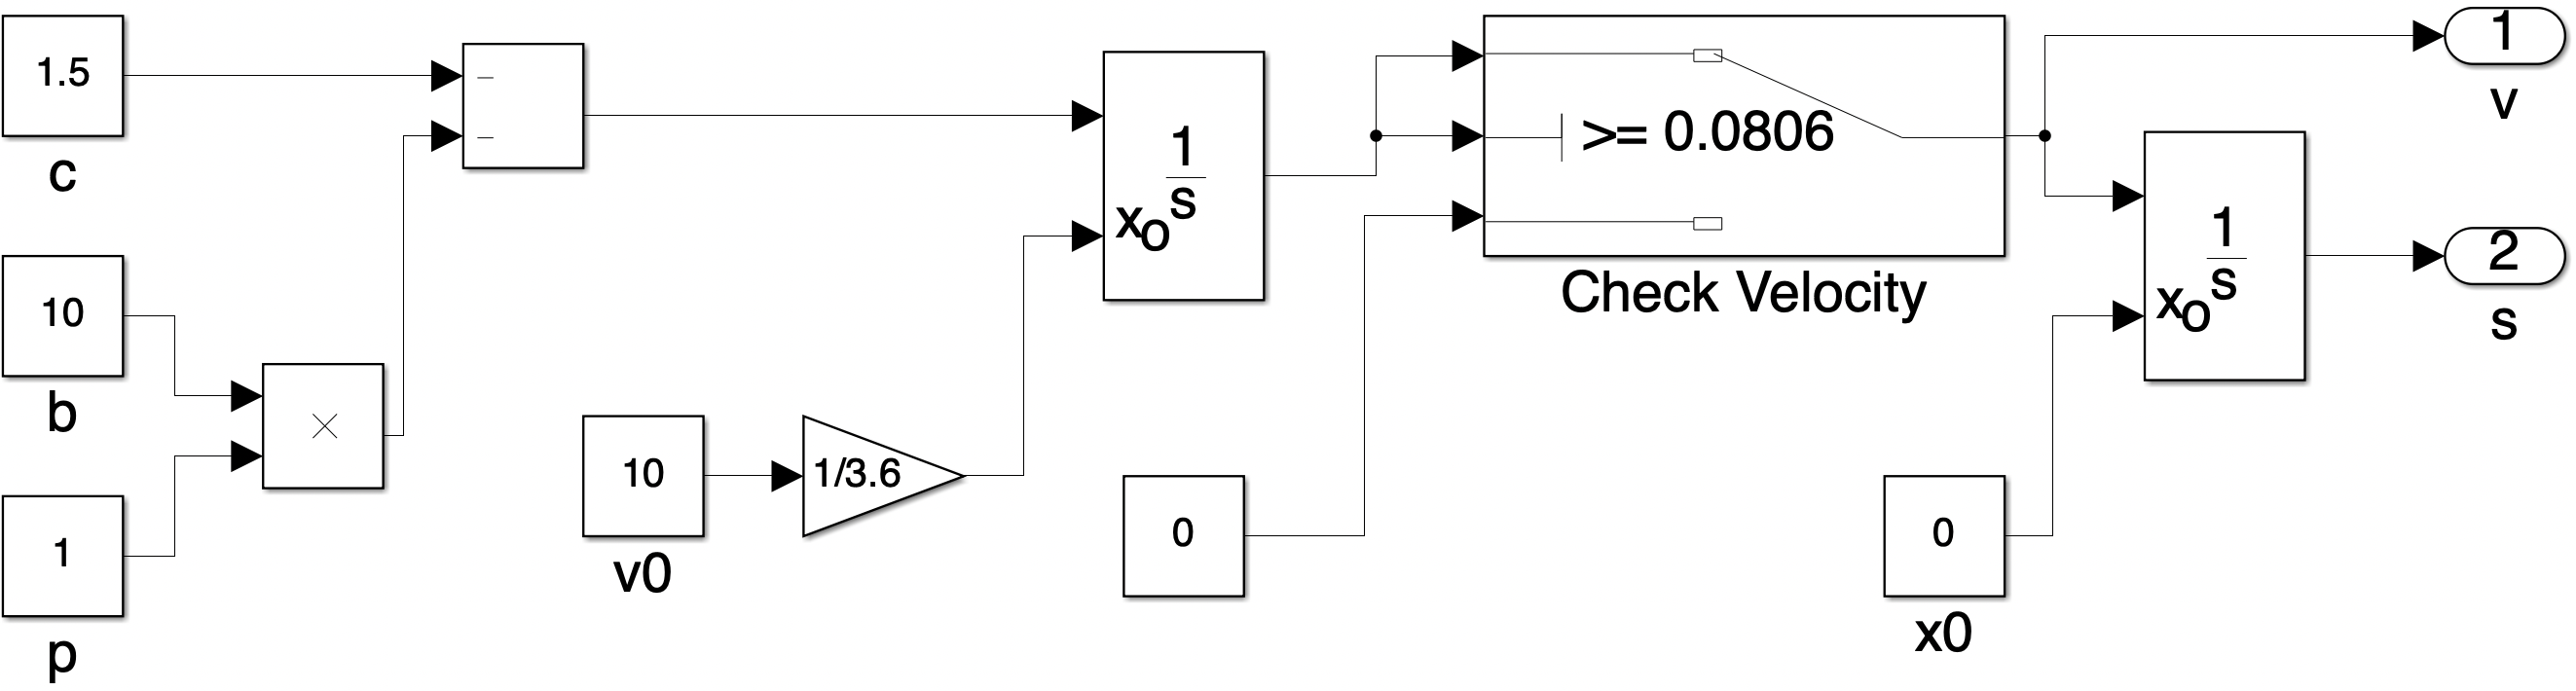
\includegraphics[width=1\textwidth]{images/D2_sim.png}
\caption{Simulink model of the differential equations}
\label{fig:D2_Sim}
\end{figure}

\section{Test scenario}\label{sec:D2_scenario}
The goal of this scenario is to check whether it is possible, with the given model, to realize a smooth stop with a stopping location < 2 m.
The idea is to demonstrate, that a full stop before 2 m can be realised with a reasonable brake pedal pressure and a reasonable deceleration.
If, for example a stop before 2 m could only be realised with 100 \% brake pressure, that would mean that a smooth stop can not be realised.\\
It is not necessary to implement a human-like smooth stop, but to show that this is possible.
Therefore the proposed test scenario is to run the model and find a reasonable small brake pressure where the car comes to a full stop with a location < 2 m.
This would show the feasibility of the task.
Creating a human-like brake profile where the brake parameter p can be adjusted over time is not an objective of this feasibility study, this will be covered at a later stage.\\
The execution of this scenario is automated using a Matlab script, which parametrizes the model and displays the outputs.
Listing \ref{lst:D2_matlab} shows the script that executes the simulation and stores the results.
The code to create the result plots has been excluded.
In lines one to eight the simulation is parametrized.
A stop time of 2 seconds is chosen because the car will come to a stop before.

todo solver begründen

The constant brake pressure is set to 5 \%.
This value results in a stop before the car traveled 2 meters of distance and is also reasonably small.

\begin{lstlisting}[language=Matlab,basicstyle=\scriptsize, caption= Execution of the feasibility test,label= lst:D2_matlab]
%% Parametrize Model
set_param('D2','StopTime','2');
%set solver
set_param('D2','Solver',['ode',sprintf('%d',8)]);
%set simulation step size
set_param('D2','FixedStep',sprintf('%f',0.01));
%set brake pressure parameter
set_param('D2/p','value',sprintf('%f',0.05));


%% Simulate and get output
res = sim('D2','SaveOutput','on','SaveState','on');
t = res.tout;
v = res.yout{1}.Values.Data;
s = res.yout{2}.Values.Data;
a = res.yout{3}.Values.Data;
%convert velocity to km/h
v = v*3.6;
\end{lstlisting}
\section{Results}\label{sec:D2_results}
The following figure \ref{fig:D2_Result} shows the simulation results with a constant brake pressure of 5\%. This results in a constant deceleration of -2 m/$s^2$. Setting the velocity to zero, when reaching the minimal velocity, has no impact on the computed acceleration. This is the reason, why the acceleration still remains the same, even though the car is not moving anymore.\\
The velocity linearly decreases from $v_0 = 10$ km/h to zero (except the decrease from minimal velocity to zero, which was expected).
The third subplot shows the covered distance of the car, which is clearly under the 2 m mark.
Therefore, with a constant brake pressure of 5 \% the car can be stopped before reaching 2 m travelled distance with an acceptable deceleration of 2 m/$s^2$. In the cruise control project we have discussed that an acceleration of less than 4 m/$s^2$ is not uncomfortable.\\
These simulation results demonstrate that it should be possible, with variation of the brake pressure over time, to realise a smooth stop with a human-like brake profile.

\begin{figure}[H]
\centering
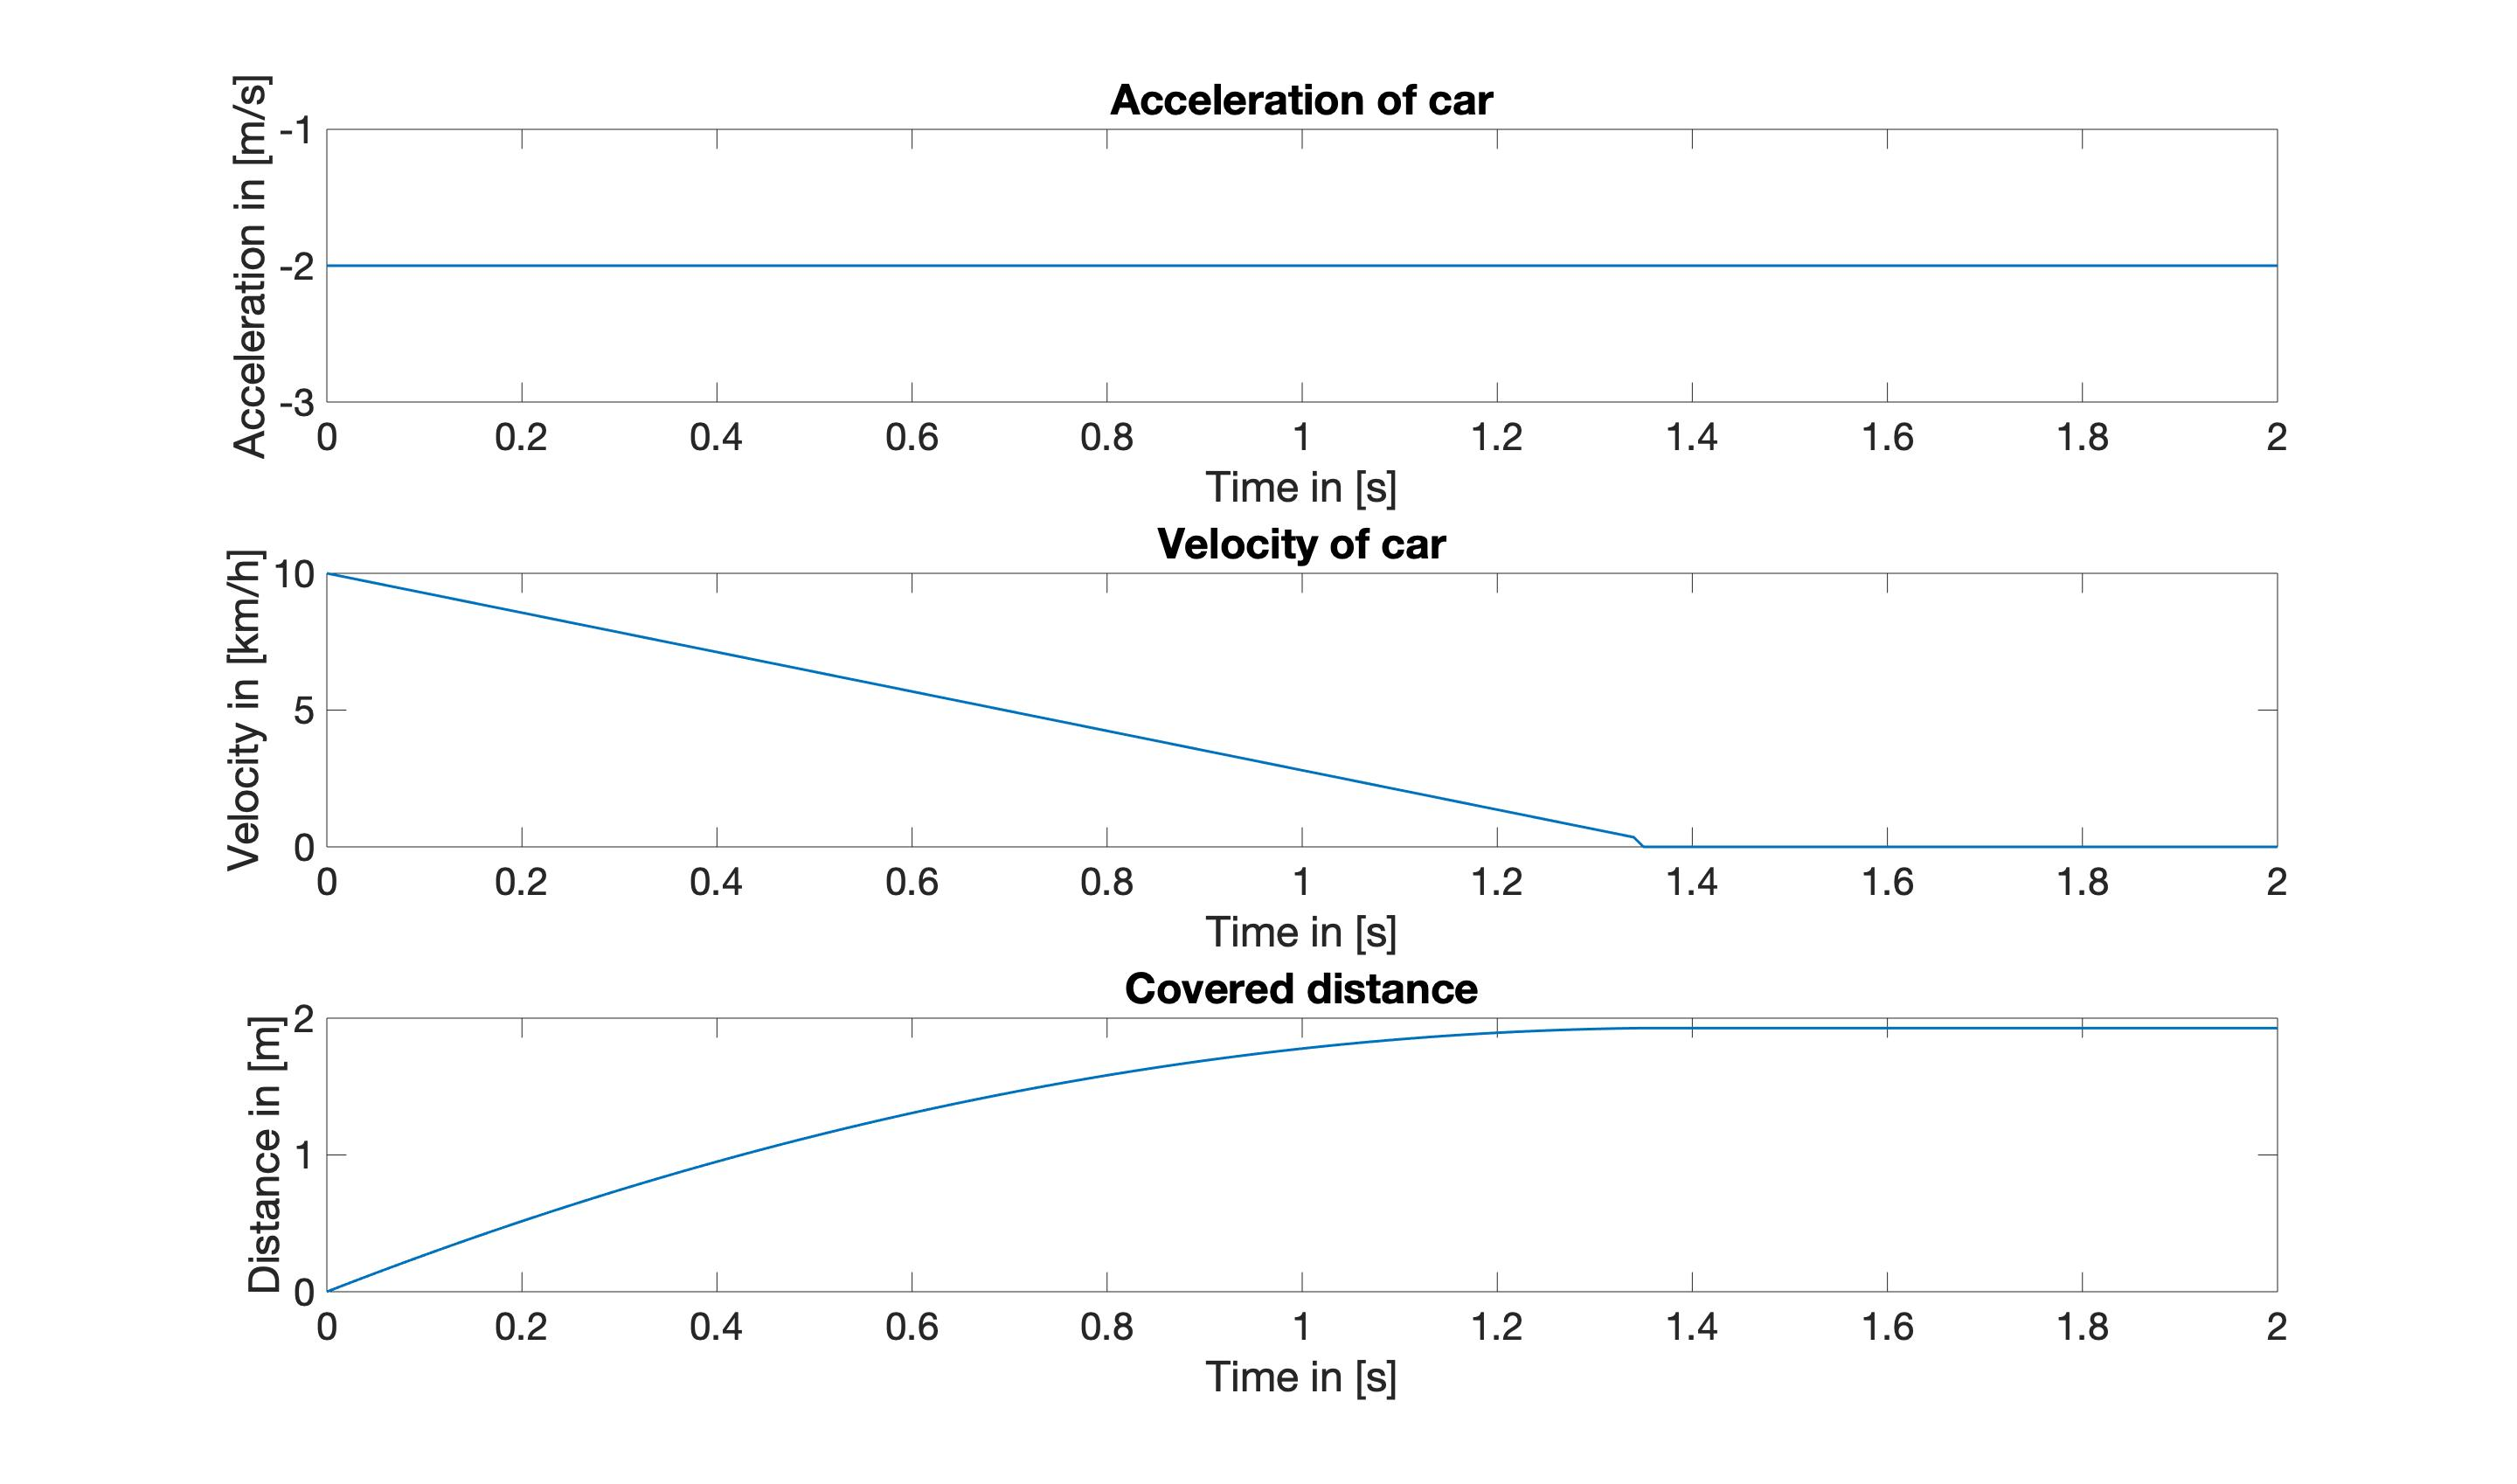
\includegraphics[width=1\textwidth]{images/D2_plot.jpg}
\caption{Simulation results of feasibility study}
\label{fig:D2_Result}
\end{figure}

\chapter{D3: Analysis of human velocity profile}\label{cha:D3}

In this section the provided human velocity profile is analysed in order to find a pattern that can be abstracted as a human-like brake profile.
This pattern will be used in the following sections and will be adapted to the braking function of the ParkAssist.
For the analysis Matlab functions are used, as demanded by requirement D3.
\section{Import the measurement data}
The human velocity profile contains a time dimension and the four wheel velocities.
The following listing shows how the measurement data is imported in Matlab.
A Matlab library function is used for the import of the textfile.
This results in a standard numeric matrix.

\begin{lstlisting}[language=Matlab,basicstyle=\scriptsize	,caption= Import measurement data in Matlab,label= lst:D3Import]
%import velocity data
velocity_data = importdata('MeasuredVelocities.txt');
\end{lstlisting}

\section{Data preparation}
The aim of the analysis is to make conclusions that lead to a time dependant brake profile.
Since the brake pedal has a linear influence on the acceleration (see model formula) the goal is to extract an acceleration curve from the human velocity profile, from which to make deductions on the brake profile.
For that, a cars acceleration and in consequence the cars velocity is needed.
Therefore a mean car velocity has to be extracted from the given four wheel velocities.

Listing \ref{lst:D3Preprocess} shows the Matlab script that pre-processes the data.
As a first step, the four wheel velocities are extracted from the measurement data and a mean velocity is calculated with the following equation (lines 2 and 3 in listing \ref{lst:D3Preprocess}):
\begin{equation}
	v_{car} = (v_{w1} +v_{w2} + v_{w3} +v_{w4})/4
\end{equation}
This mean velocity serves as an estimate for the car velocity.
It is only an estimate, because friction losses, other physical influences and cornering are not considered.
The mean velocity is converted to [m/s] for further calculations in line 4 in listing \ref{lst:D3Preprocess}.
Before calculating the acceleration, a moving average filter is applied on the mean velocity (line 8 in listing \ref{lst:D3Preprocess}). Further details about the moving average filter are given in the next paragraph.
The acceleration can be calculated by differentiating the mean velocity (line 11 in listing \ref{lst:D3Preprocess}).

\begin{lstlisting}[language=Matlab,basicstyle=\scriptsize	,caption= Preprocessing measurement data,label= lst:D3Preprocess]
%compute mean velocity of all 4 wheels
velocity_per_wheel = velocity_data(:,2:5);
mean_velocity = mean(velocity_per_wheel,2);
mean_velocity = mean_velocity/3.6;      %convert velocity from km/h to m/s
raw_mean_velocity = mean_velocity;      %for demonstration purposes

%apply moving average filter to smoothen the data
mean_velocity = movmean(mean_velocity, 200); 

%differentiate velocity to get acceleration
acceleration = diff(mean_velocity);
raw_acceleration = diff(raw_mean_velocity);     %for demonstration purposes
\end{lstlisting}

As can be seen in the upper subplot of figure \ref{fig:D3_MovingAverage} the calculated acceleration is noisy due to noise in the measured velocity.
Because of the noise it would be harder to analyse the braking behaviour. Therefore we used a moving average filter to smoothen the data.
A moving average filter is calculating a mean value of neighbouring elements within a sliding window of a predefined size.
Applying a moving average filter results in a filtered graph that can bee seen in the lower subplot of figure \ref{fig:D3_MovingAverage}. 
However, applying a moving average filter distorts the acceleration values because the exact value is replaced by the average of the neighbouring elements. This reduces the difference between the values of neighbouring elements.
As a result the differentiation of the velocity results in an acceleration that is in our case approximately 10 times smaller than the non-filtered results.
Although the values of the acceleration are smaller the course of the acceleration is not changed.
Therefore the filtered data is not used to extract exact acceleration values but rather to get an understanding of the acceleration curve during braking.\\

%Figure \ref{fig:D3_MovingAverage} shows the impact of the moving average filter on the car velocity.
%The course of the graph still the same, even though the absolute values are smaller that the unfiltered acceleration because of the before mentioned reasons.
\begin{figure}[H]
\centering
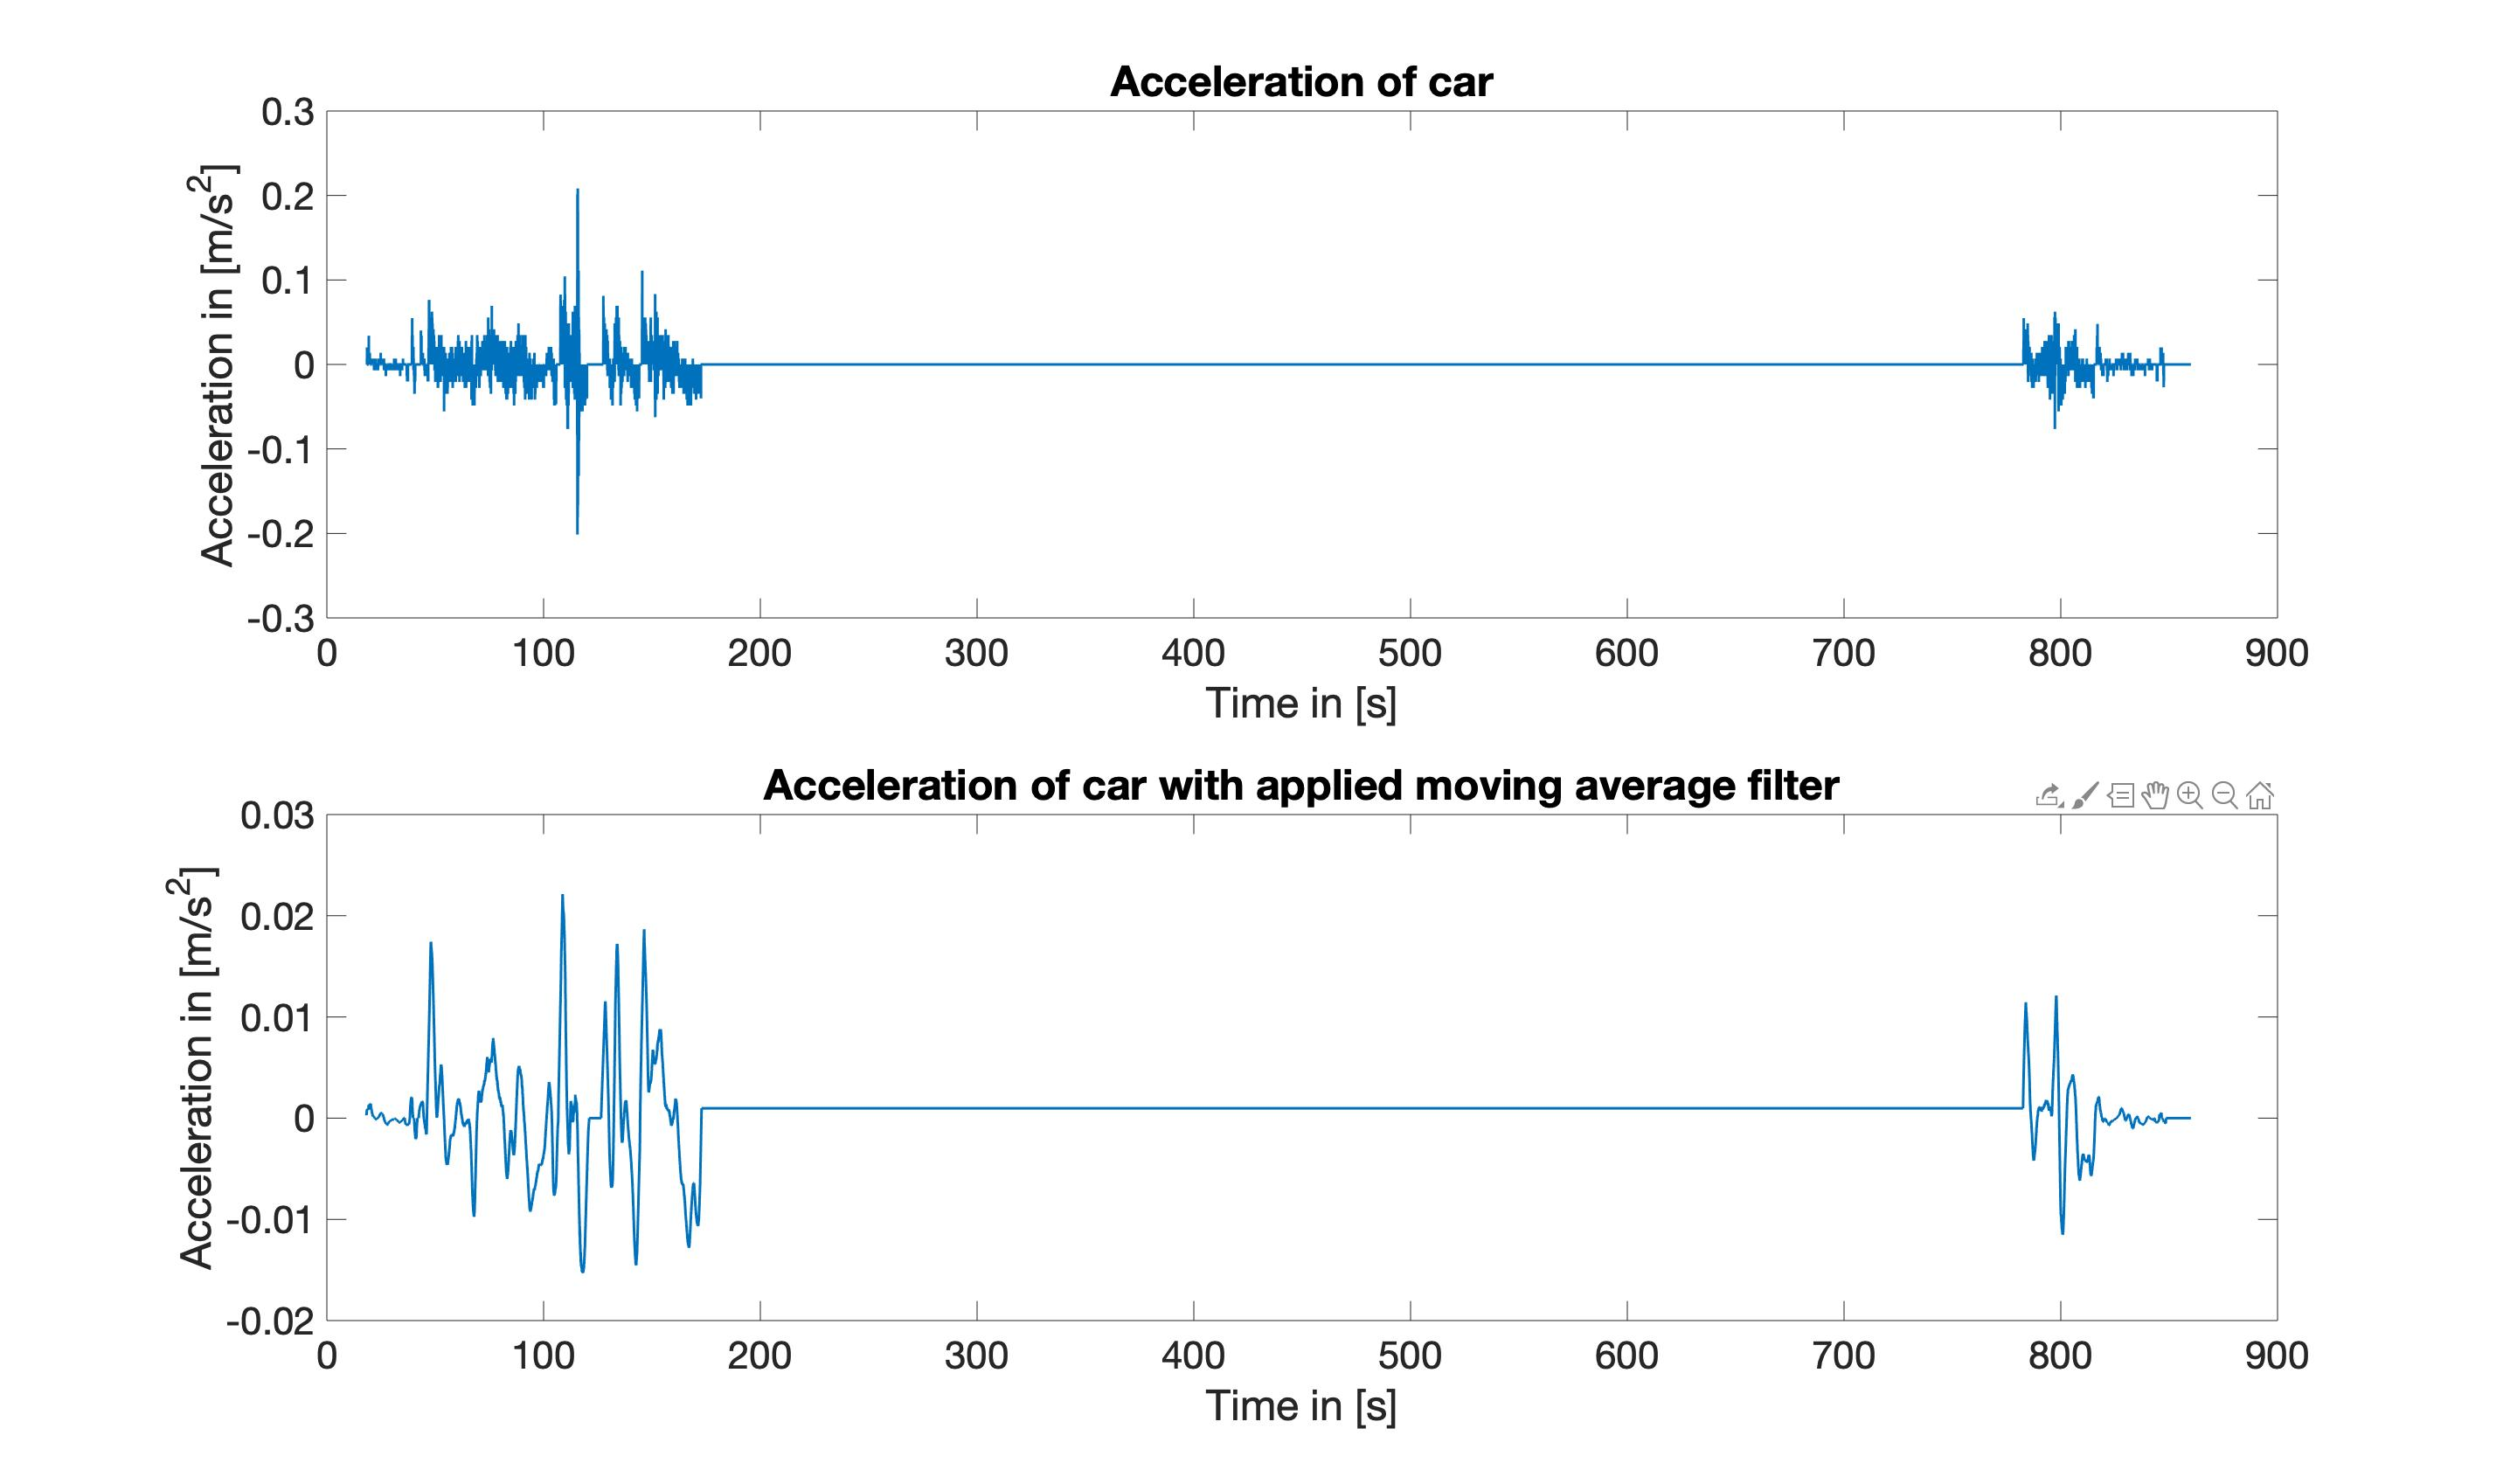
\includegraphics[width=1\textwidth]{images/D3_moving_average.jpg}
\caption{Impact of applying a moving average filter on the cars acceleration}
\label{fig:D3_MovingAverage}
\end{figure}

Figure \ref{fig:D3_Fig_Overview} shows the mean velocity of the car as well as the corresponding smoothened acceleration of the car over time.

\begin{figure}[H]
\centering
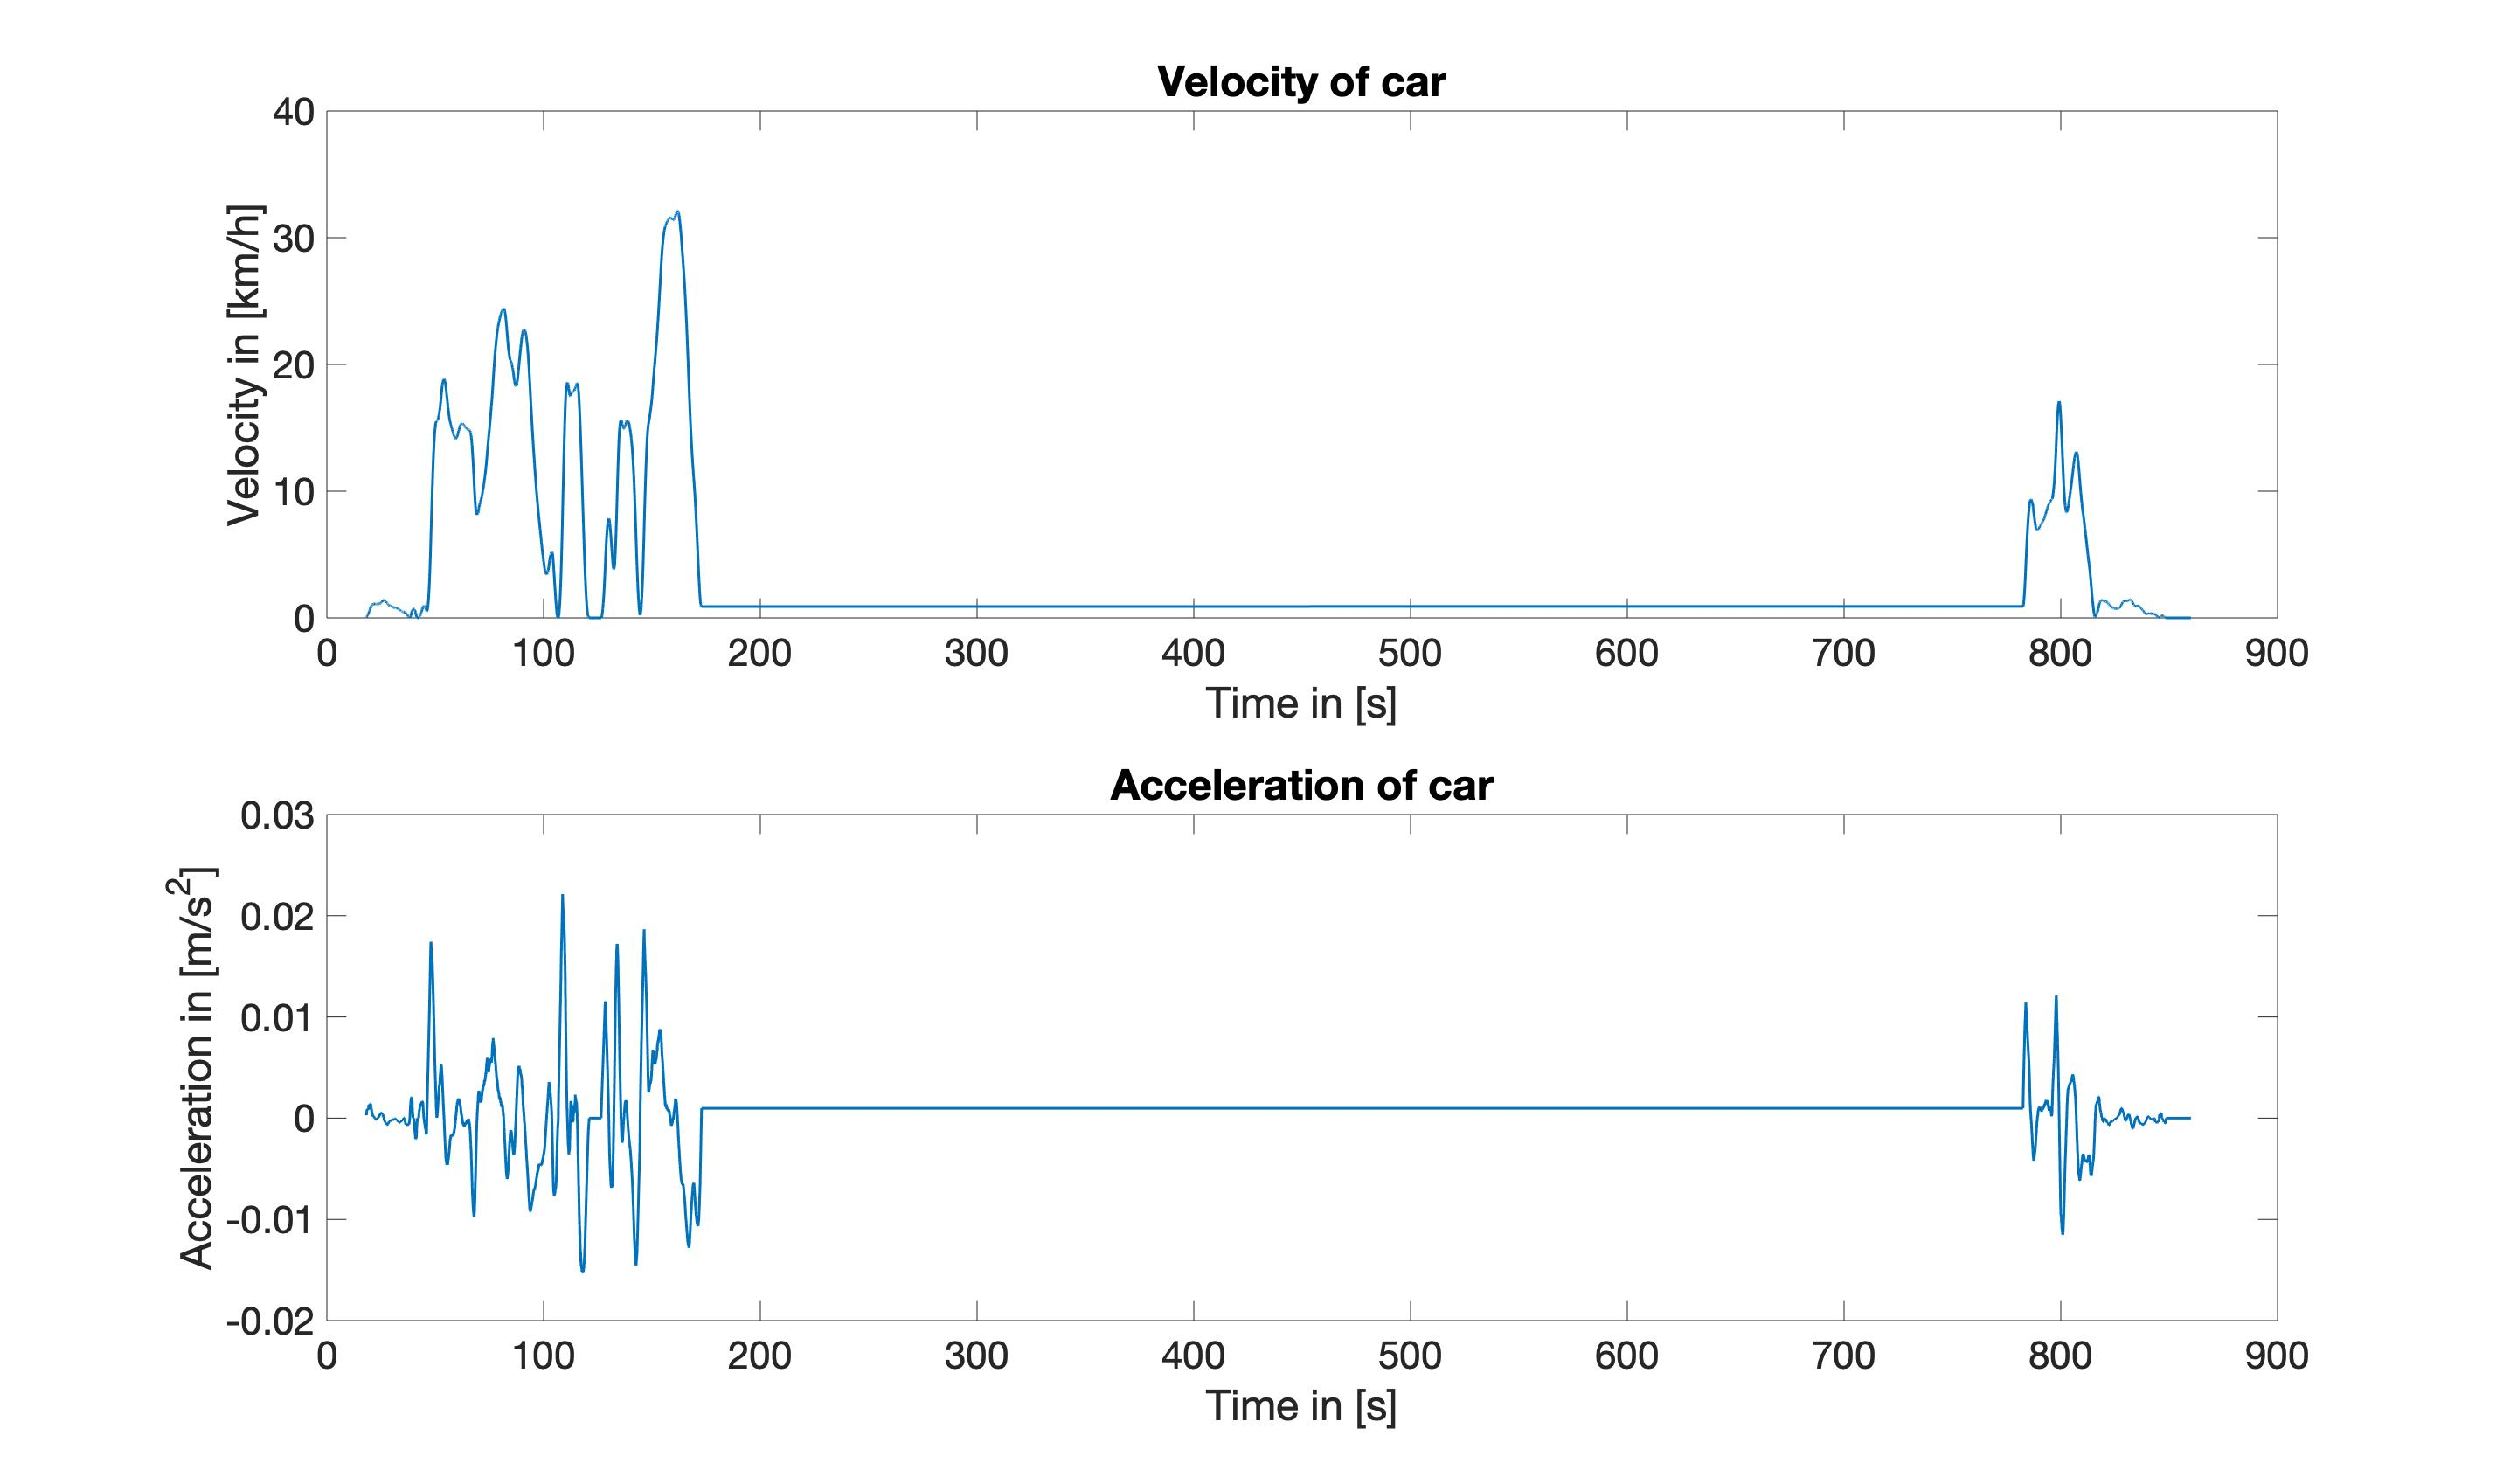
\includegraphics[width=1\textwidth]{images/D3_Fig_Overview.jpg}
\caption{Extracted human velocity profile}
\label{fig:D3_Fig_Overview}
\end{figure}


\section{Extracting negative acceleration}
As the goal is to analyse the braking behaviour, only negative acceleration is relevant and is thus being extracted from the overall acceleration (line 5 in listing \ref{lst:D3Extract}). Also, all velocities that are based on a positive acceleration are not considered anymore (line 6 in listing \ref{lst:D3Extract}). We decided to set those values to \ac{NaN} because this way we are still able to plot the velocity and the acceleration over time without cut-outs. The result can be seen in figure \ref{fig:D3_IndividualBraking}. 

\begin{lstlisting}[language=Matlab,basicstyle=\scriptsize	,caption= Extracting negative acceleration,label= lst:D3Extract]
%search for negative acceleration and set positive acceleration to NaN
%set all velocities that have a positive acceleration to NaN
neg_acceleration = acceleration;
decreasing_velocity = mean_velocity;
neg_acceleration(neg_acceleration>0) = nan;
decreasing_velocity(isnan(neg_acceleration)) = nan;
\end{lstlisting}

\begin{figure}[H]
\centering
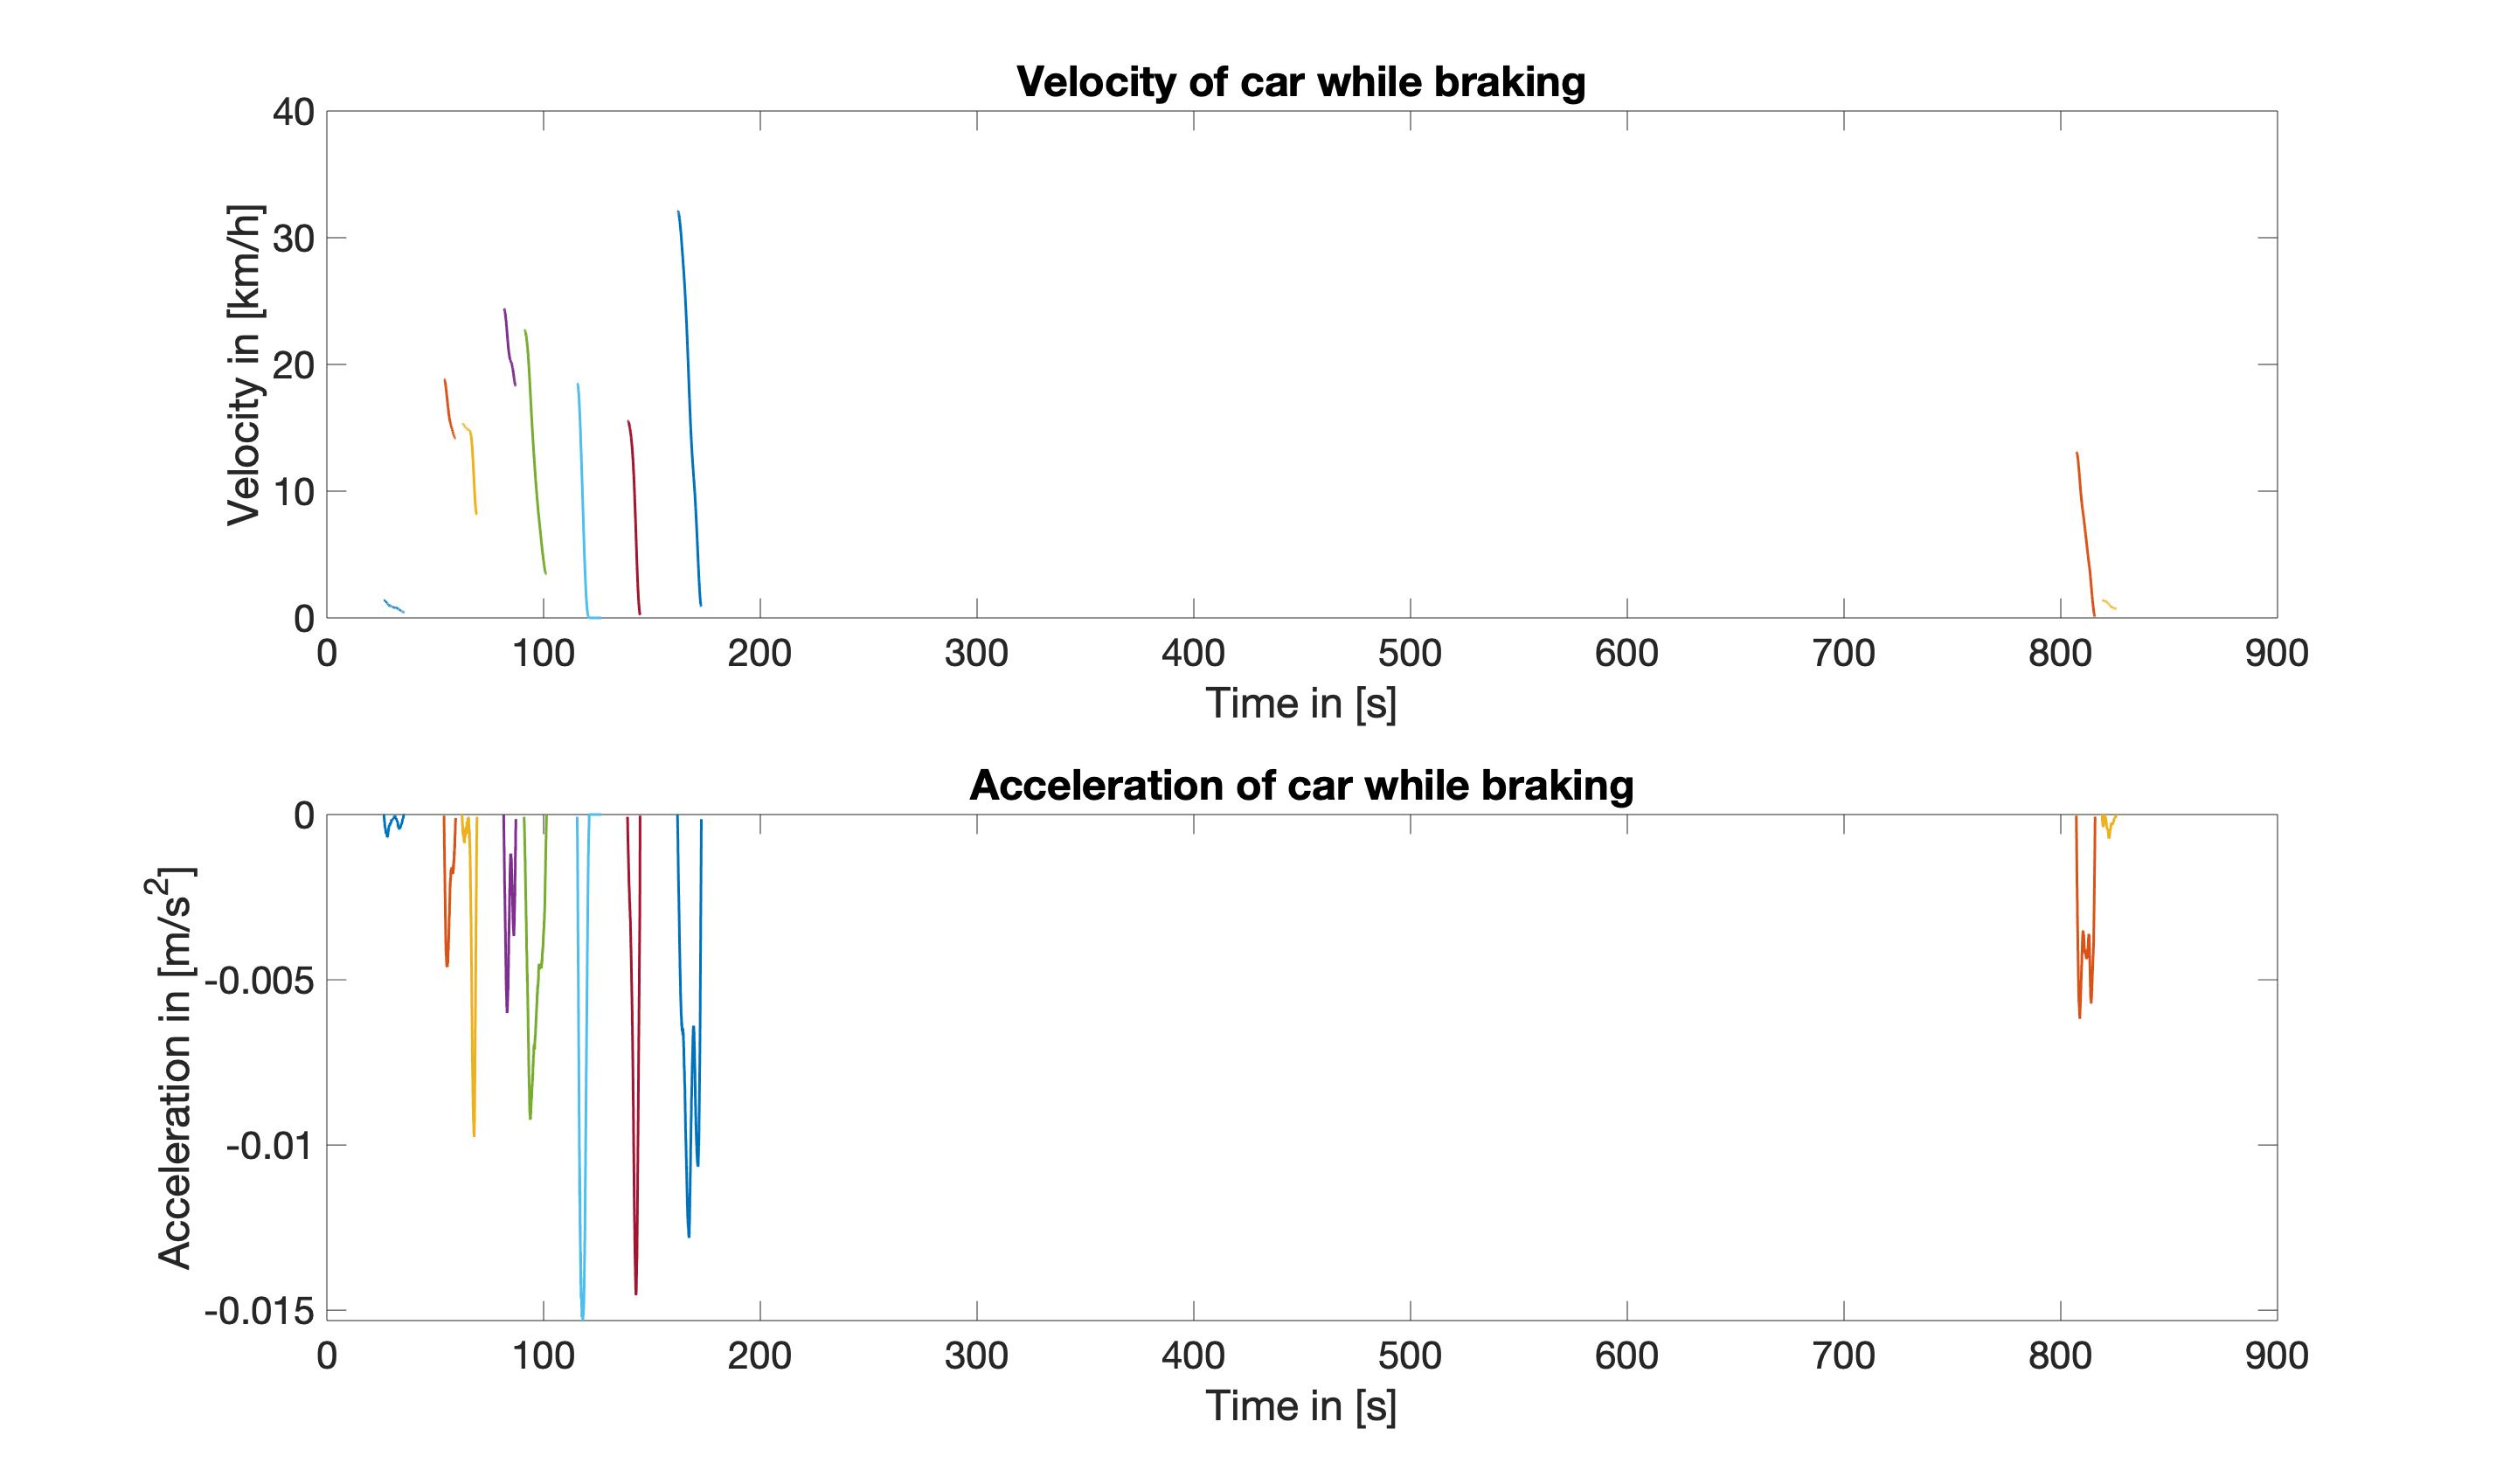
\includegraphics[width=1\textwidth]{images/D3_individual_braking.jpg}
\caption{Braking manoeuvres in human velocity profile}
\label{fig:D3_IndividualBraking}
\end{figure}


\section{Separating breaking sequences}
For better visualisation, the breaking sequences that can be seen in figure \ref{fig:D3_IndividualBraking} will be stored separately.
One breaking sequence consists of multiple consequent velocity measurements.
This means that the breaking sequences can be separated by searching for a gap in the velocity measurements (\ac{NaN} values).
Therefore, the indices of all velocities that are set not \ac{NaN} are extracted (line 2 in listing \ref{lst:D3Seperat}) and differentiated (line 3 in listing \ref{lst:D3Seperat}).
Consequently, every differentiation that is greater than 1 marks a gap between velocities because indices of one braking sequence are subsequent (differentiation equals 1).
Furthermore, short breaking sequences are not considered because they are most likely not relevant for recognizing a breaking pattern (line 13 in listing \ref{lst:D3Seperat}).
Two individual breaking sequences can be seen in figure \ref{fig:D3_IndividualBraking1} and figure \ref{fig:D3_IndividualBraking2}.

\begin{lstlisting}[language=Matlab,basicstyle=\scriptsize	,caption= Separating breaking sequences,label= lst:D3Seperat]
%find individual breaking sequences
notNaN_velocity = find(~isnan(decreasing_velocity));   % find index of every velocity that is not NaN -> one breaking sequence has consequent time steps -> one breaking sequence has consequent indices
diff_notNaN_velocity = diff(notNaN_velocity);          % differentiate indices -> if indices are not consequent (unequal 1), a new breaking sequence has begun
n = 1;                                                 % set start values
start = 1;

%seperate breaking sequences with previous findings
for i=1:length(diff_notNaN_velocity)
    %for every index check if indices are consequent -> equals 1
    if diff_notNaN_velocity(i) > 1
        %if not check if a breaking sequence consists of min 500 time
        %steps, this way small breaking sequences are sorted out
        if (i-start) > 500
            %add breaking sequence to section
            %i is end of sequence
            section{n} = notNaN_velocity(start:i);
            %start for new sequence is end of old sequence + 1
            start = i+1;
            %increment n
            n = n+1;
        else
            %if breaking sequence is to small, set start for new sequence
            %to end of old sequence + 1 anyway
            start = i+1;
        end
    end
end
\end{lstlisting}


\begin{figure}[H]
\centering
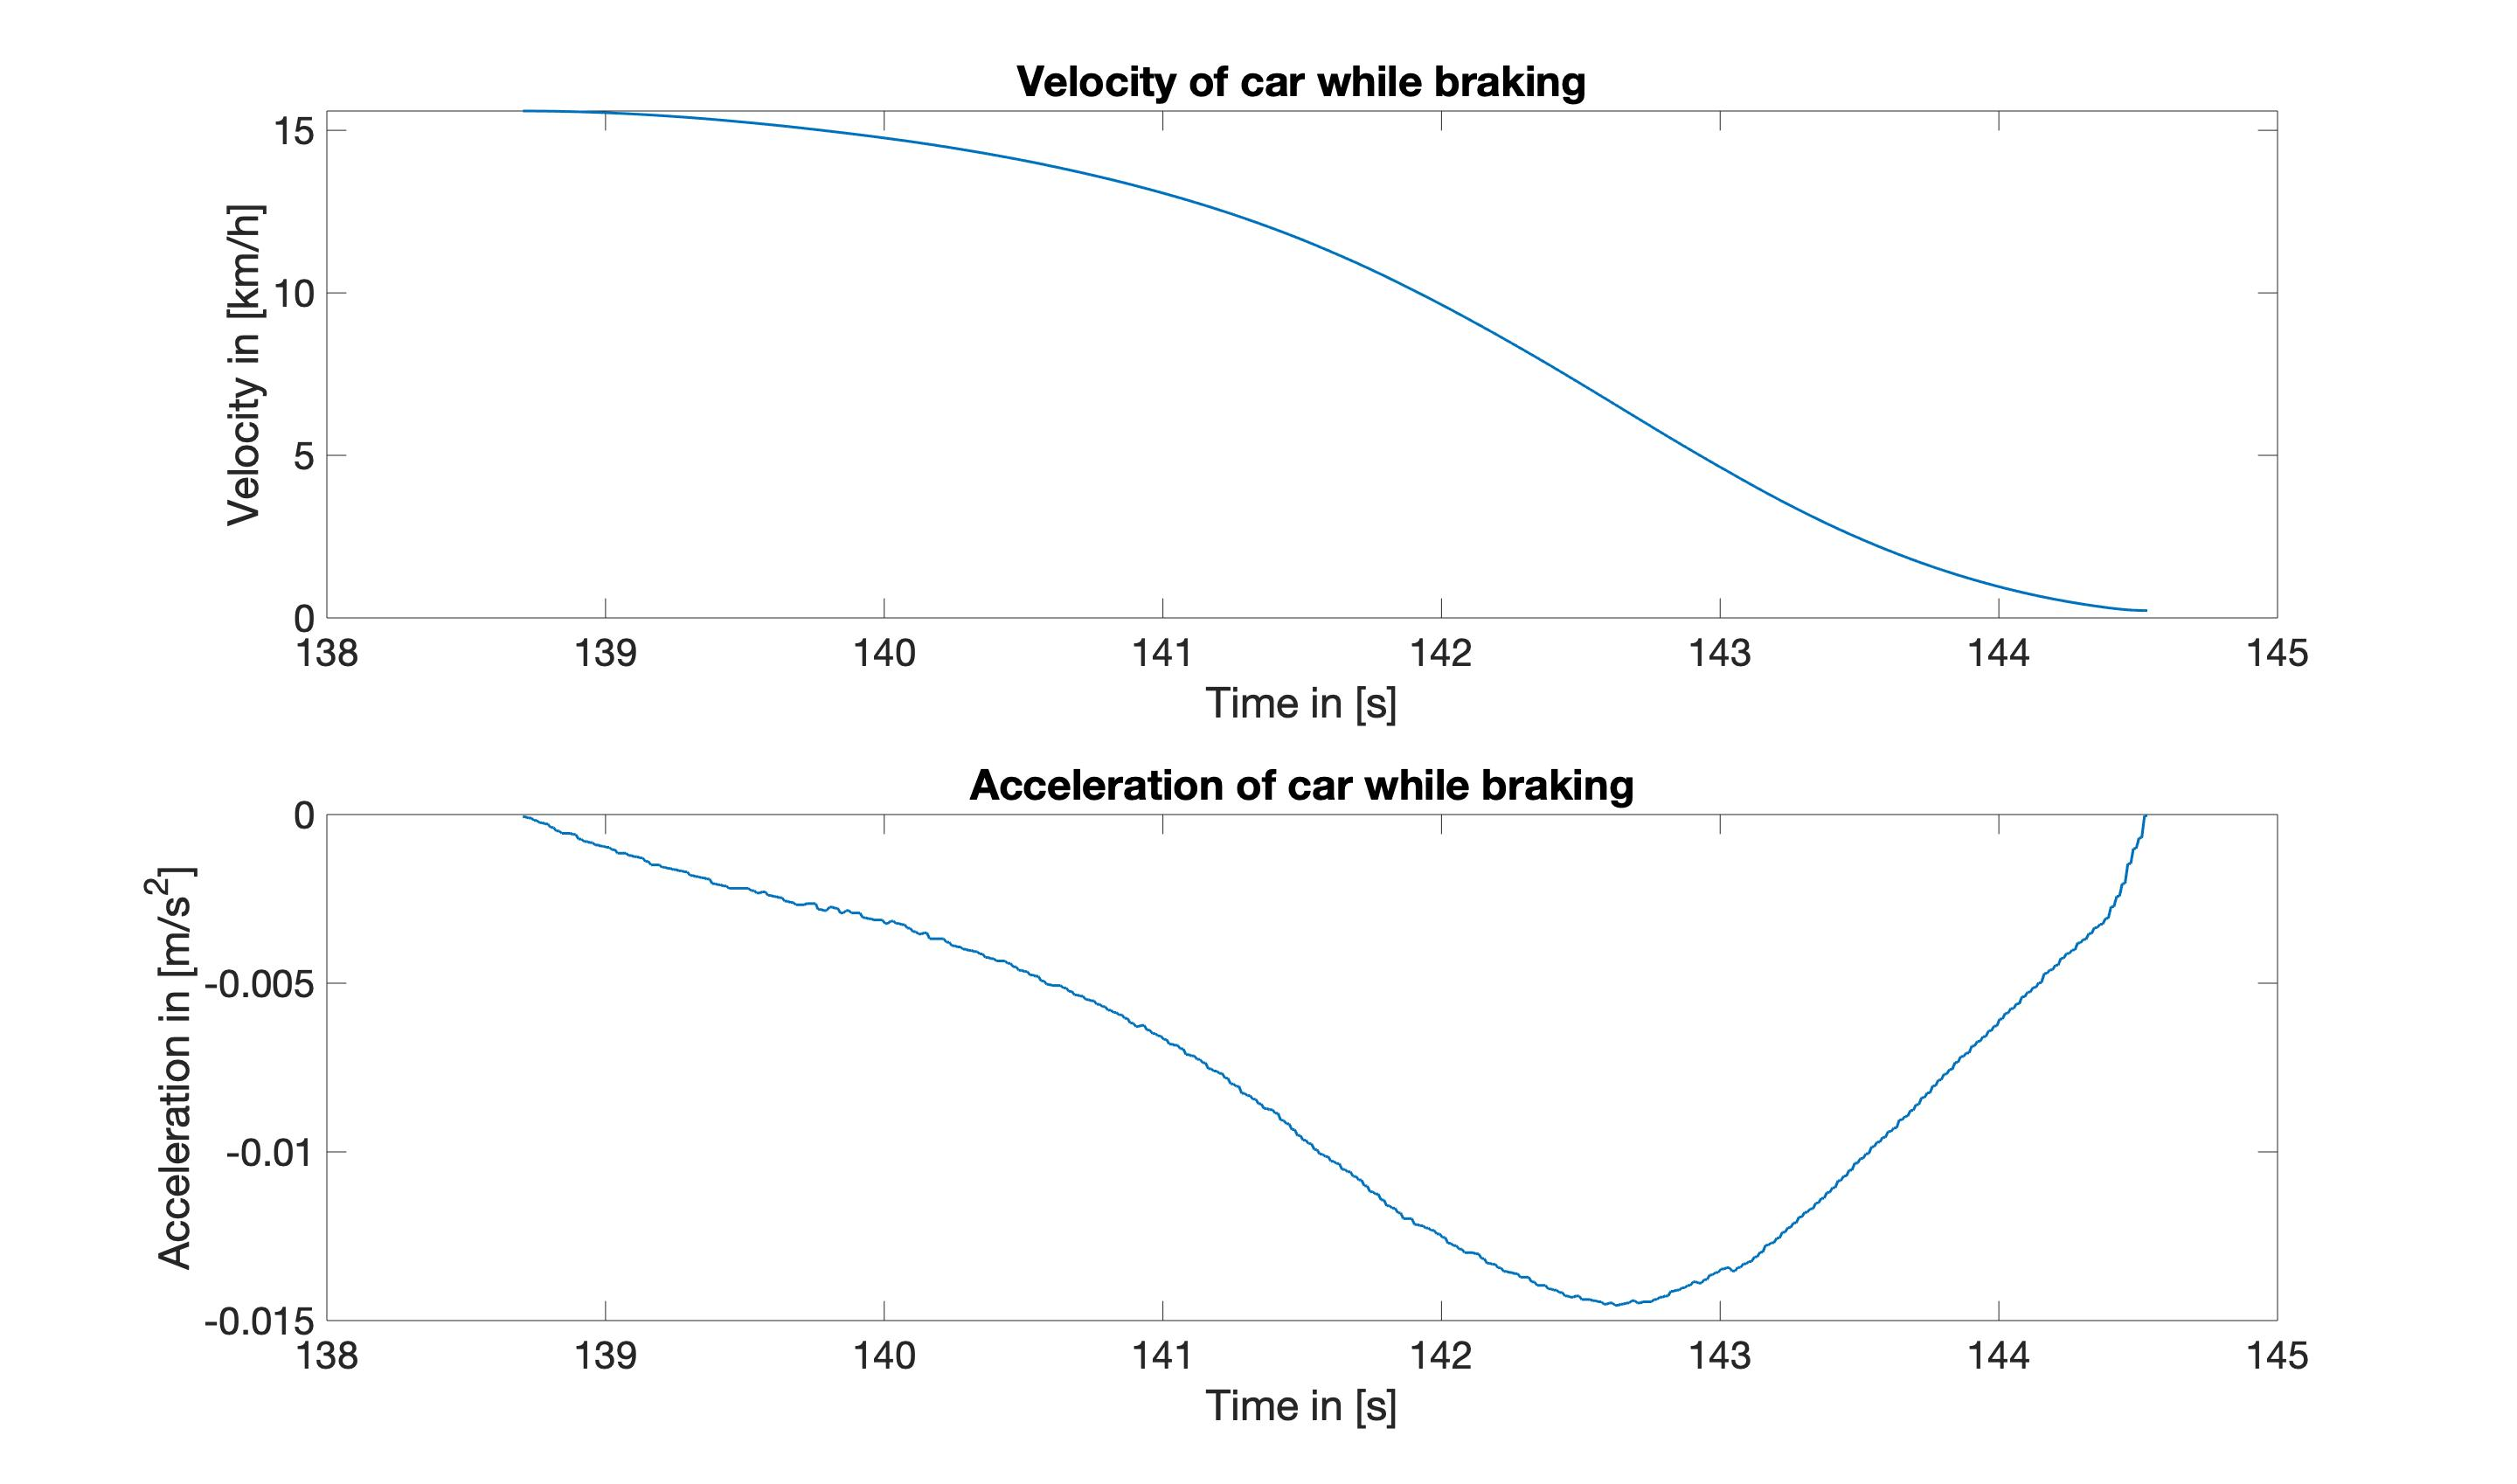
\includegraphics[width=1\textwidth]{images/D3_example1.jpg}
\caption{Individual braking manoeuvre 1 extracted from the human velocity profile}
\label{fig:D3_IndividualBraking1}
\end{figure}

\begin{figure}[H]
\centering
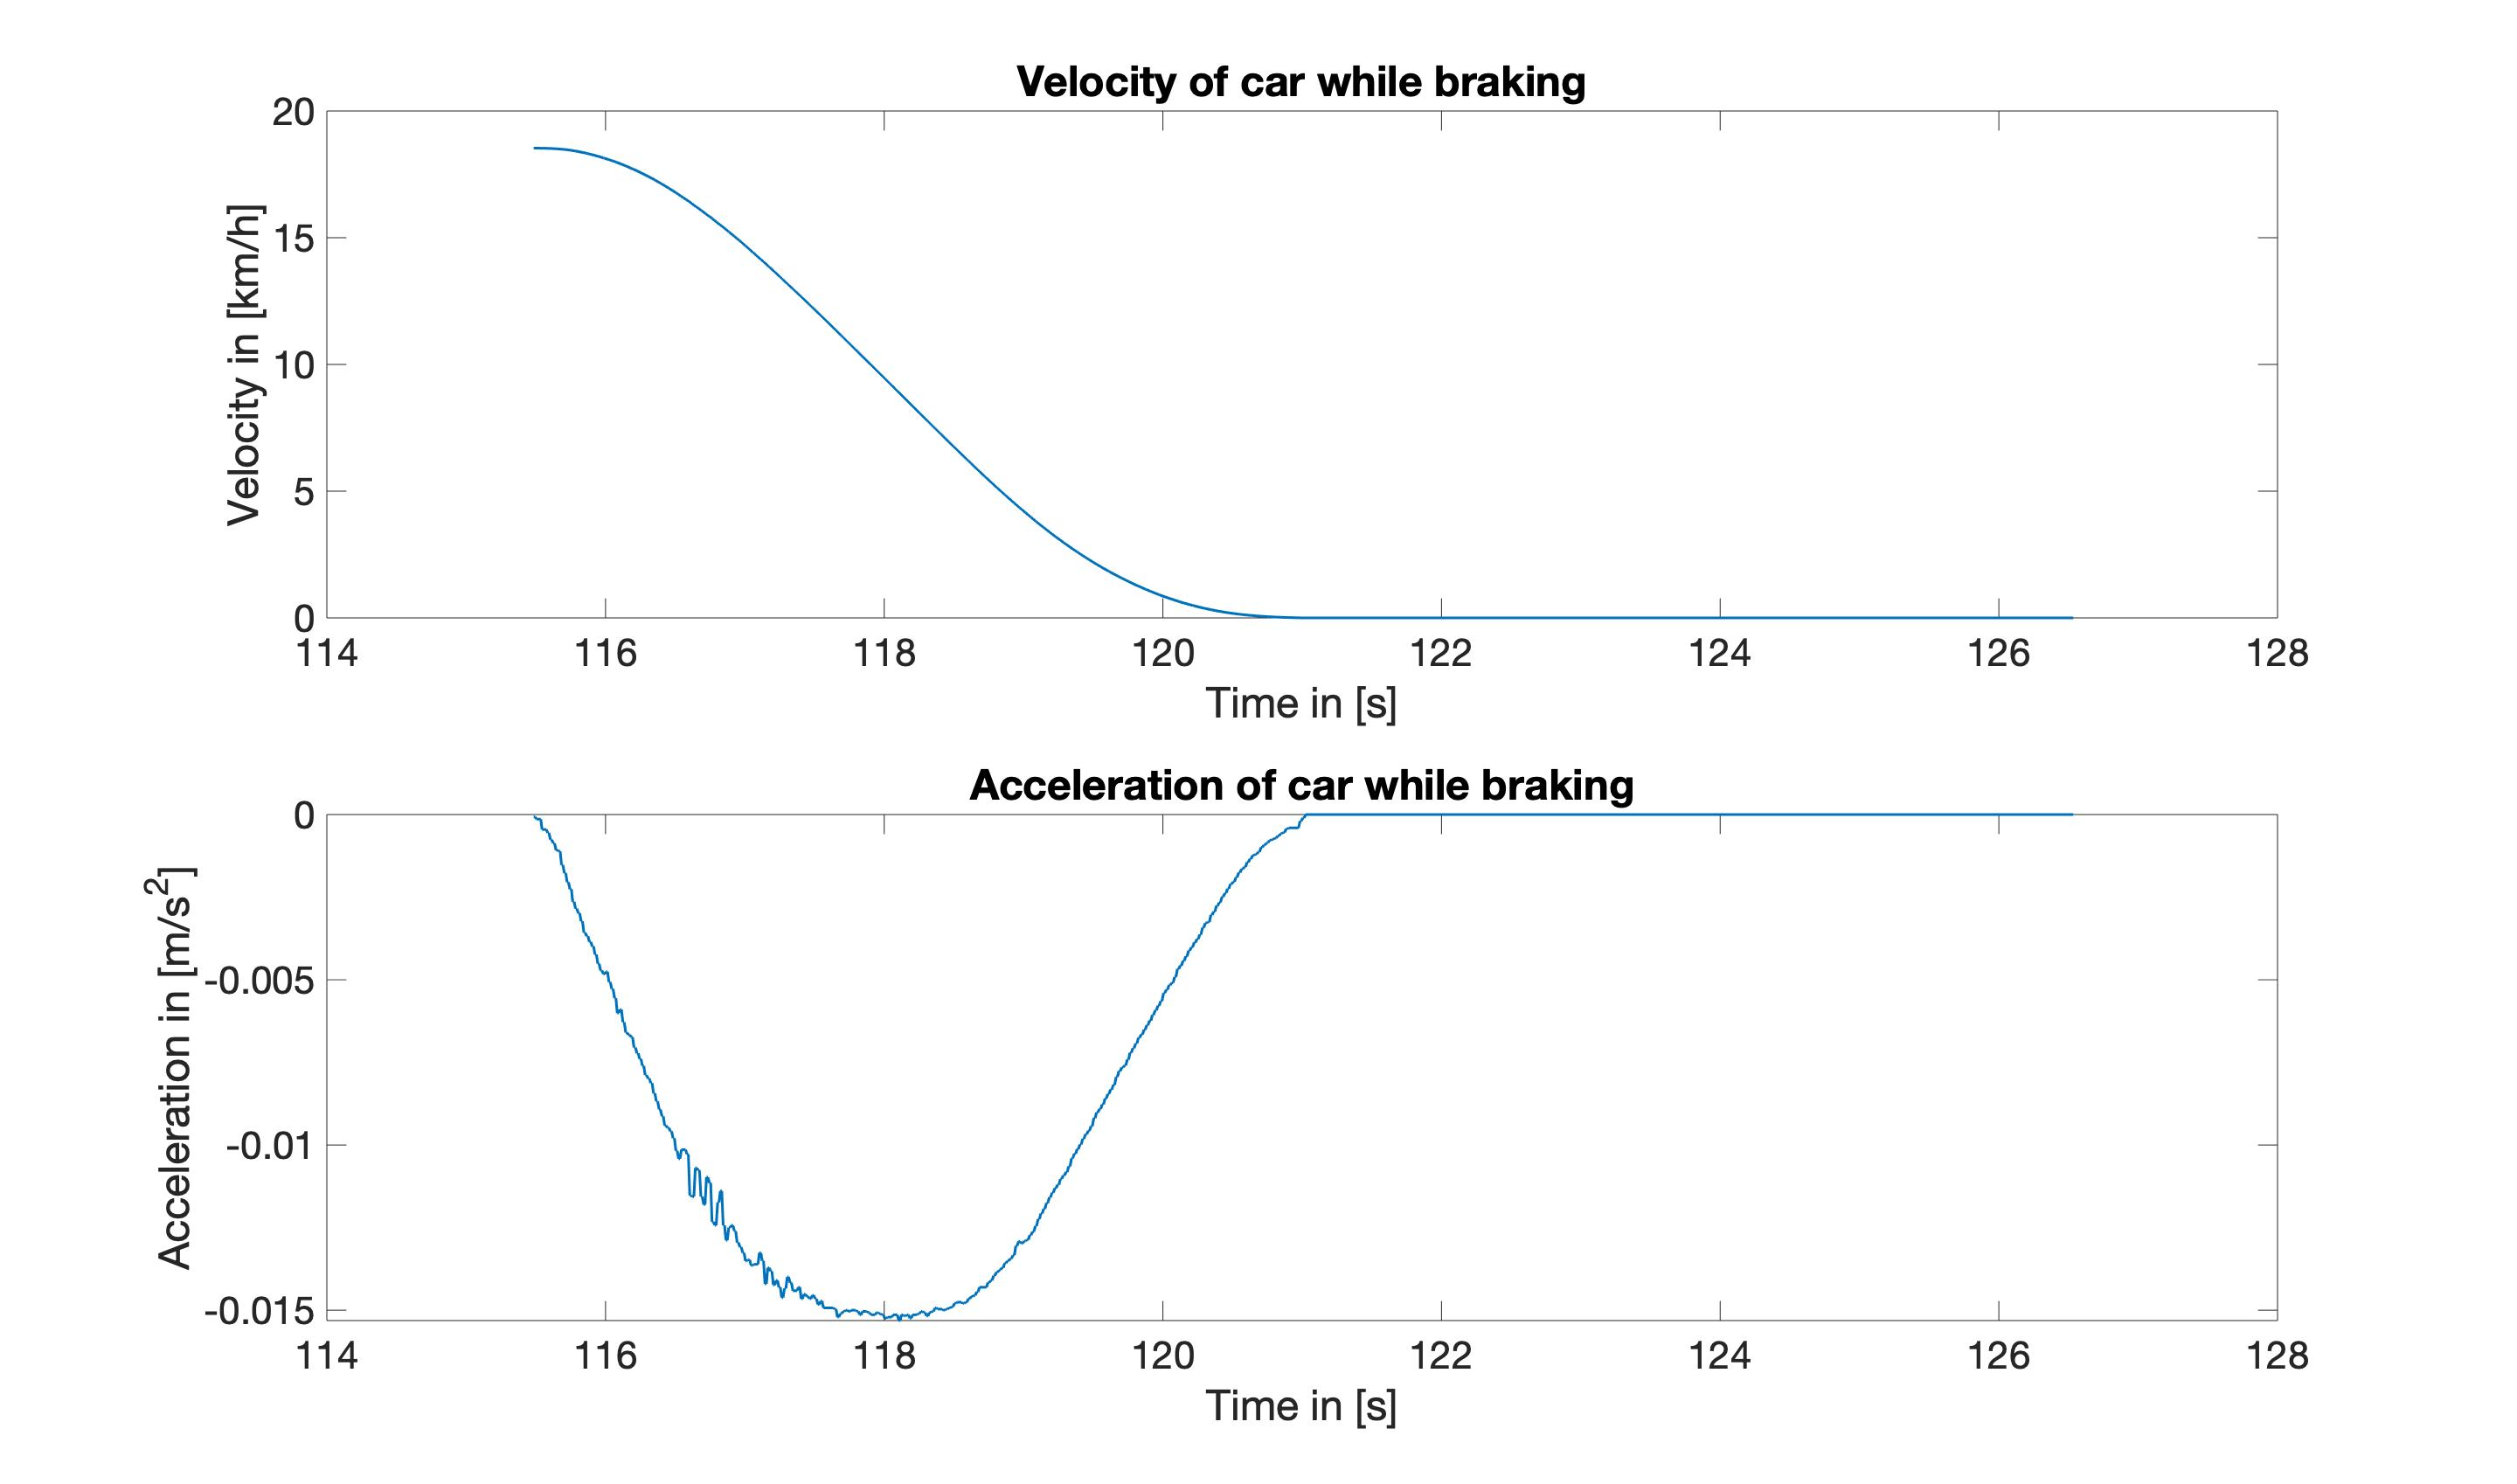
\includegraphics[width=1\textwidth]{images/D3_example2.jpg}
\caption{Individual braking manoeuvre 2 extracted from the human velocity profile}
\label{fig:D3_IndividualBraking2}
\end{figure}

\section{Results}
Considering figures \ref{fig:D3_IndividualBraking1} and \ref{fig:D3_IndividualBraking2}, it can be seen that the acceleration is approximately in the shape of a downward facing parable. This results in the velocity decreasing slowly in the beginning, then decreasing more severly and flattening in the end.   
%For further implementation of the ParkAssist, we will start the breaking process with an acceleration and increase it until we reach approximately REF and will then decrease it.

%entschieden Durchschnitt der vier Radgeschwindigkeiten zu nehmen (vllt. vor nachteile)
%und so auf die Geschwindigkeit des Autos näherungsweise zu bestimmen
%
%todo hier plot von gesamtgeschwindigkeit
%
%idee: verzögerungsphasen extrahieren um so auf "menschliche" negative beschleunigung zu schließen
%problem: verrauschte messdaten -> dadurch ständiger wehcsel positive negative beschleunigung
%
%lösung: moving average filter zum glätten der messwerte
%dann extrahieren der negativen beschleunigungen

\section{Development of p(t)}\label{sec:D3_dev_pt}
%with no brake:
%-model from D2
%-stopped after 1.8s, at approx 2.6m
%\begin{figure}[H]
%\centering
%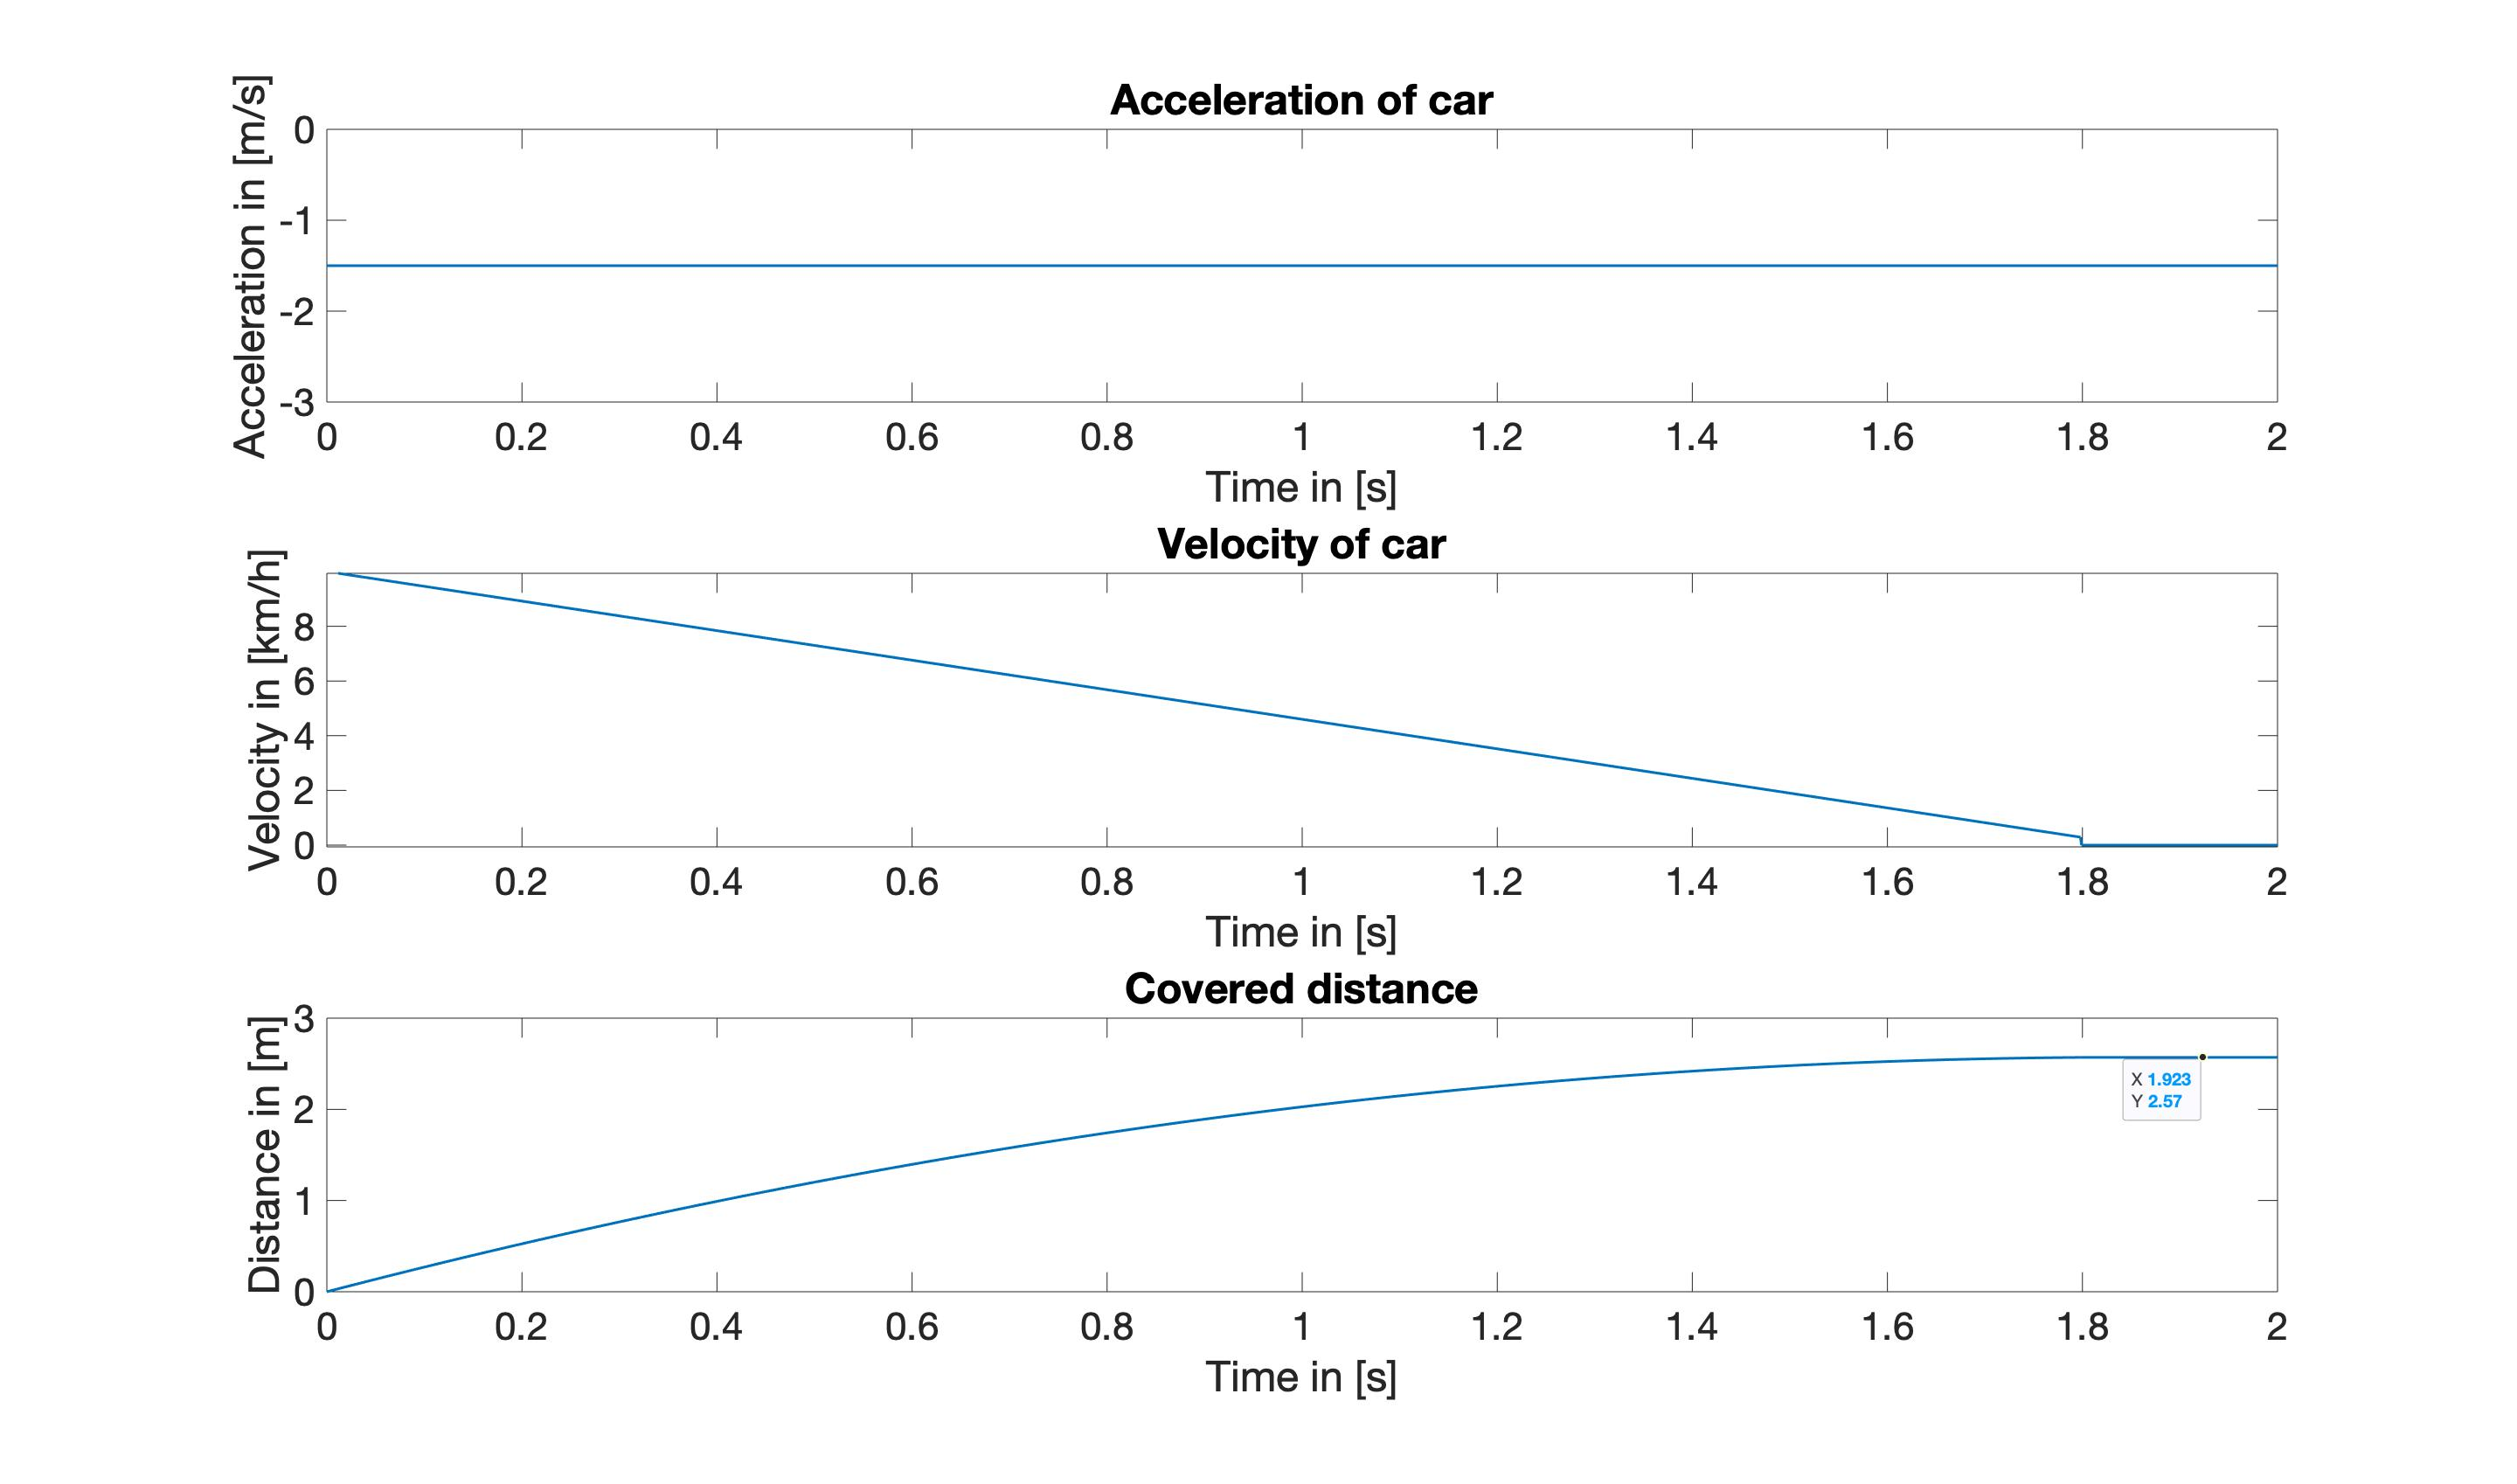
\includegraphics[width=1\textwidth]{images/D3_no_brake.jpg}
%\caption{Simulation without braking}
%\label{fig:D3_IndividualBraking2}
%\end{figure}

The goal is to find a p(t) with an acceleration curve similar to the extracted above.
Since the brake pedal position has a linear negative influence on the acceleration, the brake pedal function should press the brake pedal with an approximate parabola that is opened downwards.
This ensures a smooth braking behaviour with slowly starting braking and also easing of the brake at the end of the manoeuvre, using friction to come to a full stop (like the driving teacher suggested).

To simulate a time dependant brake pressure the before developed Simulink model (see section \ref{sec:D2_model}) has been extended with a lookup-table that contains the brake pressure parameters.
The integrator that integrates the constant 1 provides the time input to the lookup table (lower left corner).
\begin{figure}[H]
\centering
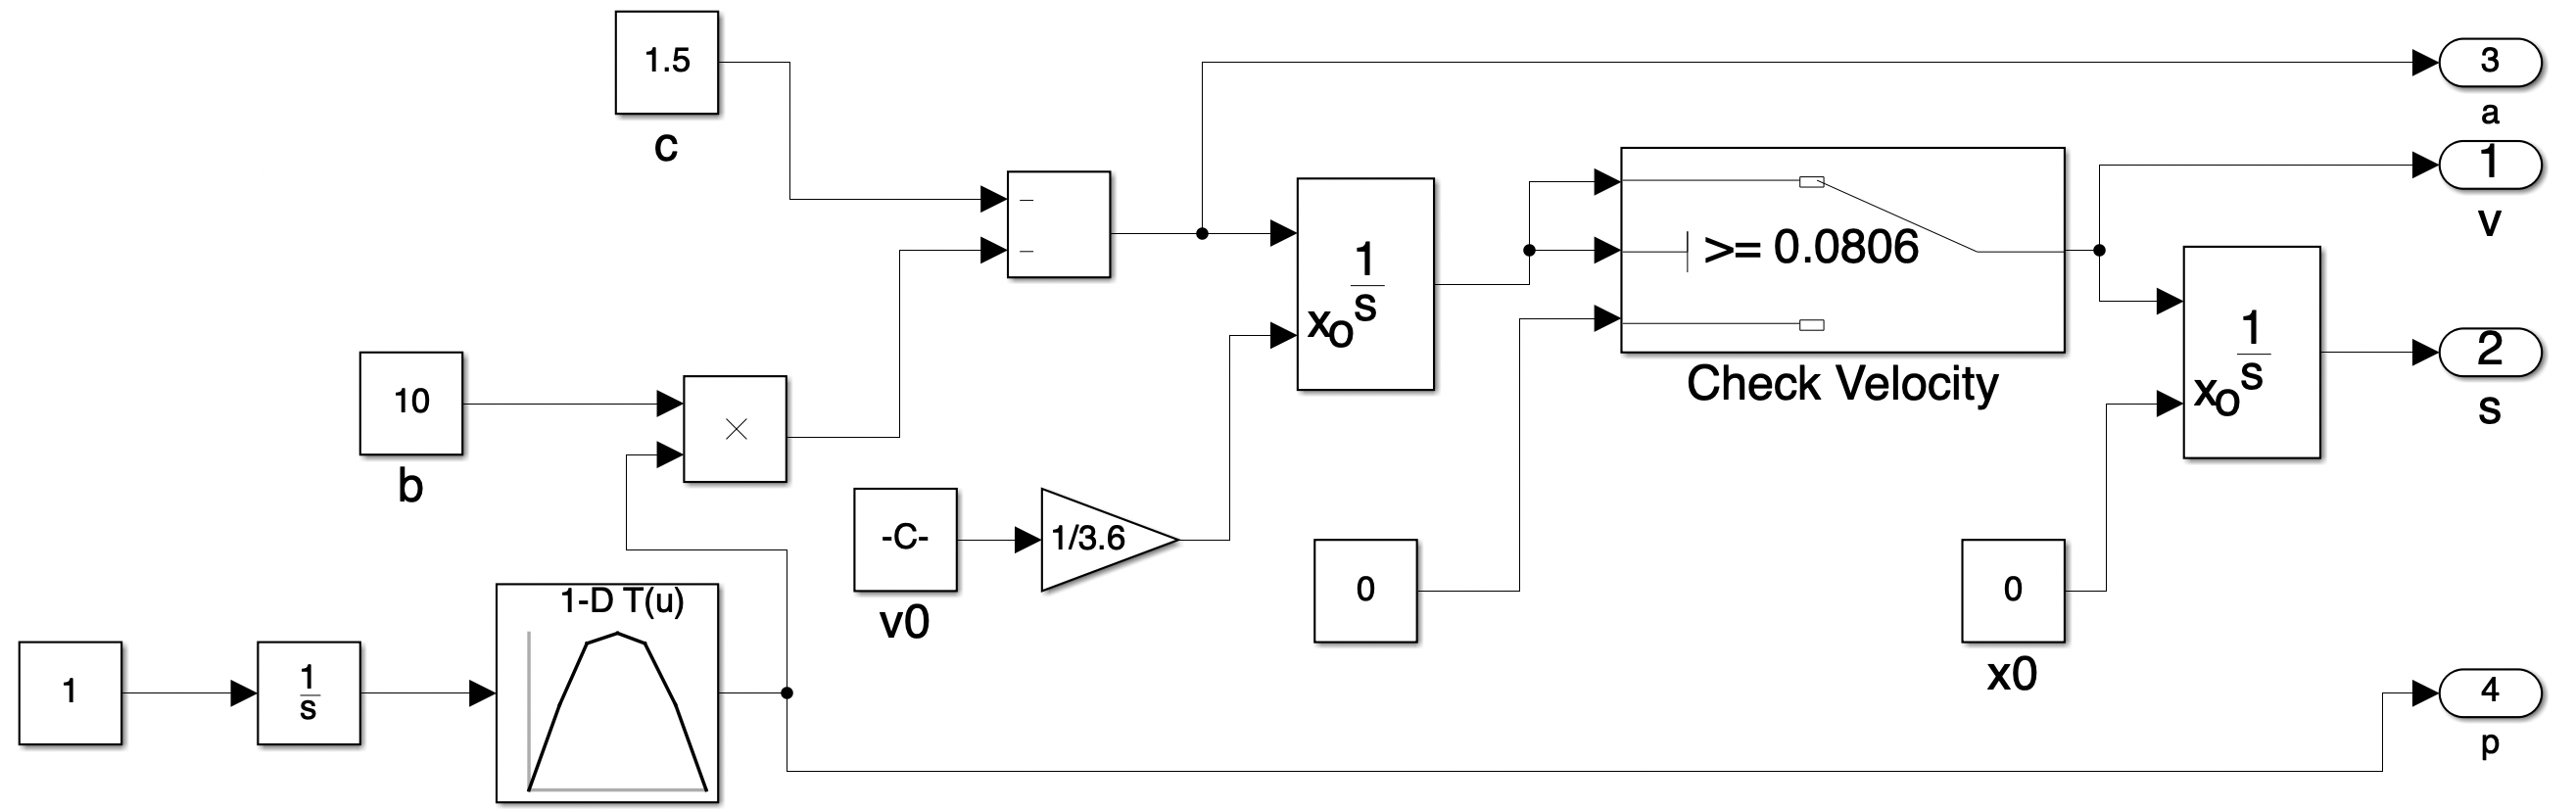
\includegraphics[width=1\textwidth]{images/D3_model_extension.png}
\caption{Simulation without braking}
\label{fig:D3_IndividualBraking2}
\end{figure}
By adjusting the parameters of the lookup-table the following values have been selected to provide smooth human-like braking.
\begin{table}[H]
\centering
\caption{Determined p(t) parameters}
\renewcommand{\arraystretch}{1}
\begin{tabular}{lllllll}
\textbf{Time in [s]} & \textbf{Brake pressure}\\\hline
0 & 0\\
0.2  & 0.043\\
0.4  & 0.073\\
0.6  & 0.078\\
0.8  & 0.073\\
1  & 0.043\\
1.2  & 0\\
\end{tabular}
\end{table}

Figure \ref{fig:D3_pt} shows the results of the Simulink simulation using the parameters from the table above.
With 10 km/h as $v_0$ the car comes to a stop at approximately 1.92 meters.
This leaves a margin for velocity measurement inaccuracies, which will be analysed in chapter \ref{cha:D5} todo check.
The acceleration curve in the third subplot is similar to a human profile, with the exception of the offset of $-1.5\; m/s^2$.
This can not be prevented because there is no gas pedal.
It can also be seen that at the end of the braking procedure at approximately 1.2 s, the brake pedal is released and the friction brings the car to stop.

\begin{figure}[H]
\centering
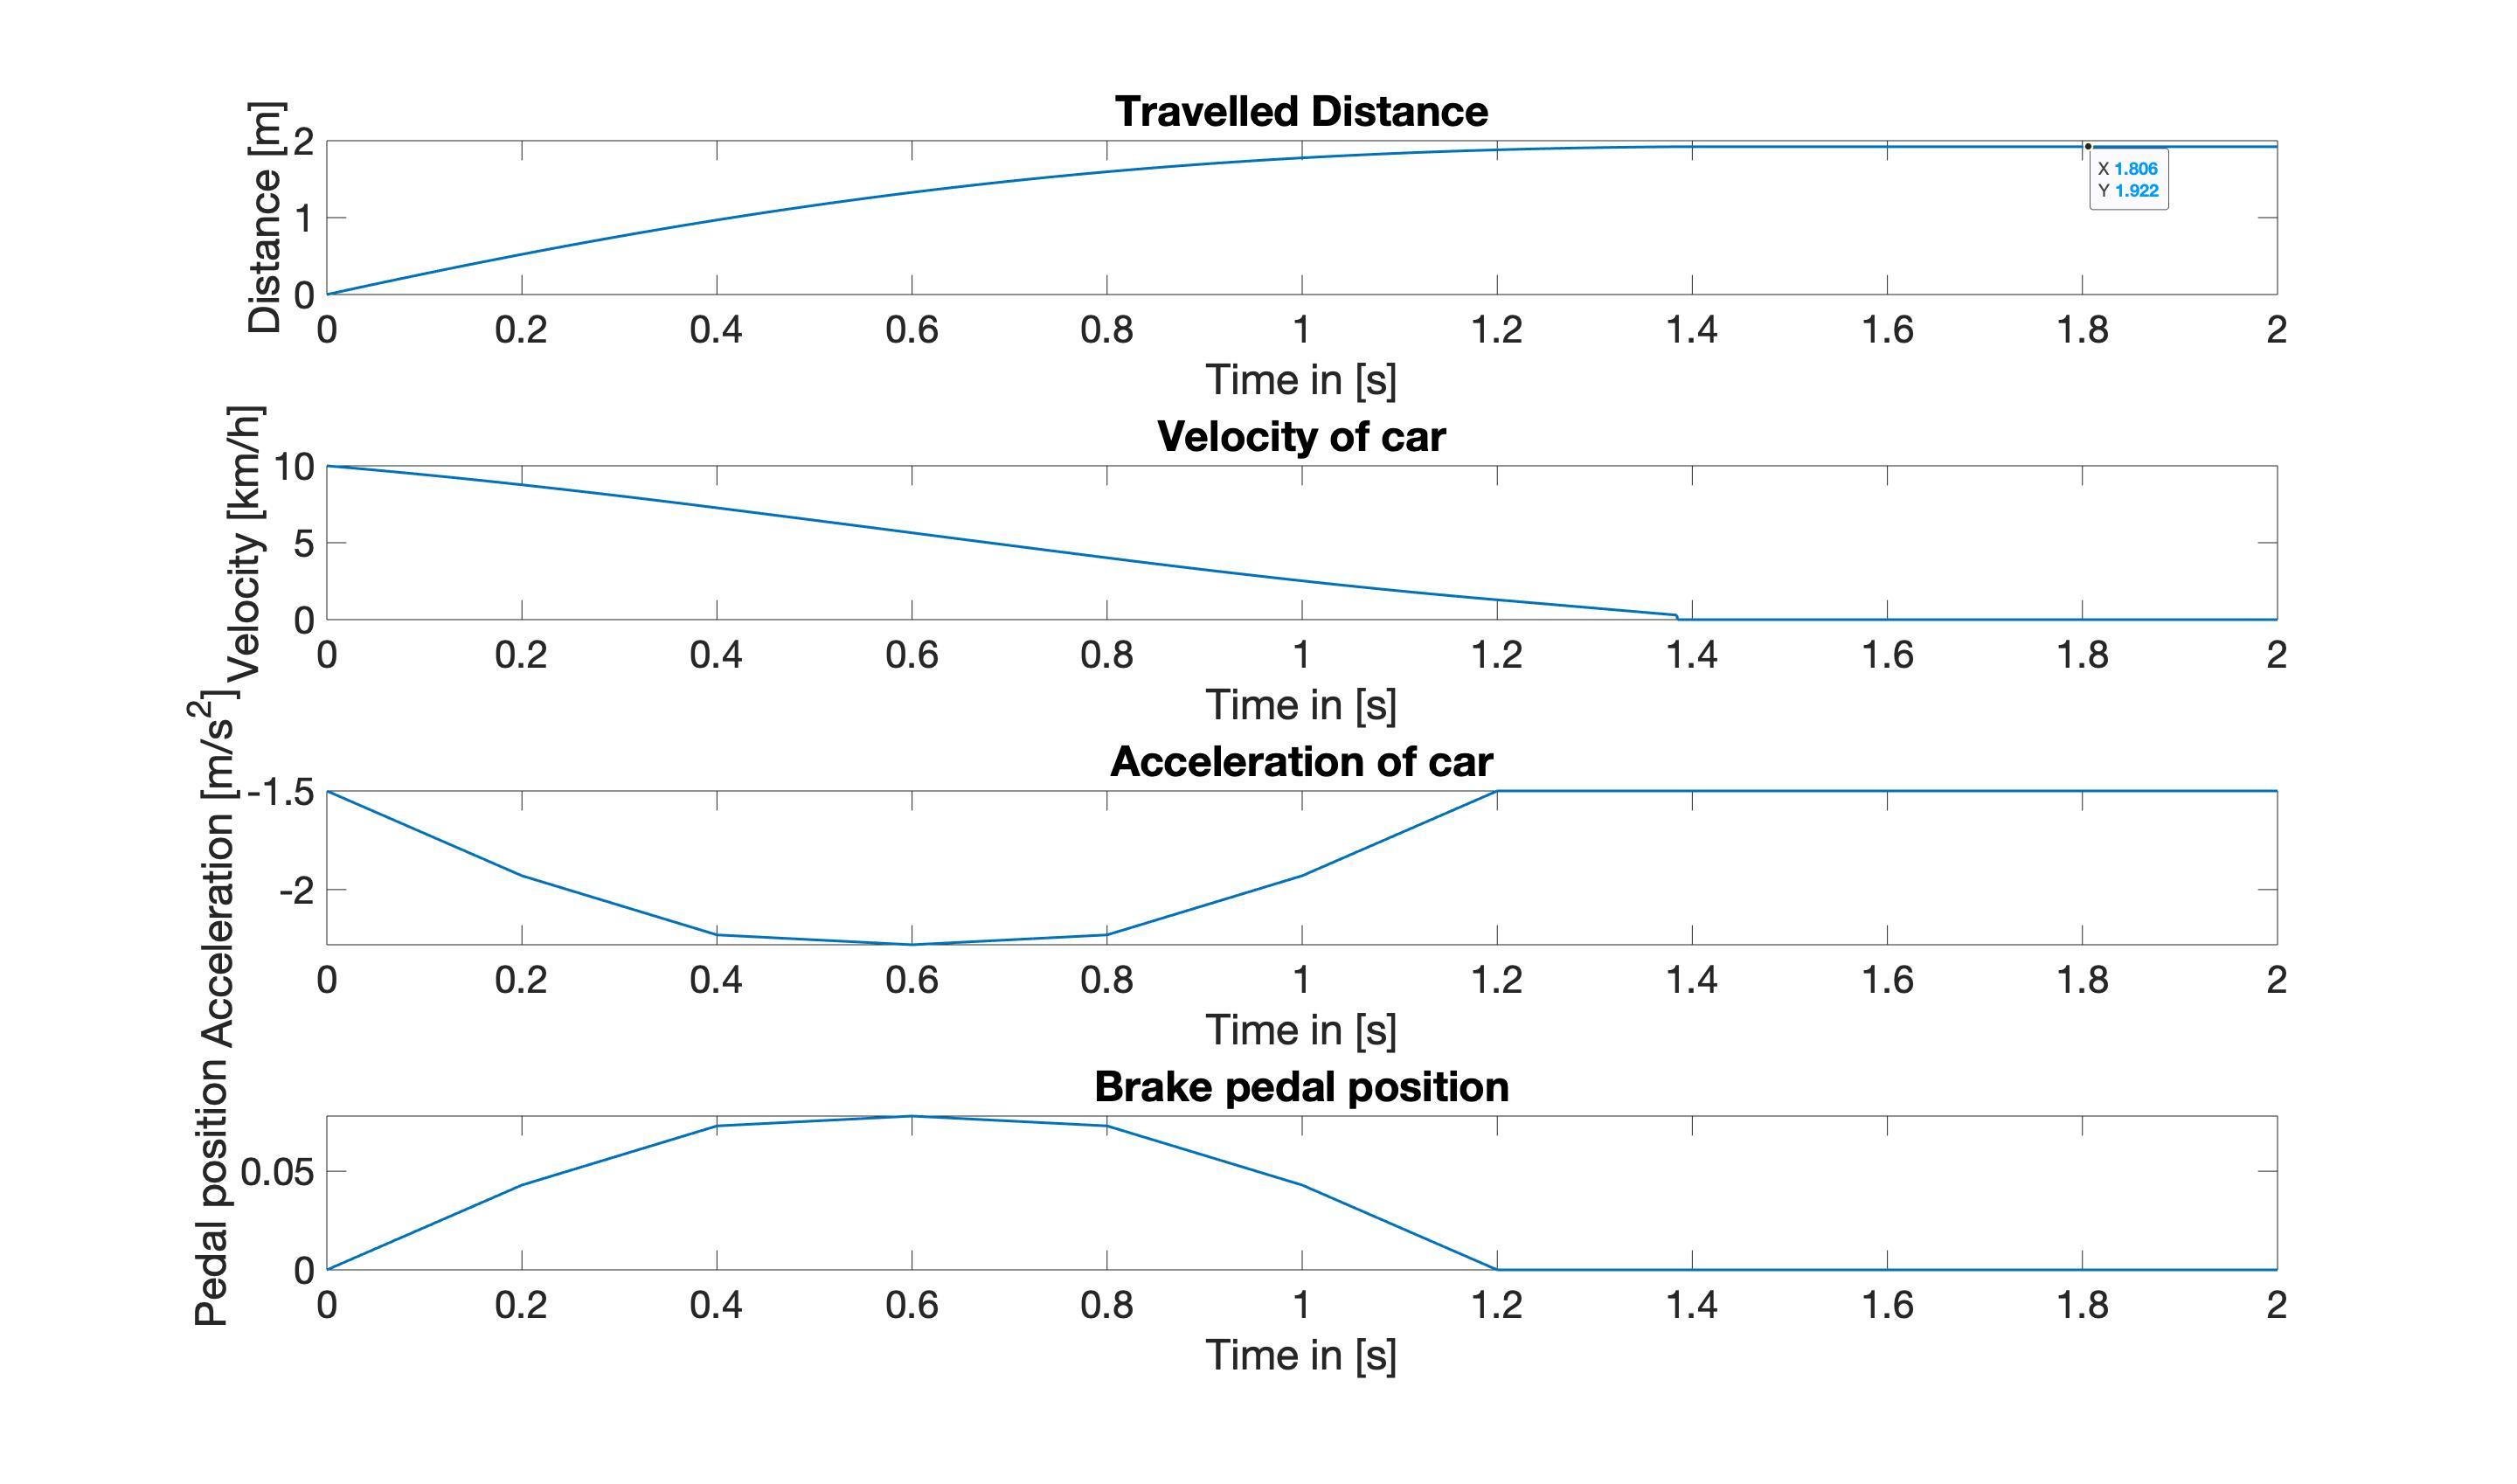
\includegraphics[width=1\textwidth]{images/D3_pt.jpg}
\caption{Simulation results with p(t)}
\label{fig:D3_pt}
\end{figure}

\chapter{D4*: Consideration of uneven parking spaces}\label{cha:D4}

For consideration of uneven parking spaces, the physical car model needs to be expanded to include slope downforce (Hangabtriebskraft).
Also the height profile of the parking space would have to be stored, to be used in the model.
A lookup-table could be used to store the height profile.\\
A negative slope would increase stopping time and position.
A negative slope is critical since a collision could occur.
Depending on the steepness the p(t), that is used now, would not suffice and harder braking would be necessary.\\
A positive slope would make stopping time and location shorter.
This would not lead to a collision, but the car would stop further away from the obstacle.
That could also be not wanted, since then parking space would be used less efficient.\\
If the distance from the obstacle should be the same, regardless of positive/negative slope or even parking space, the brake power needs to be varied depending on steepness. With a negative slope it is needed to brake harder in comparison to an even parking space. With a positive slope lesser braking would be necessary.\\
Depending on $v_0$, with a negative slope, it might not be possible to stop before 2 m of travelled distance.\\
Also after the car is stopped it should not start to roll forwards or backwards.
On a plain surface, the brake can be released, after the car is stopped.
That might not be the case with an uneven parking space and the car could start rolling.
A brake assist on a positive or negative slope would need to keep holding the brake or engaging the handbrake.\\
If the slope is known beforehand (the same as we know now that the parking space is even), that can be included when determining p(t) and adjusting the brake pedal position according to the slope.
Of course the feasibility study (D1) would have to be done again, to determine the feasibility of the task with the changed slope.\\
Also, it does not have to be a solely positive or negative slope.
It could also be first a positive and then a negative slope (or any other height profile) when approaching the parking spot.
For each different slope, a different p(t) would be needed to result in the same stopping position.\\
If the car should be able to stop before 2 m with an unknown slope, a controller with feedback would have to be used instead of p(t), to dynamically adjust the brake pedal position depending on car behaviour.

\chapter{D5: Discussion of inaccuracies in velocity measurement}\label{cha:D5}
\section{Inaccuracy in car velocity}
The velocity information of the car has an inaccuracy of velocity +/- 0.1 km/h.
Also the minimal velocity is 0.29 km/h which is not realistic, because velocity does not drop from 0.29 km/h to zero in one step.\\
The brake pedal function is not dependant on the velocity, therefore inaccuracies in the velocity measurement during the braking procedure do not influence the braking procedure.\\
This has one exception.
Considering the velocity measurement inaccuracy, the initial velocity could be in a range of $9.9\; km/h \leq v  \leq 10.1\; km/h$.
This would certainly influence the braking behaviour of the car.
It would be dangerous if the initial velocity would be higher than expected, because the car would travel further than expected because of that.
This might cause an accident.
If it would be lower, the car might stop earlier but that would not lead to an accident.\\
A simulation is used to evaluate the danger of the initial velocity being higher than expected.
The, highest initial velocity that is possible with R5 is 10.1 km/h.
So this is used as $v_0$ for the impact evaluation.
The model from Figure \ref{fig:D3_IndividualBraking2} from before is used for the evaluation, to see if the margin to 2 m is enough with a $v_0$ of 10.1 km/h.\\
As can be seen from the results of the simulation in figure \ref{fig:D5_results} the margin is enough, since the stopping distance is approximately 1.96 m.
The stopping distance from the correct $v_0$ of 10 km/h (see section \ref{sec:D3_dev_pt}) is 1.92 m. So the velocity difference of 0.1 km/h results in a stopping distance difference of circa 4 centimeters.

\begin{figure}[H]
\centering
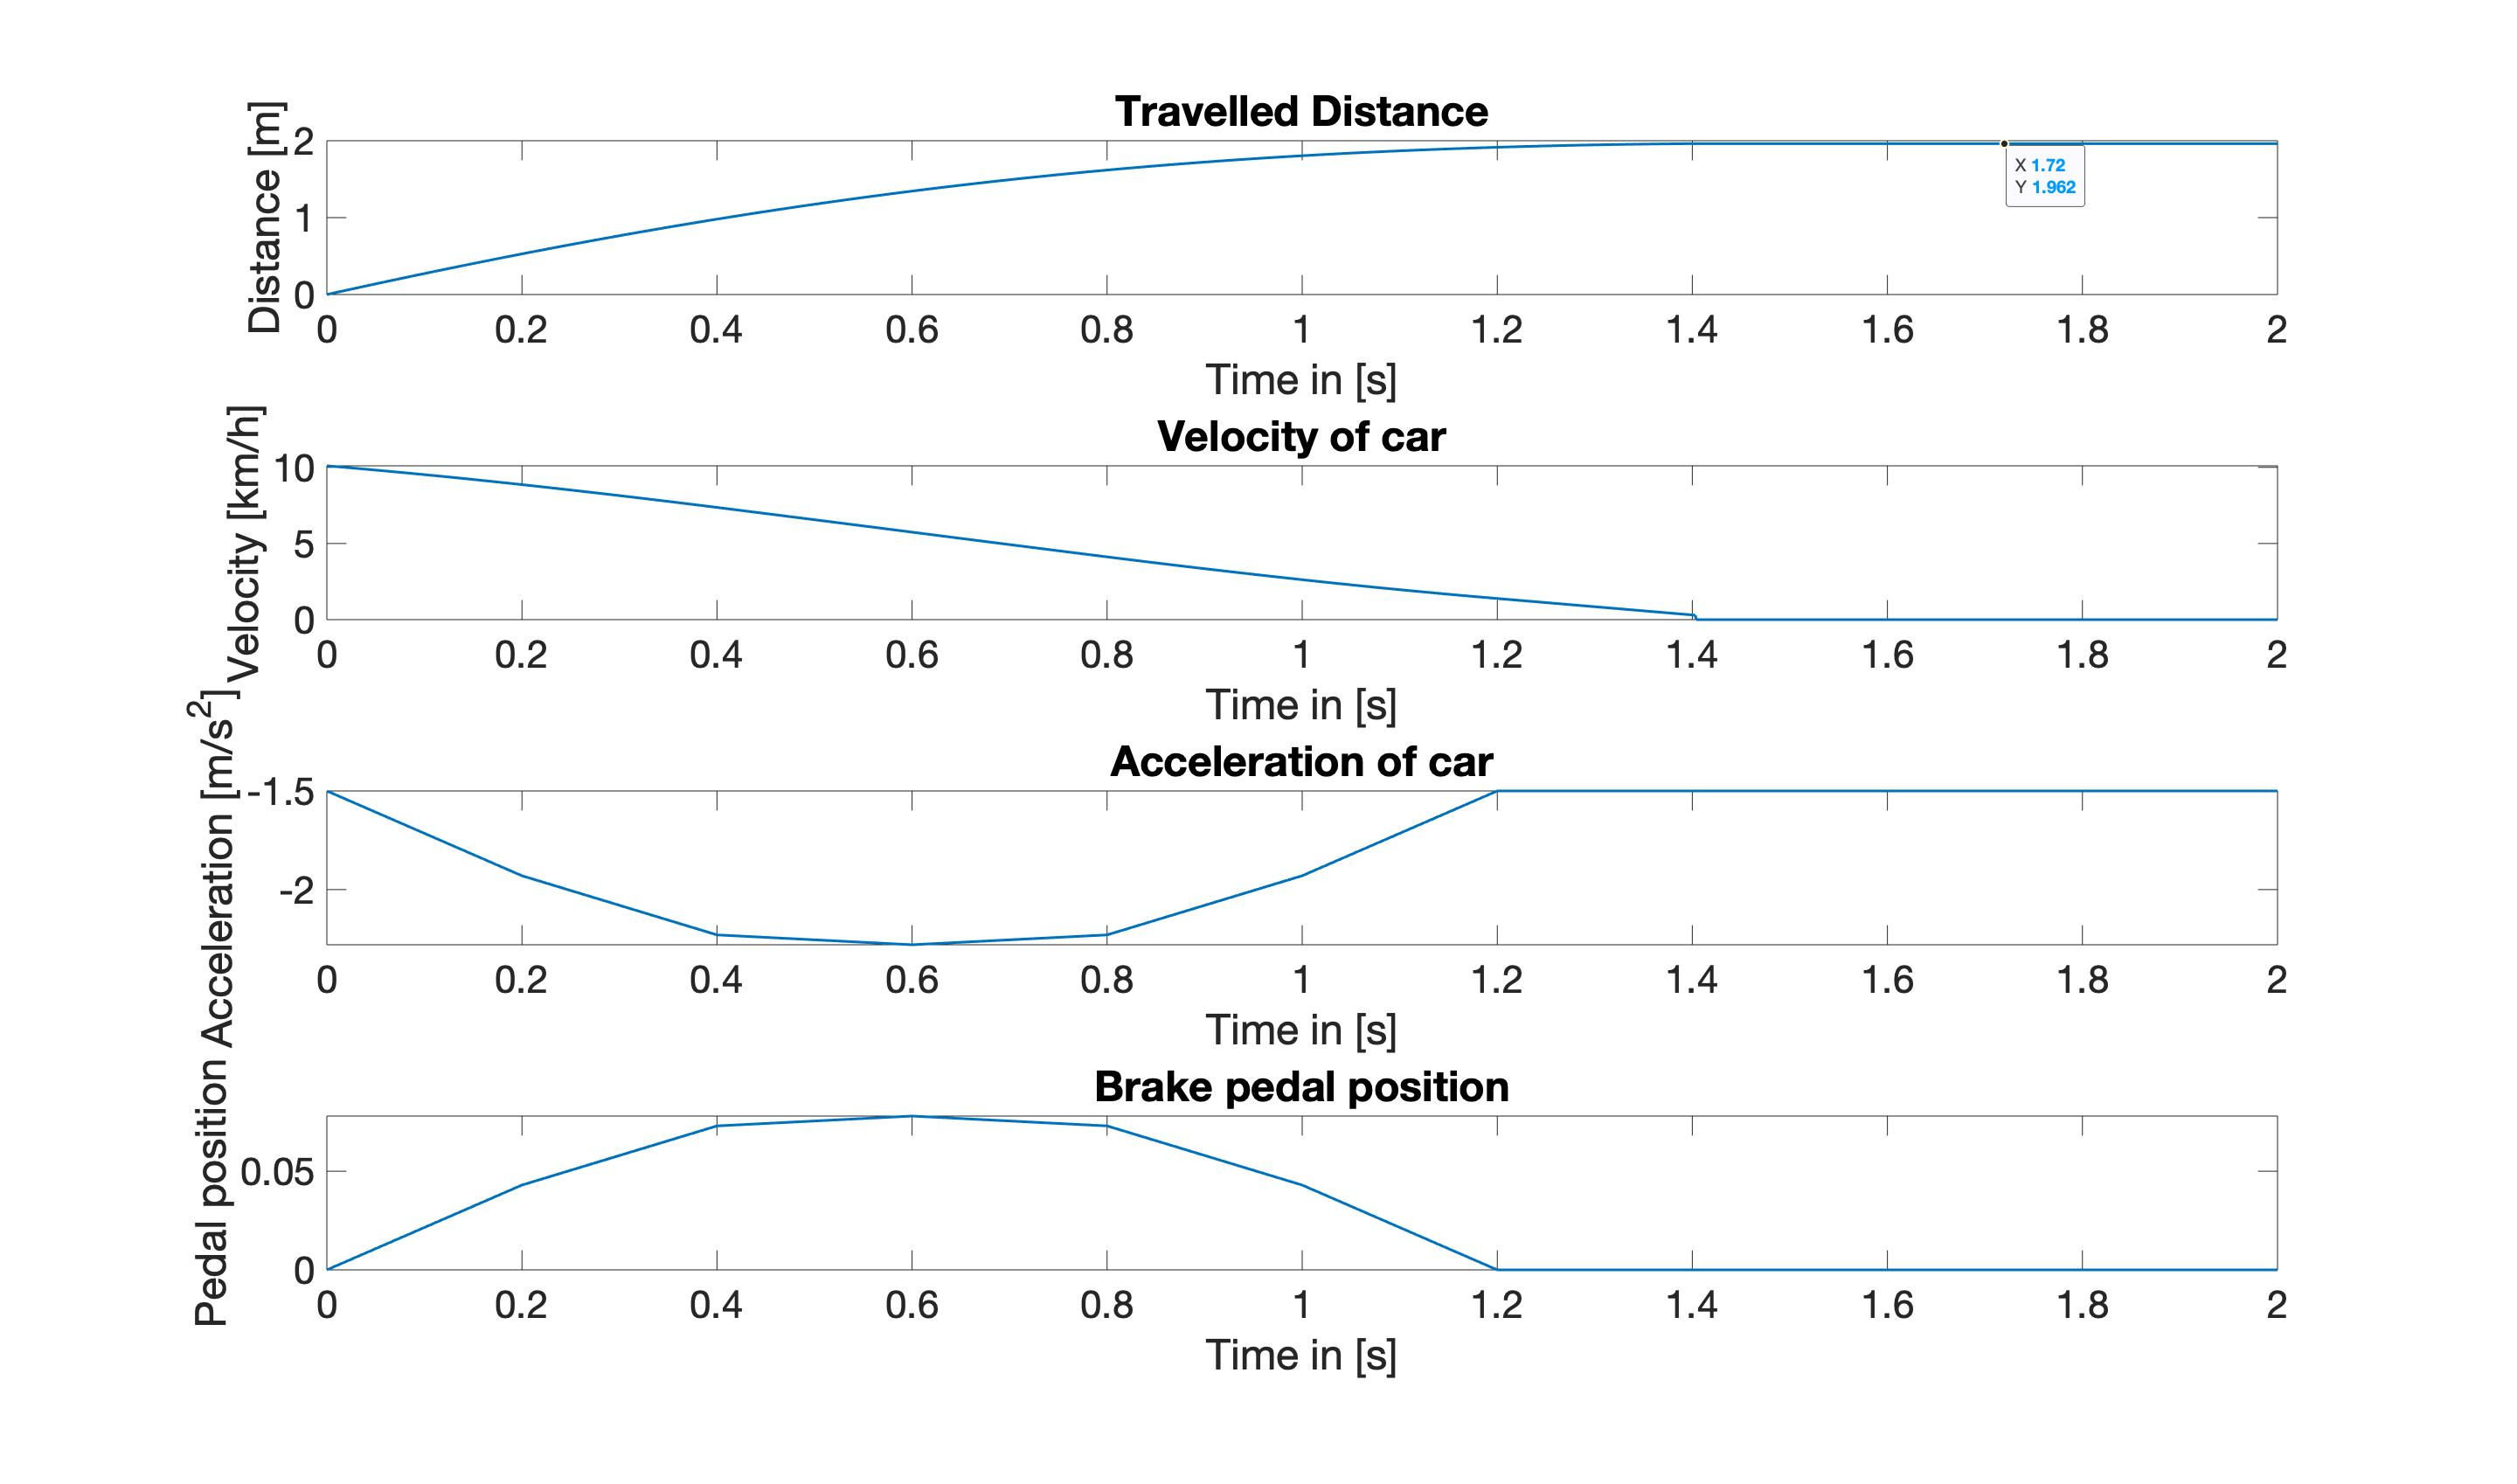
\includegraphics[width=1\textwidth]{images/D5_result.jpg}
\caption{Simulation of inaccurate $v_0$}
\label{fig:D5_results}
\end{figure}

Uncertanties in the measured velcoity also influence the computed travelled distance.
The velocity is needed to compute the travelled distance. The travelled distance is computed as the integral of the velocity. Therefore errors in the velocity accumulate in travelled distance.\\
However if the error follows a gaussian distribution, the integrated error would be relatively small, because over- and under-estimation would be equally likely.

\section{Inaccuracy in velocity measurement of human velocity profile}
In the human velocity profile 4 tire velocities are recorded.
To estimate the car velocity the mean of the 4 wheel velocities has been computed.
It was assumed, that the car is moving in a straight line and not going around corners.\\
Also the minimal velocity in the recorded measurement data is 0.29 km/h.
Therefore the braking behaviour below this threshold can not be analysed.\\
The inaccuracies in the measured velocity also influence the computed acceleration.
The acceleration that has been computed by time-discrete differentiation from the measured velocity is only an estimate and not the real acceleration during recording.\\
In chapter \ref{cha:D3} (D3) a moving averaging filter has been used to smoothen the data and reduce the measurement noise.


\chapter{D6: Implementation of pulse signal in Simulink}\label{cha:D6}

In D6 a pulsing information signal is described. This chapter documents the implementation of that signal.
Both signals are needed for the frequency computation.
The pulsing signal should only be present if the nonzero velocity of the car is $\leq$ 1 m/s and the position of the car is between 1 and 2 meters. From a frequency of 1 Hz at 1 meter it should rise up to 9 Hz at 1.9 meters. If the traveled distance is greater than 1.9 meters, the signal should become continuous.\\
This requirement can be divided into two separate compontents with separate responsibilities.\\
In the first component it is determined in which state the signal is (off, pulsing, continuous) and in the case of a pulsing signal the frequency of that pulse is computed.\\
The second component is responsible for outputting the pulse signal corresponing to the output of the first component.\\
The components are implemented using simulink subsystems which enables re-usability, encapsulation and also creates a better overview when looking at the main simulink model.\\
\section{Computation of pulse signal frequency}\label{sec:D6Frequency}
Figure \ref{fig:D6_Frequency_Computation} shows the simulink subsystem for the computation of the frequency of the pulse signal.
The inputs are the velocity and position of the car.
The if-condition determines in which state the signal is.\\
In the first case the nonzero car velocity is $\leq$ 1 m/s and the position of the car is $>$ 1.9 meters.
In this case, the pulsing signal should provide a continuous output as demanded by requirement D6.
The subsystem outputs a value of 10 in that case.
This value is the indication for a continuous signal.\\
In the second case of the if condition the nonzero car velocity is also $\leq$ 1 m/s but the position of the car is between 1 and 1.9 meters.
In this case the frequency of the pulsing signal should be between 1 and 9 Hz depending on the location.
For that a lookup table is used, that provides an output frequency that linearly increases from 1 to 9 Hz depending on the position from 1 to 1.9 meters. A linear increase is used, because then the driver could estimate the position linearly by the signal.\\
When none of the above mentioned conditions are the case, the subsystem outputs 0, which indicates that the pulsing signal is not present.

\begin{figure}[H]
\centering
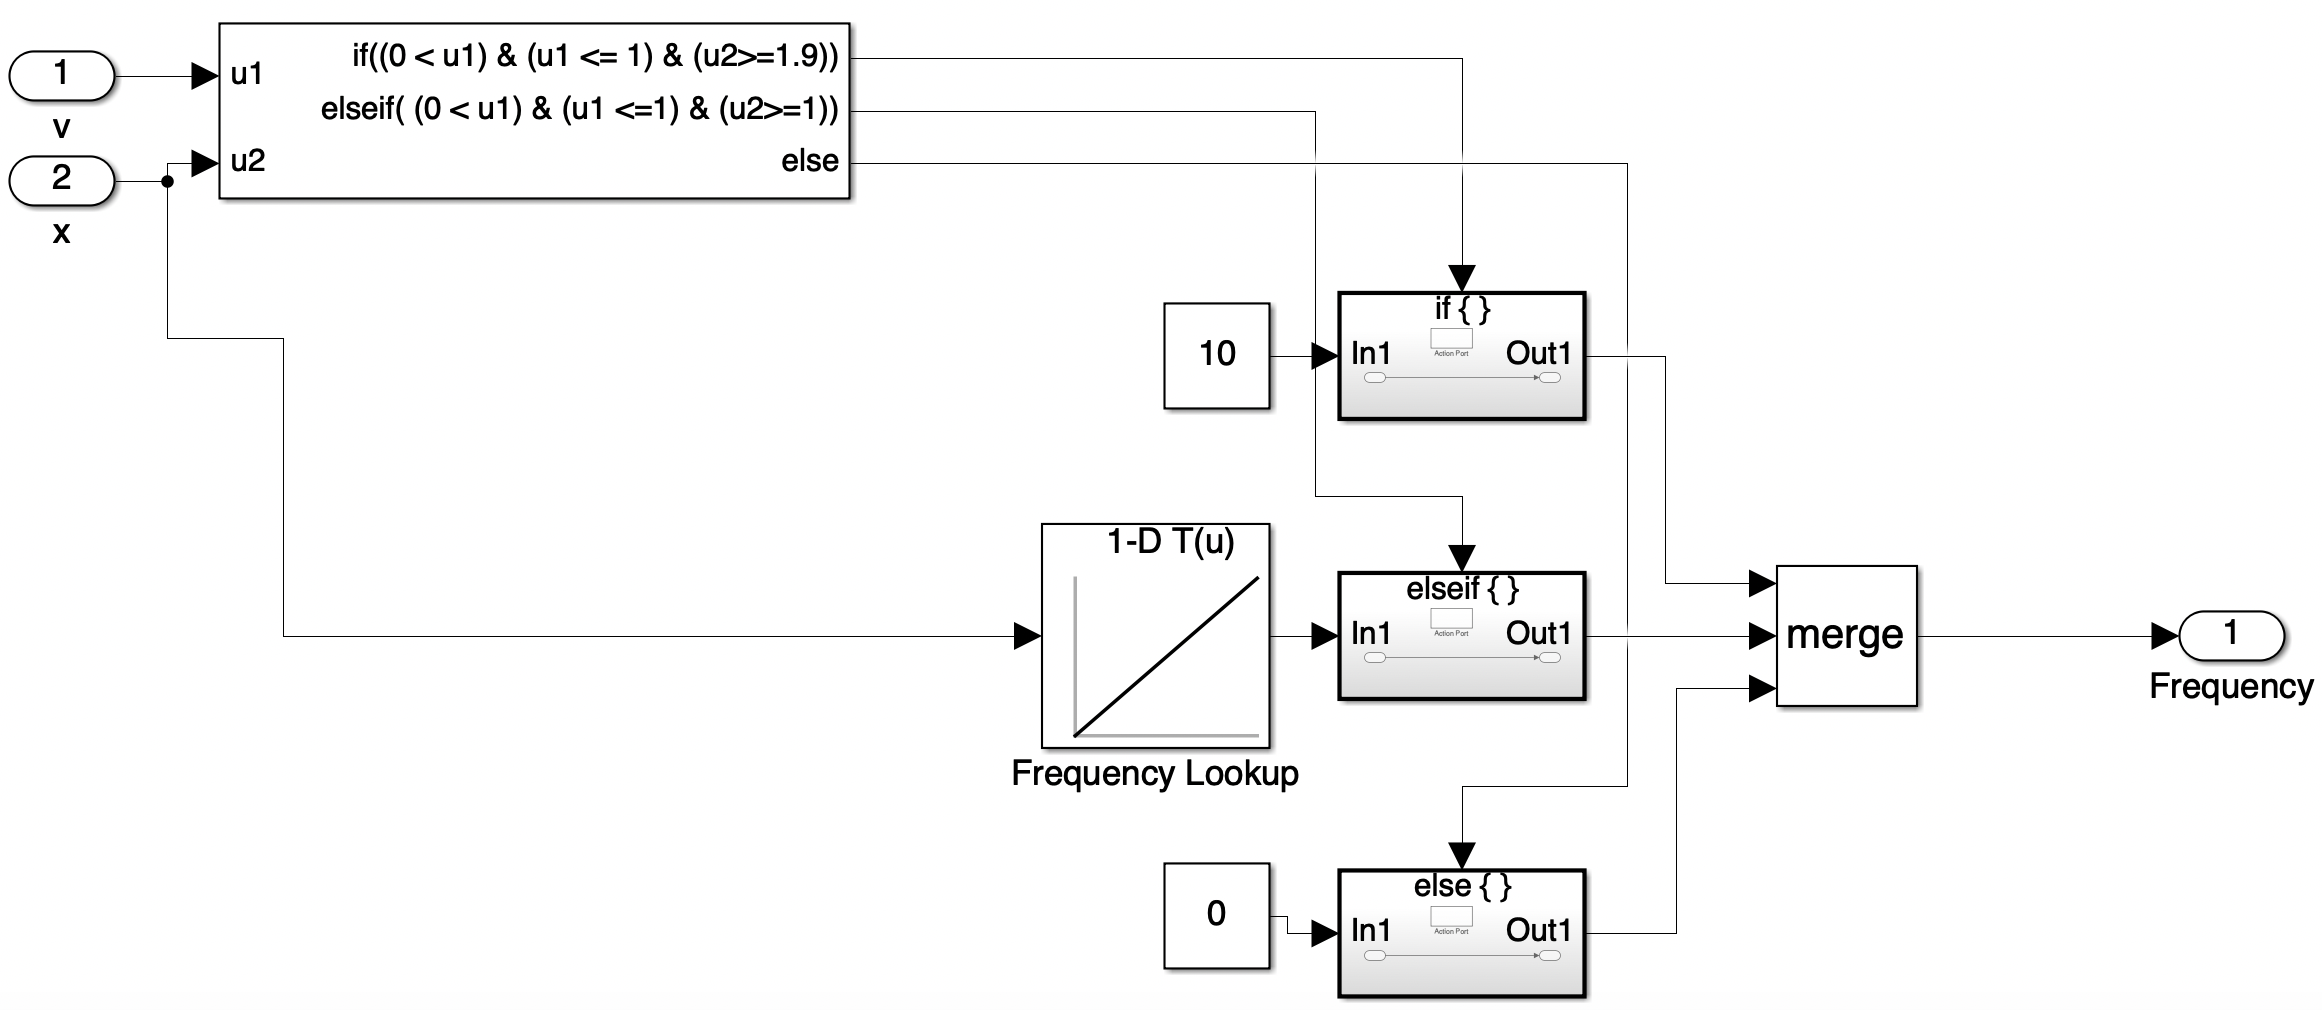
\includegraphics[width=1\textwidth]{images/D6_Frequency_Computation.png}
\caption{Simulink model of the frequency computation subsystem}
\label{fig:D6_Frequency_Computation}
\end{figure}

\section{Pulse signal generation}\label{sec:D6Signal}
Figure \ref{fig:D6_Pulse_Signal} shows the simulink model of the pulse signal generator.
This component provides a pulse signal with a variable frequency input.
The input is the output of the before described component.
Therefore if the input is 10, a continuous signal should be output.
This is realised by the if-condition, which, if the input signal is 10 provides a continuous high output.\\
If the frequency is 0, 0 should be output.\\
If that is not the case either the pulse signal is generated.
The frequency is the input to the integrator.
The integrator has a reset input port and will be reset after each period.
For each period the output of integrator will start at 0 and will go up to 1.
Until the output reaches 0.5 a high pulse will be output (50 \% duty cycle).
This is the purpose of the less or equal 0.5 check.
If the output of the integrator is greater that 0.5 a low pulse is output.

\begin{figure}[H]
\centering
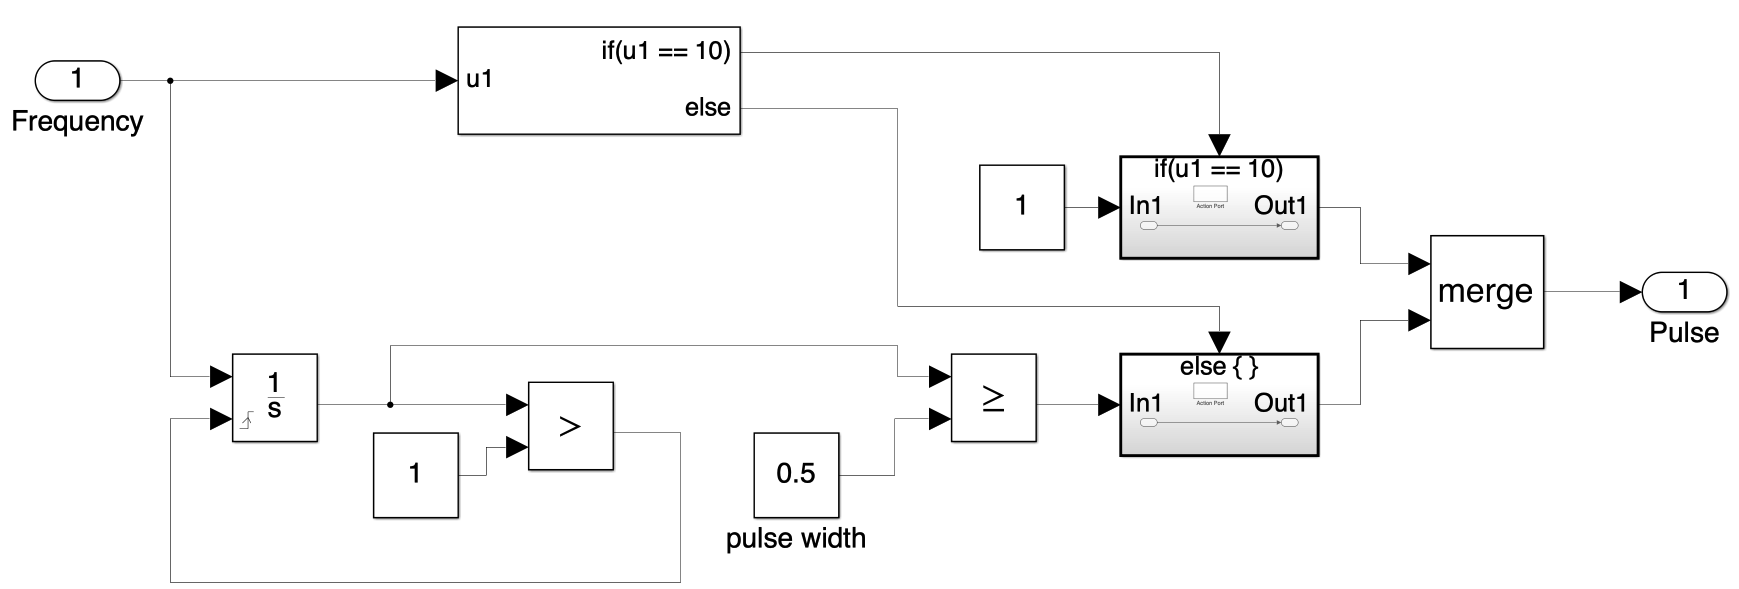
\includegraphics[width=1\textwidth]{images/D6_provide_signal.png}
\caption{Simulink model of the pulse generation subsystem}
\label{fig:D6_Pulse_Signal}
\end{figure}

\section{Integration into car model}\label{sec:D6Frequency}
Using subsystems for the developed components makes it easy to include into and extend the existing model, which can be seen in figure \ref{fig:D6_Integation}. We have integrated it into the model from chapter \ref{cha:D2}, because p(t) is not needed for the pulse signal demonstration. Integrating the pulse signal into the model from section \ref{sec:D3_dev_pt} would follow the same procedure.
\begin{figure}[H]
\centering
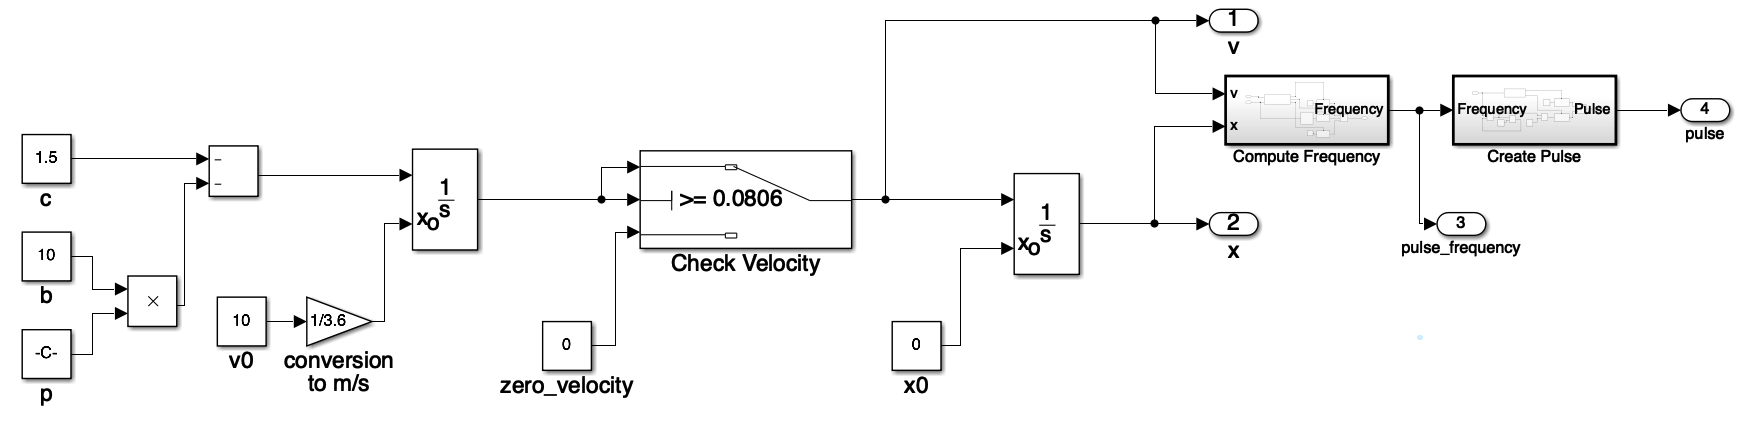
\includegraphics[width=1\textwidth]{images/D6_integration.png}
\caption{Simulink model of the car including the pulse signal}
\label{fig:D6_Integation}
\end{figure}

\section{Signal demonstration}\label{sec:D6_SignalDemonstration}
Figure \ref{fig:D6_Result} shows a demonstration of the implemented pulse signal. The Simulink car model is initialised with a constant brake pressure of 5 \%. The frequency computation functionality can be seen in subplot 3. The frequency rises from zero, when the car reaches a velocity of 1 m/s (and also the distance is greater than 1m). Then the frequency increases as the car moves closer to 2 m. At 1.9 m traveled distance, the frequency rises to 10, which indicates a continuous pulse. When the car comes to a full stop at approximately 1.4 seconds the frequency goes back to zero, which indicates no pulse. The fourth subplot shows the output pulse signal. It starts when the frequency rises from zero, and the period of the pulses gets shorter with the time increasing. When the frequency starts to indicate a continuous pulse (from approximately 1.25 s) the pulse signal outputs a continuous high signal until the car comes to a stop. When the car stops, the continuous pulse stops and no pulse is output.

\begin{figure}[H]
\centering
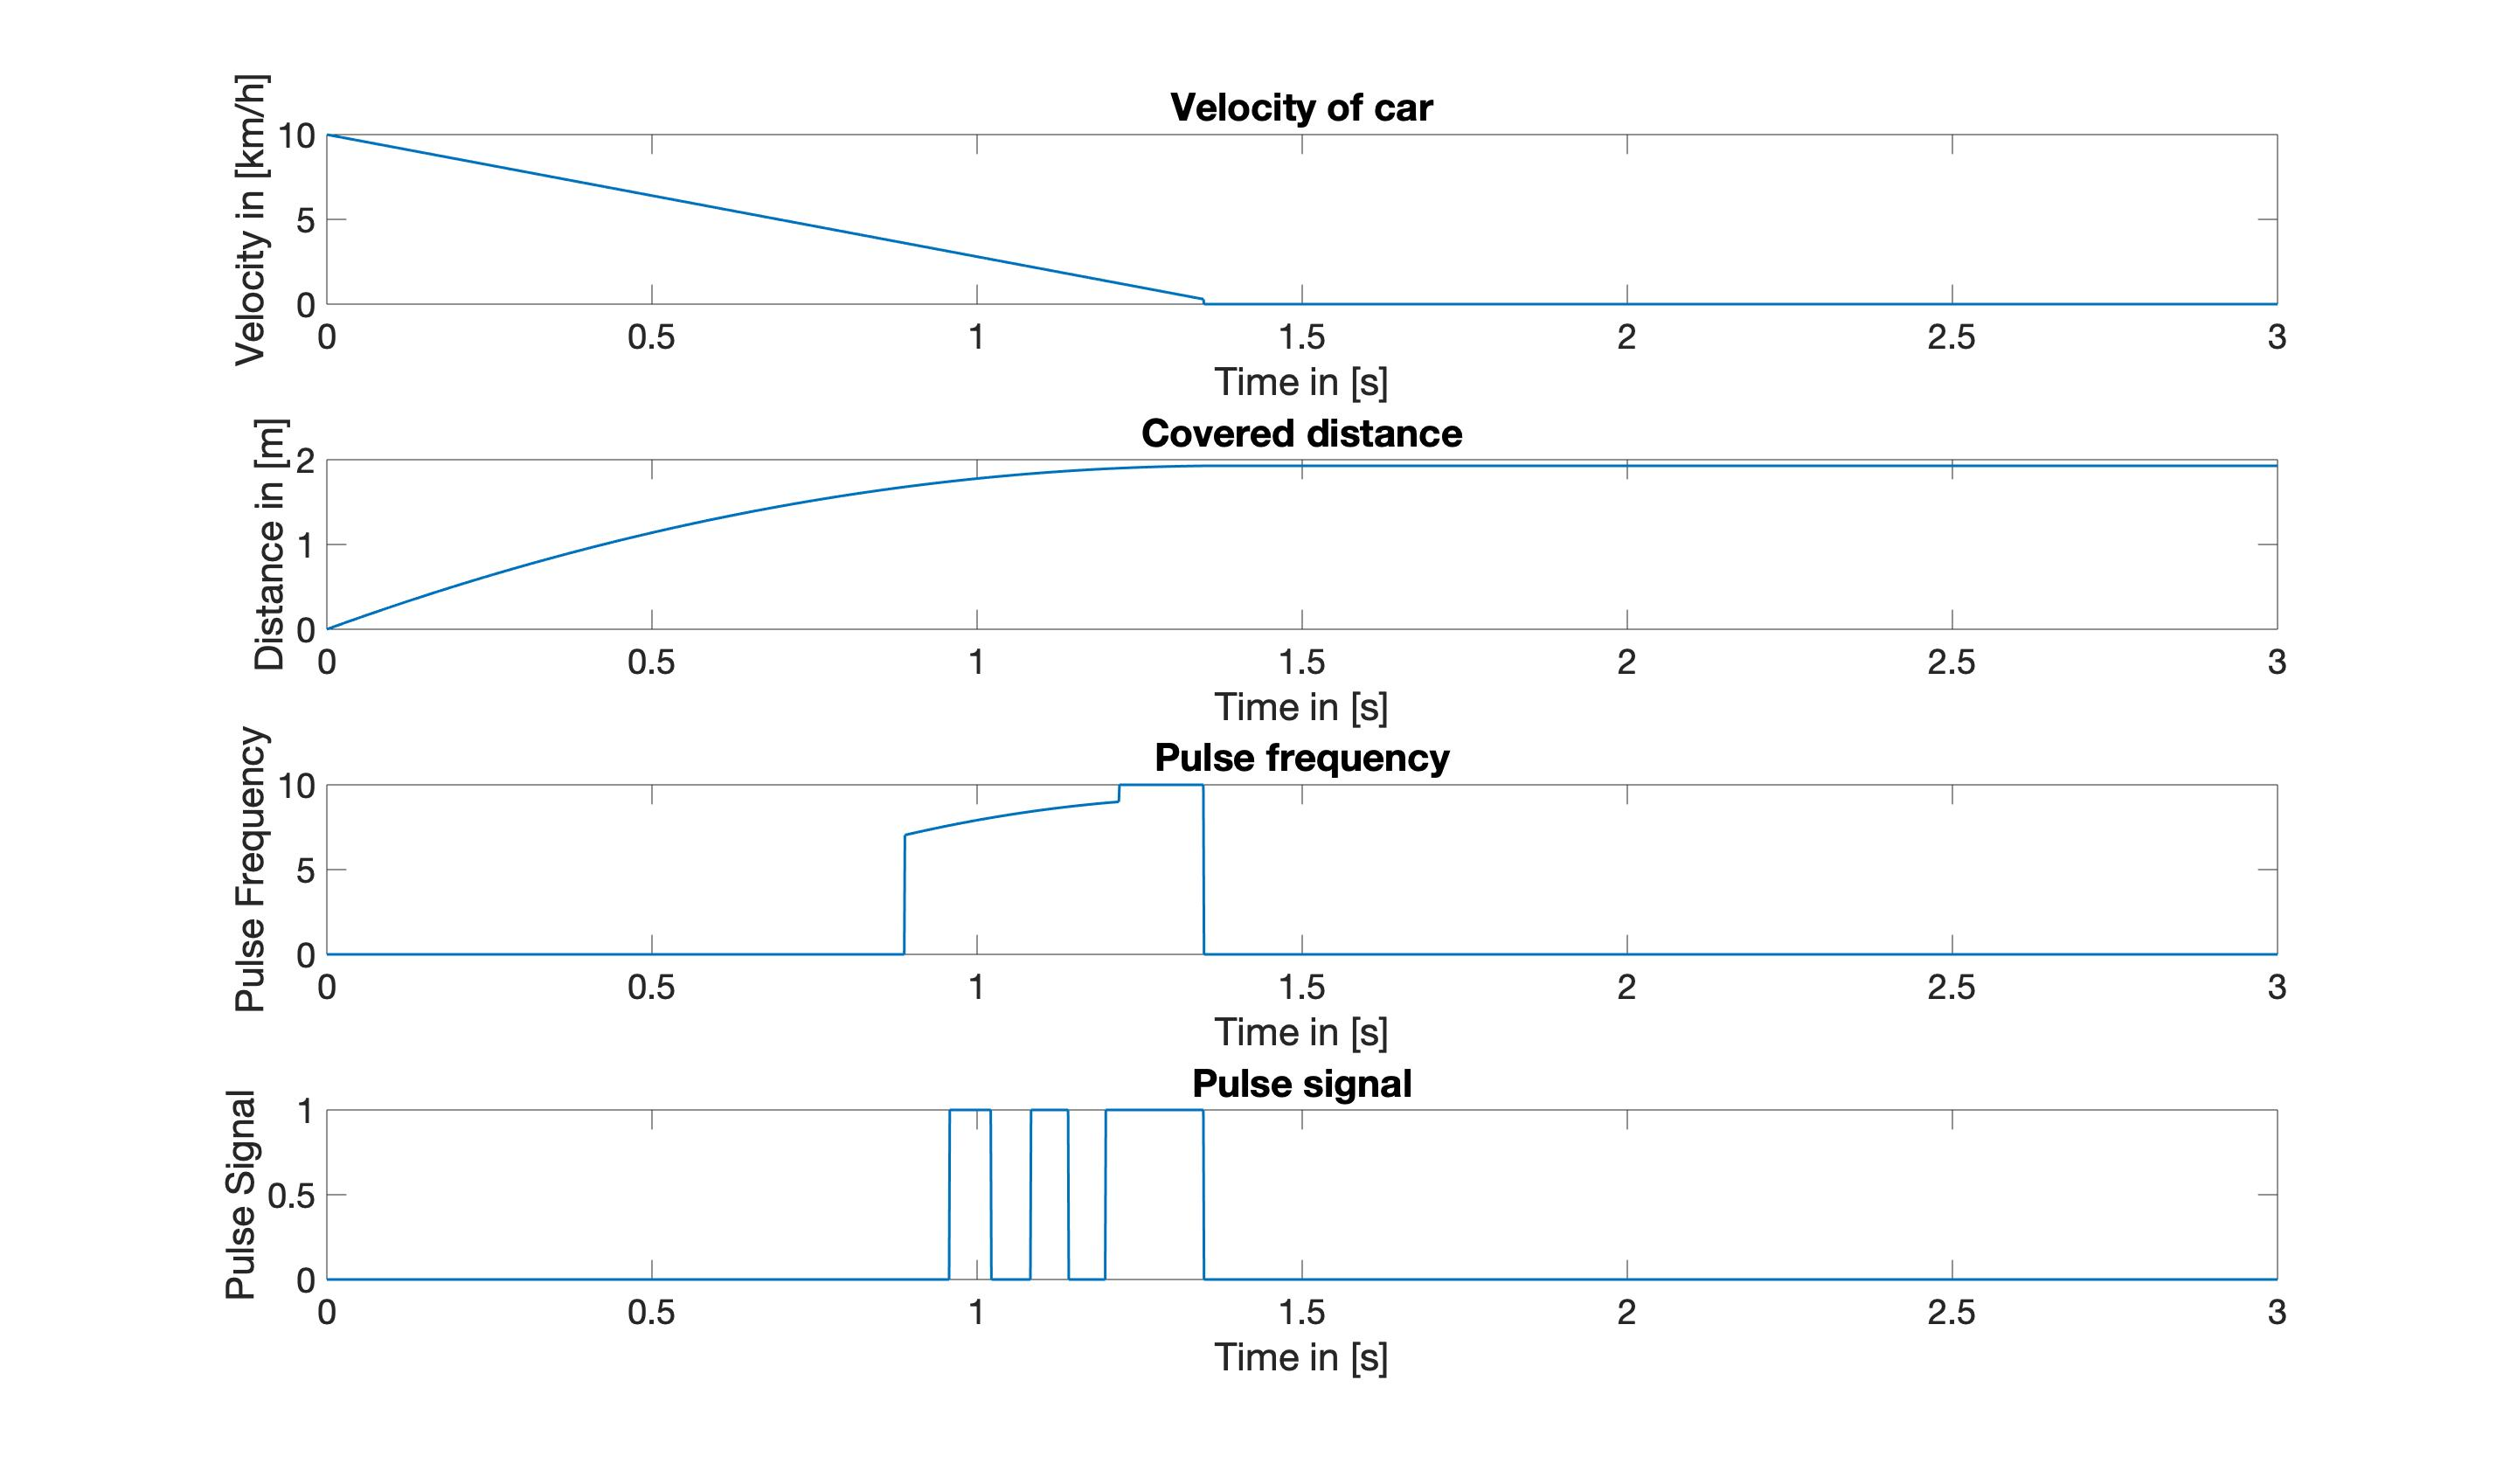
\includegraphics[width=1\textwidth]{images/D6_result.jpg}
\caption{Demonstration of pulse signal}
\label{fig:D6_Result}
\end{figure}

\chapter{D7: Transfer of Simulink model to ASCET}\label{cha:D7}

This chapter describes how the Simulink model from section \ref{sec:D3_dev_pt} is transferred to ASCET (and the ultrasonic distance is added).
Furthermore, as ASCET is time discrete execution slots for threads are defined.

First, messages are defined to describe the needed data interfaces. Listing \ref{lst:D7_Messages} shows the two defined message interfaces. The first interface represents messages regarding the car including its velocity, its acceleration, its position, the ultrasonic distance and the pulse signal. The other interface contains a message that describes the current brake pedal position.

\begin{lstlisting}[language=Java,basicstyle=\scriptsize, caption= Defined messages in ASCET,label= lst:D7_Messages]
data interface CarMessages {
	real v = 0.0;
	real acceleration = 0.0;
	real position = 0.0;
	real ultrasonic_distance = 0.0;
	real pulse_signal = 0.0;
}

data interface ParkAssistMessages {
	real brake = 0.0;
}
\end{lstlisting}

The car model is built using the static class $Car$ whose block diagram is shown in Figure \ref{fig:BlockdiagrammCar}. The class consists of three thread functions: $drive$, $velocity$ and $ultrasonic$. The $drive$ function reads the brake pedal message and passes it together with a time constant to an instance of the $DriveModel$ class (shown in Figure \ref{fig:BlockdiagrammDrivingModel}). Consequently, the function writes the acceleration message based on the $DriveModel$ class output. The $velocity$ function writes the v message and the position message. The $ultrasonic$ function writes the ultrasonic\textunderscore distance message. The functionality of the $Car$ class is split in three thread functions because of the given requirements demand the ultrasonic\textunderscore distance to be available every 2ms and the velocity to be available every 10ms. The implemented functions can be called individually in the specified time intervals.

\begin{figure}[H]
\centering
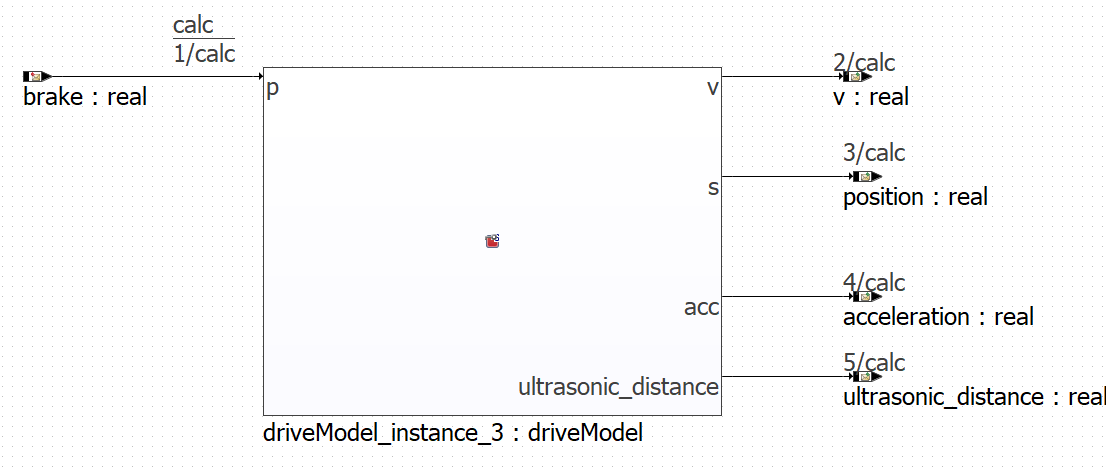
\includegraphics[width=1\textwidth]{images/Blockdiagramm_car.png}
\caption{ASCET block diagram of static class $Car$}
\label{fig:BlockdiagrammCar}
\end{figure}

The $DriveModel$ class is responsible for calculating the acceleration, velocity and position of the car as well as the ultrasonic distance.
These calculations are based on the input brake pedal position.
The block diagram of the class is shown in Figure \ref{fig:BlockdiagrammDrivingModel}.
Similar to the Simulink model, the acceleration is calculated by multiplying brake pedal position and the braking constant and substracting it from the negative friction constant. The velocity is calculated by integrating the acceleration.
Unlike Simulink ASCET is time-discrete, so acceleration, time constant and the factor 3.6 to convert the acceleration from [m/s] to [km/h] are multiplied to compute the velocity change. The product is then added to the previous velocity. The default velocity is set to 10 km/h due to the requirements (as default value in the v variable). If the velocity is less than 0.29 km/h it is set to zero based on requirement R5. The position is obtained by multiplying velocity and time constant and diving it by 3.6 to get the position in meters and not in kilometres. The product is then also being added to the previous position whose default value is zero. The ultrasonic distance is gained by subtracting target position (2m) and position.

\begin{figure}[H]
\centering
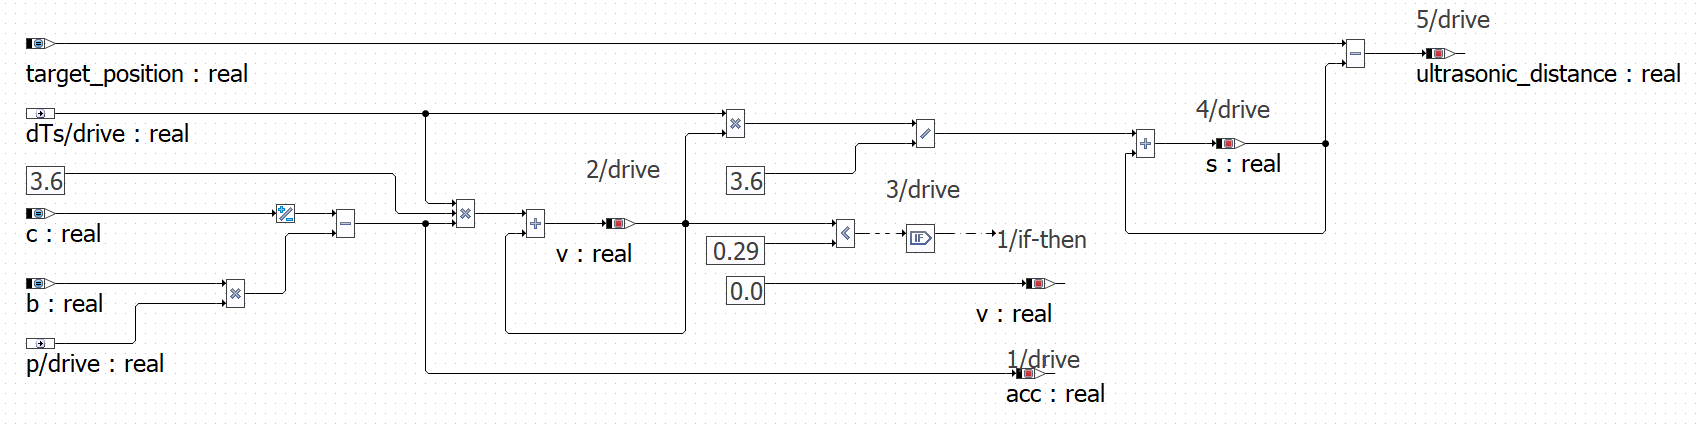
\includegraphics[width=1\textwidth]{images/Blockdiagramm_drivingmodel.png}
\caption{ASCET block diagram of class $DriveModel$}
\label{fig:BlockdiagrammDrivingModel}
\end{figure}

The static class $ParkAssistController$ (see Figure \ref{fig:BlockdiagrammParkAssistController}) is implemented for generating the brake pedal position. Based on the elapsed time since starting the experiment, the class uses an instance of the class $ParkAssistControllerClass$ to generate the brake pedal position and writes the brake pedal message afterwards. 

\begin{figure}[H]
\centering
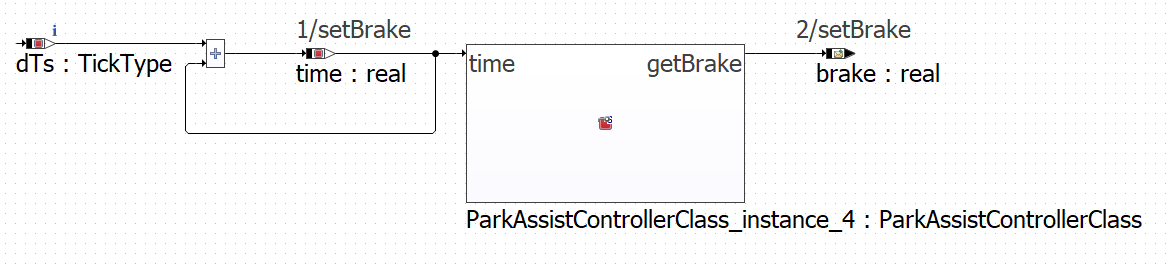
\includegraphics[width=1\textwidth]{images/Blockdiagramm_ParkAssistController.png}
\caption{ASCET block diagram of static class $ParkAssistController$}
\label{fig:BlockdiagrammParkAssistController}
\end{figure}

The brake pedal position is determined based on a look-up table that represents the brake pedal function described in section \ref{sec:D3_dev_pt}. After determining the brake pedal position, the position is returned.  The class $ParkAssistControllerClass$ is implemented as a non static class in order to unit test the class. The block diagram of the class is shown in Figure \ref{fig:BlockdiagrammParkAssistControllerClass}. 

\begin{figure}[H]
\centering
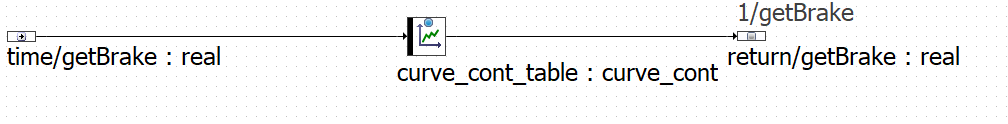
\includegraphics[width=1\textwidth]{images/Blockdiagramm_ParkAssistControllerClass.png}
\caption{ASCET block diagram of class $ParkAssistControllerClass$}
\label{fig:BlockdiagrammParkAssistControllerClass}
\end{figure}

The brake pedal position look-up table is shown in Listing \ref{lst:D7_lookup}. 

\begin{lstlisting}[language=Java,basicstyle=\scriptsize, caption= Braking pressure look up table,label= lst:D7_lookup]
characteristic curve_cont curve_cont_table = {{0.0, 0.2, 0.4, 0.6, 0.8, 1.0, 1.2}, {0.0, 0.043, 0.073, 0.078, 0.073, 0.043, 0.0}};
\end{lstlisting}

In order to execute the experiment, it is necessary to define the scheduling. As can be seen in Figure \ref{fig:D7_schedule}, the experiment is divided in two tasks, one being executed every 2ms and the other task being executed every 10ms. As defined in requirement R4, the ultrasonic distance message is computed every 2ms. Alongside this, the ParkAssistController adjusts the brake pedal position and the pulse signal is computed also every 2ms for a higher precision. The velocity however is generated every 10ms as described in requirement R5. Furthermore, the check for the $SystemTestEnvironment$ (see chapter \ref{cha:D10}) is executed every 10ms as this is precise enough for the check because mainly the end result is of interest.
 
\begin{figure}[H]
\centering
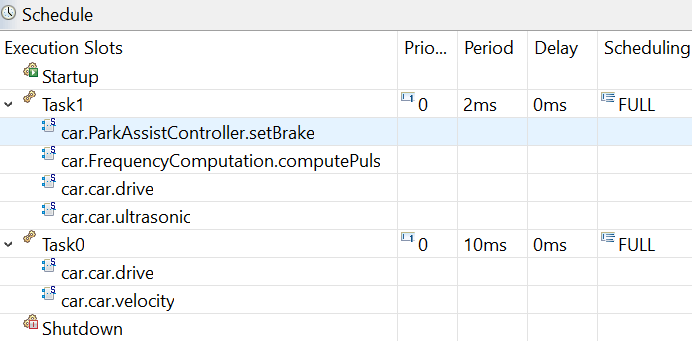
\includegraphics[width=1\textwidth]{images/pc_app.png}
\caption{Scheduling of ASCET model}
\label{fig:D7_schedule}
\end{figure}

The following Figure \ref{fig:D7_result} shows the simulation results.
The acceleration that can be seen in the upper subplot has the form of a parable as desired.
The third subplot shows the covered distance of the car, which is clearly under the 2 m mark. 

\begin{figure}[H]
\centering
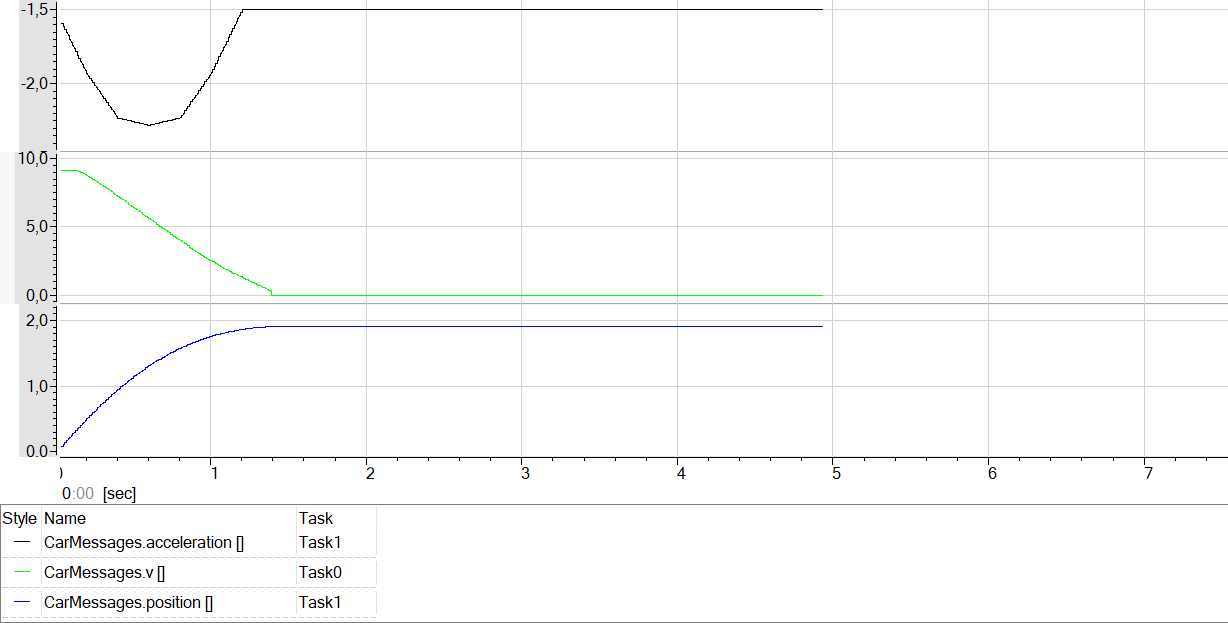
\includegraphics[width=1\textwidth]{images/ascet_acceleration.png}
\caption{ASCET car model}
\label{fig:D7_result}
\end{figure}

\chapter{D8: Implementation of pulse signal in ASCET}\label{cha:D8}

The pulse signal that has been implemented in Simulink (see chapter \ref{cha:D6}) is transferred to ASCET in this chapter.
The ASCET model consists of three sub-models described in three block diagrams. Two of the sub-models are regular classes that can be instantiated. This makes the whole model modular and the sub-models are able to be unit tested. One of the two classes calculates a frequency based on a given velocity and position of the car. The second class generates a pulse signal based on the calculated frequency.
The third class is a static class that passes the calculated frequency to the pulse signal generating class. The static class is also responsible for receiving the velocity and position messages of the car and pass them to the frequency computation class as well as sending the generated pulse signal as a new message. This can be seen in figure \ref{fig:BlockdiagrammFrequencyComputation} that shows the block diagram of the static class.

\begin{figure}[H]
\centering
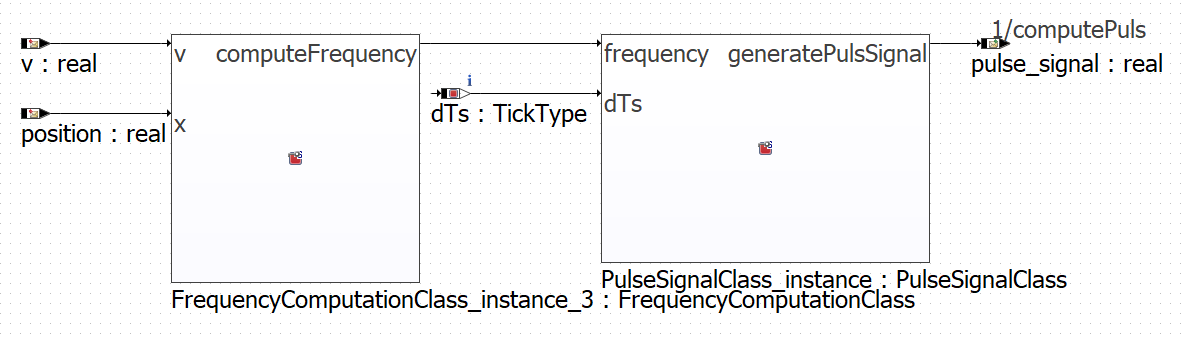
\includegraphics[width=1\textwidth]{images/Blockdiagramm_FrequencyComputation.png}
\caption{ASCET block diagram of static class $FrequencyComputation$}
\label{fig:BlockdiagrammFrequencyComputation}
\end{figure}

The frequency is calculated based on the Simulink implementation. However, in ASCET if-clauses with multiple conditions need to be implemented in series. The model can be seen in Figure \ref{fig:BlockdiagrammFrequencyComputationClass} and the sequencing process is described in the following:

\begin{enumerate}
\item If $x \geq 1.9m$, $v \leq 1.0$ and $v \textgreater 0.0$ return 10 (\textbf{1a} in Figure \ref{fig:BlockdiagrammFrequencyComputationClass})
\item Otherwise (\textbf{1b} in Figure \ref{fig:BlockdiagrammFrequencyComputationClass}) if $x \geq 1.0$, $v \leq 1.0$ and $v \textgreater 0.0$ find frequency in lookup table (\textbf{2a} in Figure \ref{fig:BlockdiagrammFrequencyComputationClass}). The lookup table is shown in Listing \ref{lst:D8_lookup}. If none of the conditions haven not been meet return 0 (\textbf{2b} in Figure \ref{fig:BlockdiagrammFrequencyComputationClass})
\end{enumerate}

\begin{lstlisting}[language=Java,basicstyle=\scriptsize, caption= ASCET frequency lookup table,label= lst:D8_lookup]
characteristic curve_cont frequency_lookup = {{1.0, 1.9}, {1.0, 9.0}};
\end{lstlisting}

\begin{figure}[H]
\centering
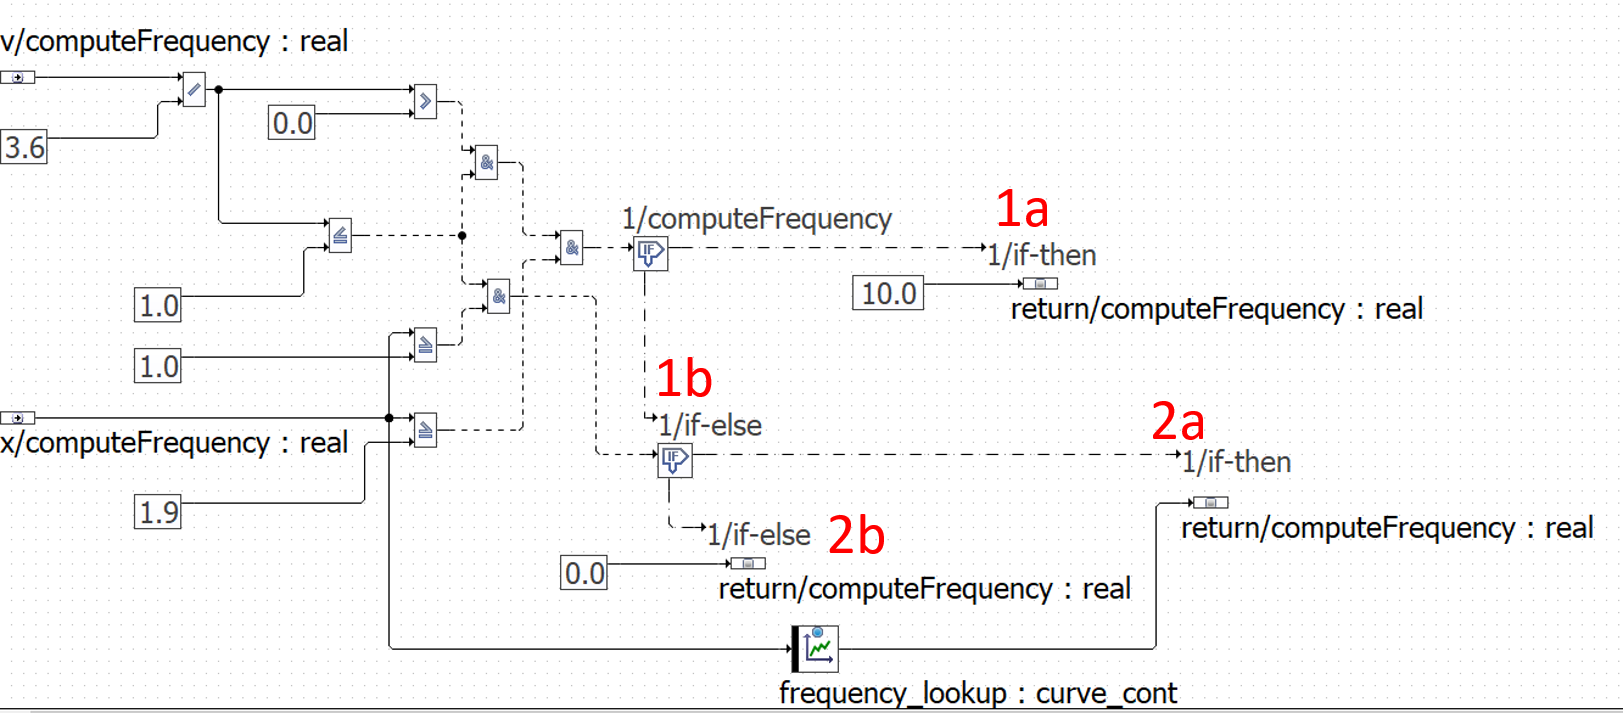
\includegraphics[width=1\textwidth]{images/Blockdiagramm_FrequencyComputationClassAnno.png}
\caption{ASCET block diagram of class $FrequencyComputationClass$}
\label{fig:BlockdiagrammFrequencyComputationClass}
\end{figure}

After the frequency has been calculated, it is passed to generate the pulse signal. If the frequency equals 10, the desired output is a continuous pulse. This means the pulse is set to 1 (\textbf{1a} in Figure \ref{fig:BlockdiagrammPulseSignal}). If however the frequency equals 0, no pulse is desired resulting in the pulse being set to 0 (\textbf{2a} in Figure \ref{fig:BlockdiagrammPulseSignal}). If $0 \textless frequency \textless 10$, the frequency is integrated to generate the pulse signal. For integration a time component is required. To be able to unit test the component, the time component is passed through a method argument. The frequency is integrated by multiplying frequency and time and adding the result to the previous results (\textbf{2b} in Figure \ref{fig:BlockdiagrammPulseSignal}). In Simulink it is possible to reset the integration block. Due to this not being possible in ASCET, the integrated frequency is reset as soon as the integrated frequency is greater or equal 1 because then one period is over and the new periodic time can be calculated (\textbf{2b} in Figure \ref{fig:BlockdiagrammPulseSignal}).  
While the integrated frequency is smaller or equal 0.5 the pulse signal is set to 1 (\textbf{3a} in Figure \ref{fig:BlockdiagrammPulseSignal}). Once the frequency is greater than 0.5 the pulse signal is set to 0 (\textbf{3b} in Figure \ref{fig:BlockdiagrammPulseSignal}). This means the signal is high for one half of a period and low for the other half of a period.

\begin{figure}[H]
\centering
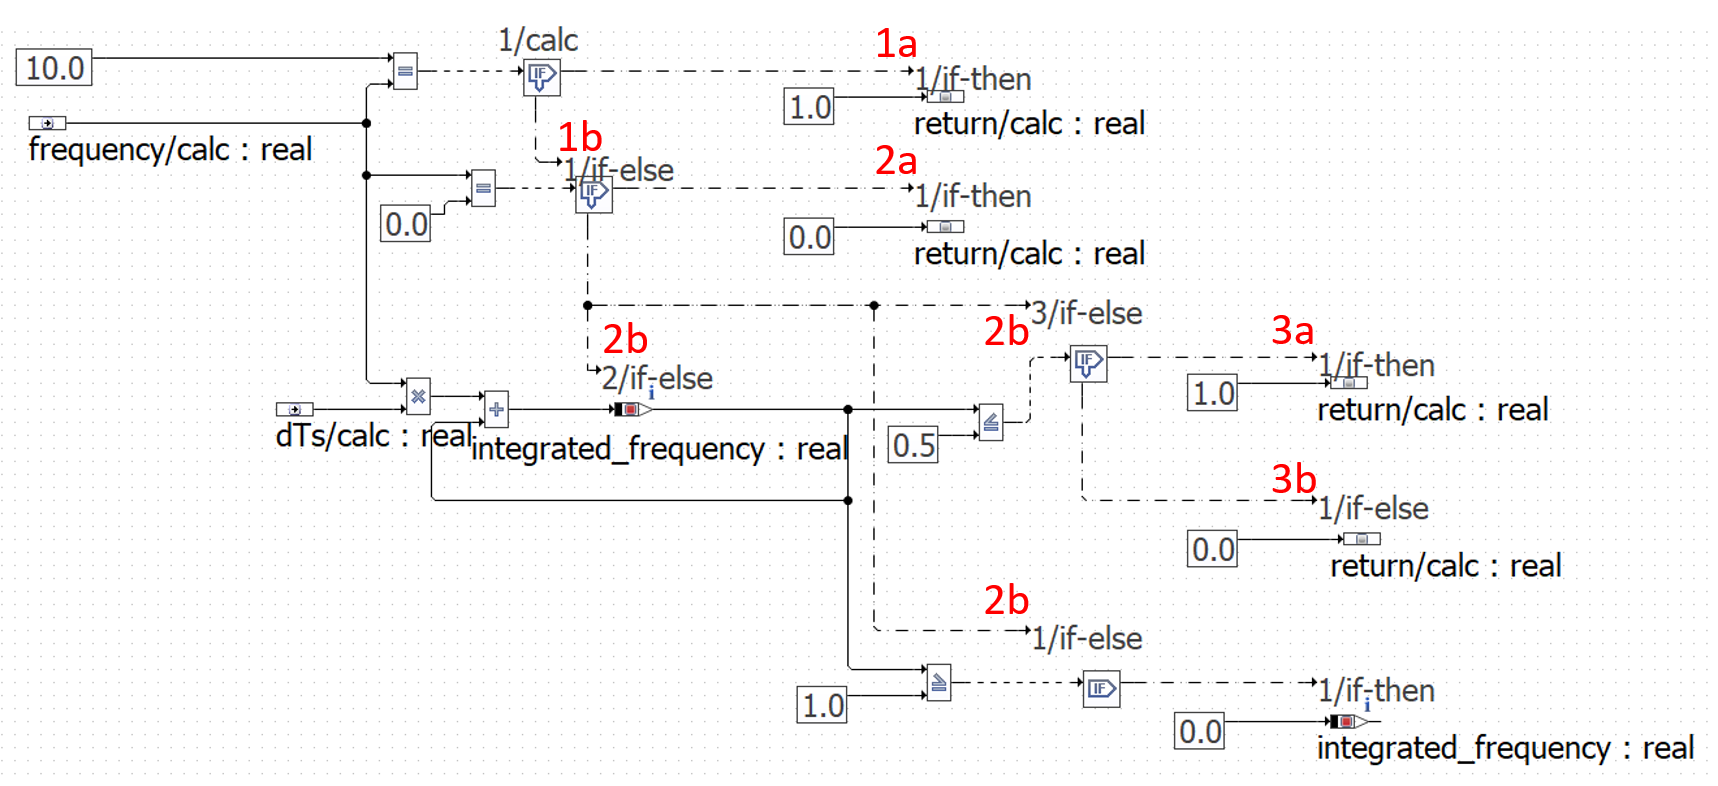
\includegraphics[width=1\textwidth]{images/Blockdiagramm_PulseSignalClassAnno.png}
\caption{ASCET block diagram of class $PulseSignalClass$}
\label{fig:BlockdiagrammPulseSignal}
\end{figure}

The resulting pulse signal is shown in Figure \ref{fig:BlockdiagrammPulseSignalOutput}. It shows that the period of the pulse signal is getting shorter once the car approaches the target position. The plot also shows that the pulse signal starts once the car is slower than 3.6 km/h (\^= 1m/s) and ends once the car is standing. The exact stopping position of the car is 1.905 m which is why the pulse signal becomes continuous for a short time and then gets reset, once the car stops. 

\begin{figure}[H]
\centering
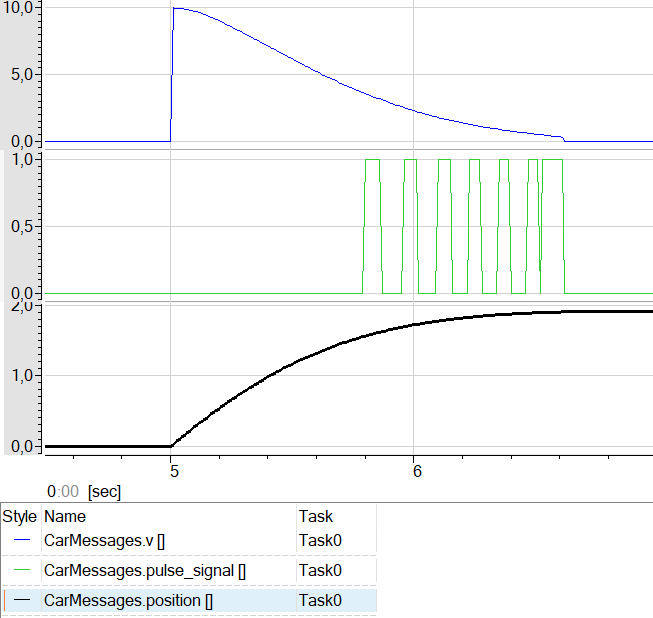
\includegraphics[width=1\textwidth]{images/ascet_pulsesignal.png}
\caption{Output pulse signal}
\label{fig:BlockdiagrammPulseSignalOutput}
\end{figure}

\chapter{D9: Implementation of unit tests for ASCET model parts}\label{cha:D9}
This section covers the unit tests of all components of the ASCET model.
The components are designed in a modular way to allow easy unit testing.
Also wrapper classes, passing messages into the components, are used to make it possible to unit test the components.
This is the only functionality the wrapper classes have.
That is necessary to make sure that no new bugs are introduced by the wrapper classes, because they can not be unit tested.\\
The unit tests are bundled in a package called $test$ in the ASCET project. The assertLib is imported for the assertions that are used in the unit tests. The unit tests are grouped by component with a static test class for each component. One test case corresponds to one method within the unit test classes.

Test cases are derived by analysing the requirements and finding equivalence classes.
The goal of the test case coverage is to cover every equivalence class and, in addition to that, select values that might result in errors based on experience.

\section{Unit tests for DriveModel}

$DriveModel$ computes acceleration, velocity, position and ultrasonic distance based on a defined time and brake pedal position. There are two equivalence classes. One equivalence class covers all velocities greater than 0.29 km/h and the other all velocities less or equal 0.29 km/h. As only one time step is simulated while unit testing the position will remain zero if the computed velocity is zero. Defined test cases can be seen in the table below.

\begin{table}[H]
\centering
\caption{Test cases for unit testing driveModel}
\begin{adjustbox}{width=1\textwidth, center=\textwidth}
\renewcommand{\arraystretch}{1}
\begin{tabular}{lllllll}
\textbf{Brake pedal} & \textbf{Time constant [s]} & \textbf{Acceleration [m/s]} &\textbf{Velocity [km/h]} & \textbf{Position [m]} & \textbf{Ultrasonic distance [m]} \\\hline
p = 0.0 & dTs = 1.0 & acc = -1.5 & v = 4.6 & s $\approx$ 1.278 & u $\approx$ 0.722\\
p = 0.5 & dTs = 0.1 & acc = -6.5 & v = 7.66 & s $\approx$ 0.213 & u $\approx$ 1.787\\
\label{tab:D10_drivemodel}
\end{tabular}
\end{adjustbox}
\end{table}

\section{Unit tests ParkAssistControllerTest}

$ParkAssistControllClass$ generates a brake pedal position based on a defined time using a look-up table.
There are two equivalence classes defined for the $ParkAssistControllClass$ that cover the brake pedal position if the time is inside the time span of the look-up table and if the time is greater than the time span of the look-up table.

\begin{table}[H]
\centering
\caption{Equivalence classes for unit testing ParkAssistControll}
\begin{adjustbox}{width=0.5\textwidth, center=\textwidth}
\renewcommand{\arraystretch}{1}
\begin{tabular}{lllllll}
\textbf{Time [s]} & \textbf{Output p(t)} \\\hline
$0 \leq t \leq 1.2$ &$ 0 \leq p(t) \leq 0.078$ \\
t > 1.2 & p(t) = 0\\
\end{tabular}
\end{adjustbox}
\end{table}

Based on the equivalence classes three test cases have been derived. Two test cases correspond to the first equivalence class and the third test case corresponds to the second equivalence class. 

\begin{table}[H]
\centering
\caption{Unit test test cases pulse signal frequency generation}
\begin{adjustbox}{width=0.5\textwidth, center=\textwidth}
\renewcommand{\arraystretch}{1}
\begin{tabular}{llll}
\textbf{Test case name} & \textbf{Time [s]} & \textbf{Expected brake pedal value} \\ \hline
time\textunderscore 0\textunderscore 0 & 0.0 & 0.0 \\
time\textunderscore 0\textunderscore 6 & 0.6 & 0.078 \\
time\textunderscore 2\textunderscore 0 & 2.0 & 0.0 \\                   
\end{tabular}
\end{adjustbox}
\label{tbl:D9_FrequencyGenerationTestCases}
\end{table}

\section{Unit tests FrequencyComputationTest}\label{sec:unitfrequency}

$FrequencyComputationClass$ generates a frequency based on a defined position and velocity using a look-up table.
There are three equivalence classes defined for the $FrequencyComputationClass$ class that cover three output scenarios: zero frequency, variable frequency based on a defined function (computed from look-up table) and continuous frequency. 

\begin{table}[H]
\centering
\caption{Equivalence classes for unit testing pulse signal frequency generation}
\begin{adjustbox}{width=1\textwidth, center=\textwidth}
\renewcommand{\arraystretch}{1}
\begin{tabular}{lllllll}
\textbf{Position} & \textbf{Velocity} & \textbf{Output} \\\hline
irrelevant & v = 0m/s or v > 1m/s & Zero\\
1 m <= s <= 1.9 m  & 0 m/s < v <= 1 m/s & $f(s)=-7.889\; Hz + 8.889*s\; Hz$\\
1.9 m < s <= 2 m  & 0 m/s < v <= 1 m/s & Continuous (10)
\end{tabular}
\end{adjustbox}
\end{table}

Table \ref{tbl:D9_FrequencyGenerationTestCases} shows the test cases derived from the equivalence classes above.
\begin{table}[H]
\centering
\caption{Unit test test cases pulse signal frequency generation}
\begin{adjustbox}{width=1\textwidth, center=\textwidth}
\renewcommand{\arraystretch}{1}
\begin{tabular}{llll}
\textbf{Test case name}               & \textbf{Velocity {[}m/s{]}} & \textbf{Position {[}m{]}} & \textbf{Expected frequency} \\ \hline
continuousPulse                       & 0.5                         & 1.91                      & 10                                    \\
noFrequencyBecauseVelocityHigh        & 1.5                         & 1                         & 1                                     \\
noFrequencyBecauseVelocityZero        & 0                           & 1.8                       & 0                                     \\
noFrequencyBecausPosition             & 0.9                         & 0.9                       & 0                                     \\
noFrequencyBecauseVelocityAndPosition & 1.1                         & 0.9                       & 0                                     \\
frequencyLow                          & 1.0                         & 1.0                       & 1                                     \\
frequencyHigh                         & 1.0                         & 1.9                       & 9                                     \\
frequencyMid                          & 1.0                         & 1.5                       & 5.44 < result \textless 5.45 
\end{tabular}
\end{adjustbox}
\label{tbl:D9_FrequencyGenerationTestCases}
\end{table}

\section{Unit tests PulseSignalClass}

$PulseSignalClass$ generates a pulse signal based on a defined frequency.
There are three equivalence classes defined for the $PulseSignalClass$ class that refer to the equivalence classes in section \ref{sec:unitfrequency}. 
The table below shows the equivalence classes for the pulse signal.
\begin{table}[H]
\centering
\caption{Equivalence classes for unit testing pulse signal}
\begin{adjustbox}{width=1\textwidth, center=\textwidth}
\renewcommand{\arraystretch}{1}
\begin{tabular}{lllllll}
\textbf{Position} & \textbf{Velocity} & \textbf{Pulse Signal} \\\hline
irrelevant & V = 0m/s oder V > 1m/s & Zero\\
1m <= X <= 1.9m  & 0m/s < V <= 1m/s & Alternating 0,1\\
1.9m < X <= 2m  & 0m/s < V <= 1m/s &Continuous
\end{tabular}
\end{adjustbox}
\end{table}

The derived test cases are shown below.

\begin{table}[H]
\centering
\caption{Pulse signal test cases}
\renewcommand{\arraystretch}{1}
\begin{tabular}{lll}
\textbf{Frequency} & \textbf{dts} & \textbf{Expected result} \\\hline
0         & 1   & 0               \\
1         & 0.1   & 1               \\
1         & 0.6   & 0               \\
10        & 1   & 1              
\end{tabular}
\end{table}

\chapter{D10: Development and implementation of a system test environment for ASCET simulation}\label{cha:D10}

The system test environment in Figure \ref{fig:D10} features an oscilloscope and several textboxes. 
The oscilloscope shows the velocity, acceleration and position of the car as well as the ultrasonic distance signal and the pulse signal. The textboxes show the value of the signal in the oscilloscope next to them. 
The checkbox at the right bottom shows whether the car did a full brake within less than 2m.

With the parameters that have been evaluated in this project, the car stops at 1.905 m.

\begin{figure}[H]
\centering
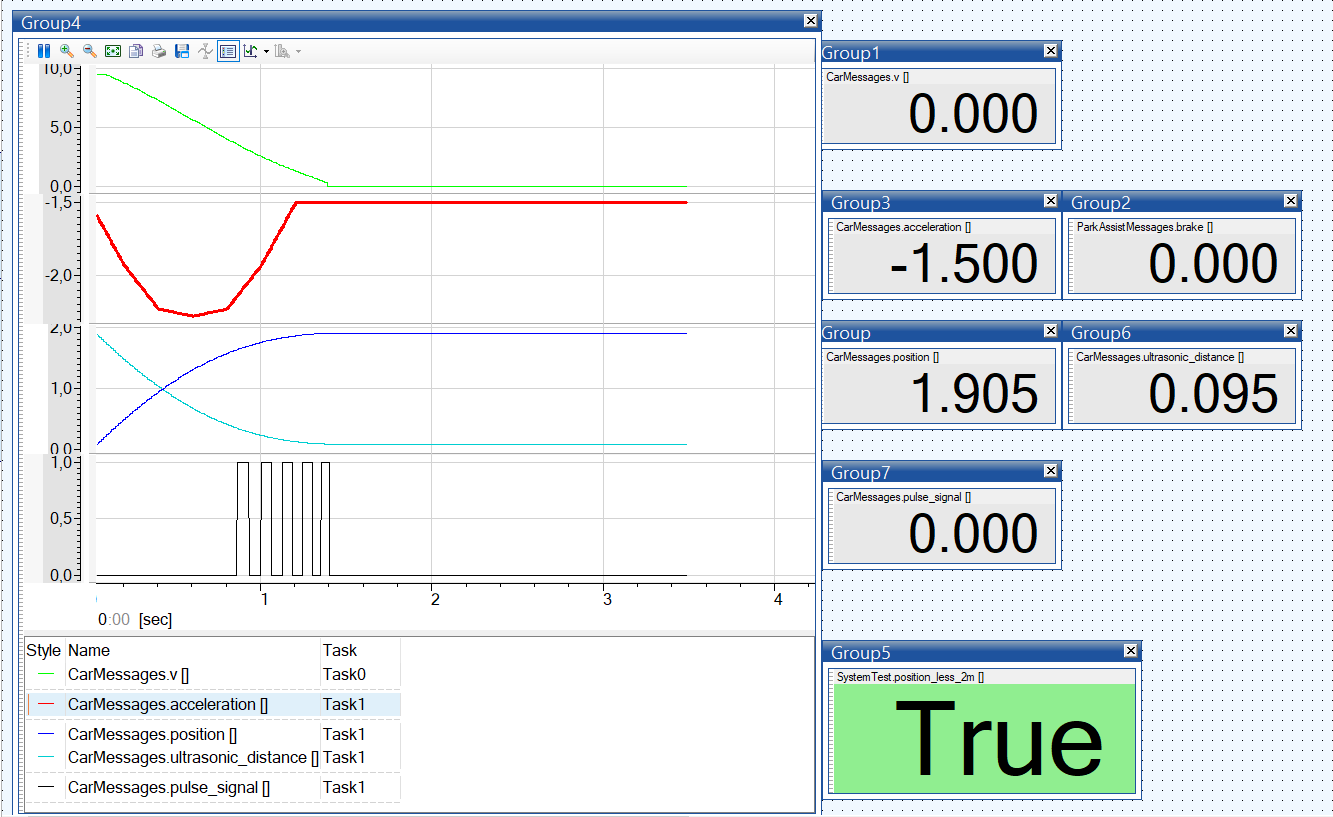
\includegraphics[width=1\textwidth]{images/ascet_experiment_environment.png}
\caption{ASCET Experiment Environment}
\label{fig:D10}
\end{figure}

For monitoring whether the car stopped within 2 m, a new class is introduced that is shown in Figure \ref{fig:D10_systest}. As can be seen in the block diagram, the class consists of a simple check whether the velocity is zero and the position less than 2 m. 

\begin{figure}[H]
\centering
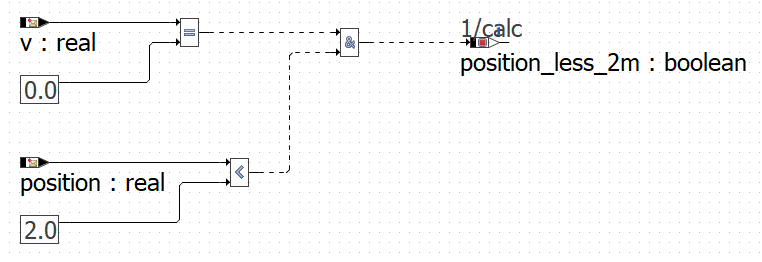
\includegraphics[width=1\textwidth]{images/Blockdiagramm_systemtest.png}
\caption{ASCET block diagram of $SystemTestEnvironment$}
\label{fig:D10_systest}
\end{figure}


\chapter{D11*: Plausibility check comparing measured velocities and distances}\label{cha:D11}
The distance signal from the ultrasonic sensor (in case there is a non-moving object in front of it) and the measured car velocity are two measurements that provide independent measurement of travelled distance.\\
In the given scenario it is known that a non-moving object is 2 m in front of the car. So the ultrasonic sensor can be used to compute travelled distance by comparing consequent distance measurements. E. g. if the distance measurement before was 0.8 m to the object ahead and the next measurement was 0.6 m, the car travelled a distance of 20 cm.\\
Integrating the velocity also provides a measurement of the travelled distance. These two measurements provide a redundancy in measuring travelled distance. If these measurements would be significantly different, one of the measurements must be inaccurate.\\
If the object in front of the ultrasonic sensor is moving or if there is no object at all, this procedure can not be used.\\
\chapter{D13*: Impact of inaccuracies}\label{cha:D13}
\section{Ultrasonic Sensor}
Using one ultrasonic sensor has limits when measuring distance to objects while parking.
Several scenarios can be imagined, in which a distance measurement from one ultrasonic sensor does not provide enough information to securely park without causing an accident.
The scenario in \ref{fig:D13_USLimitAbove} shows the limits of one ultrasound sensor. One ultrasonic sensor in the middle of the front of the car might not be able to detect the two poles. In this case parking based on the information of the ultrasonic sensor might result in an accident.
Using multiple ultrasonic distributed over the front of the vehicle might be able to resolve such an issue.
\begin{figure}[H]
\centering
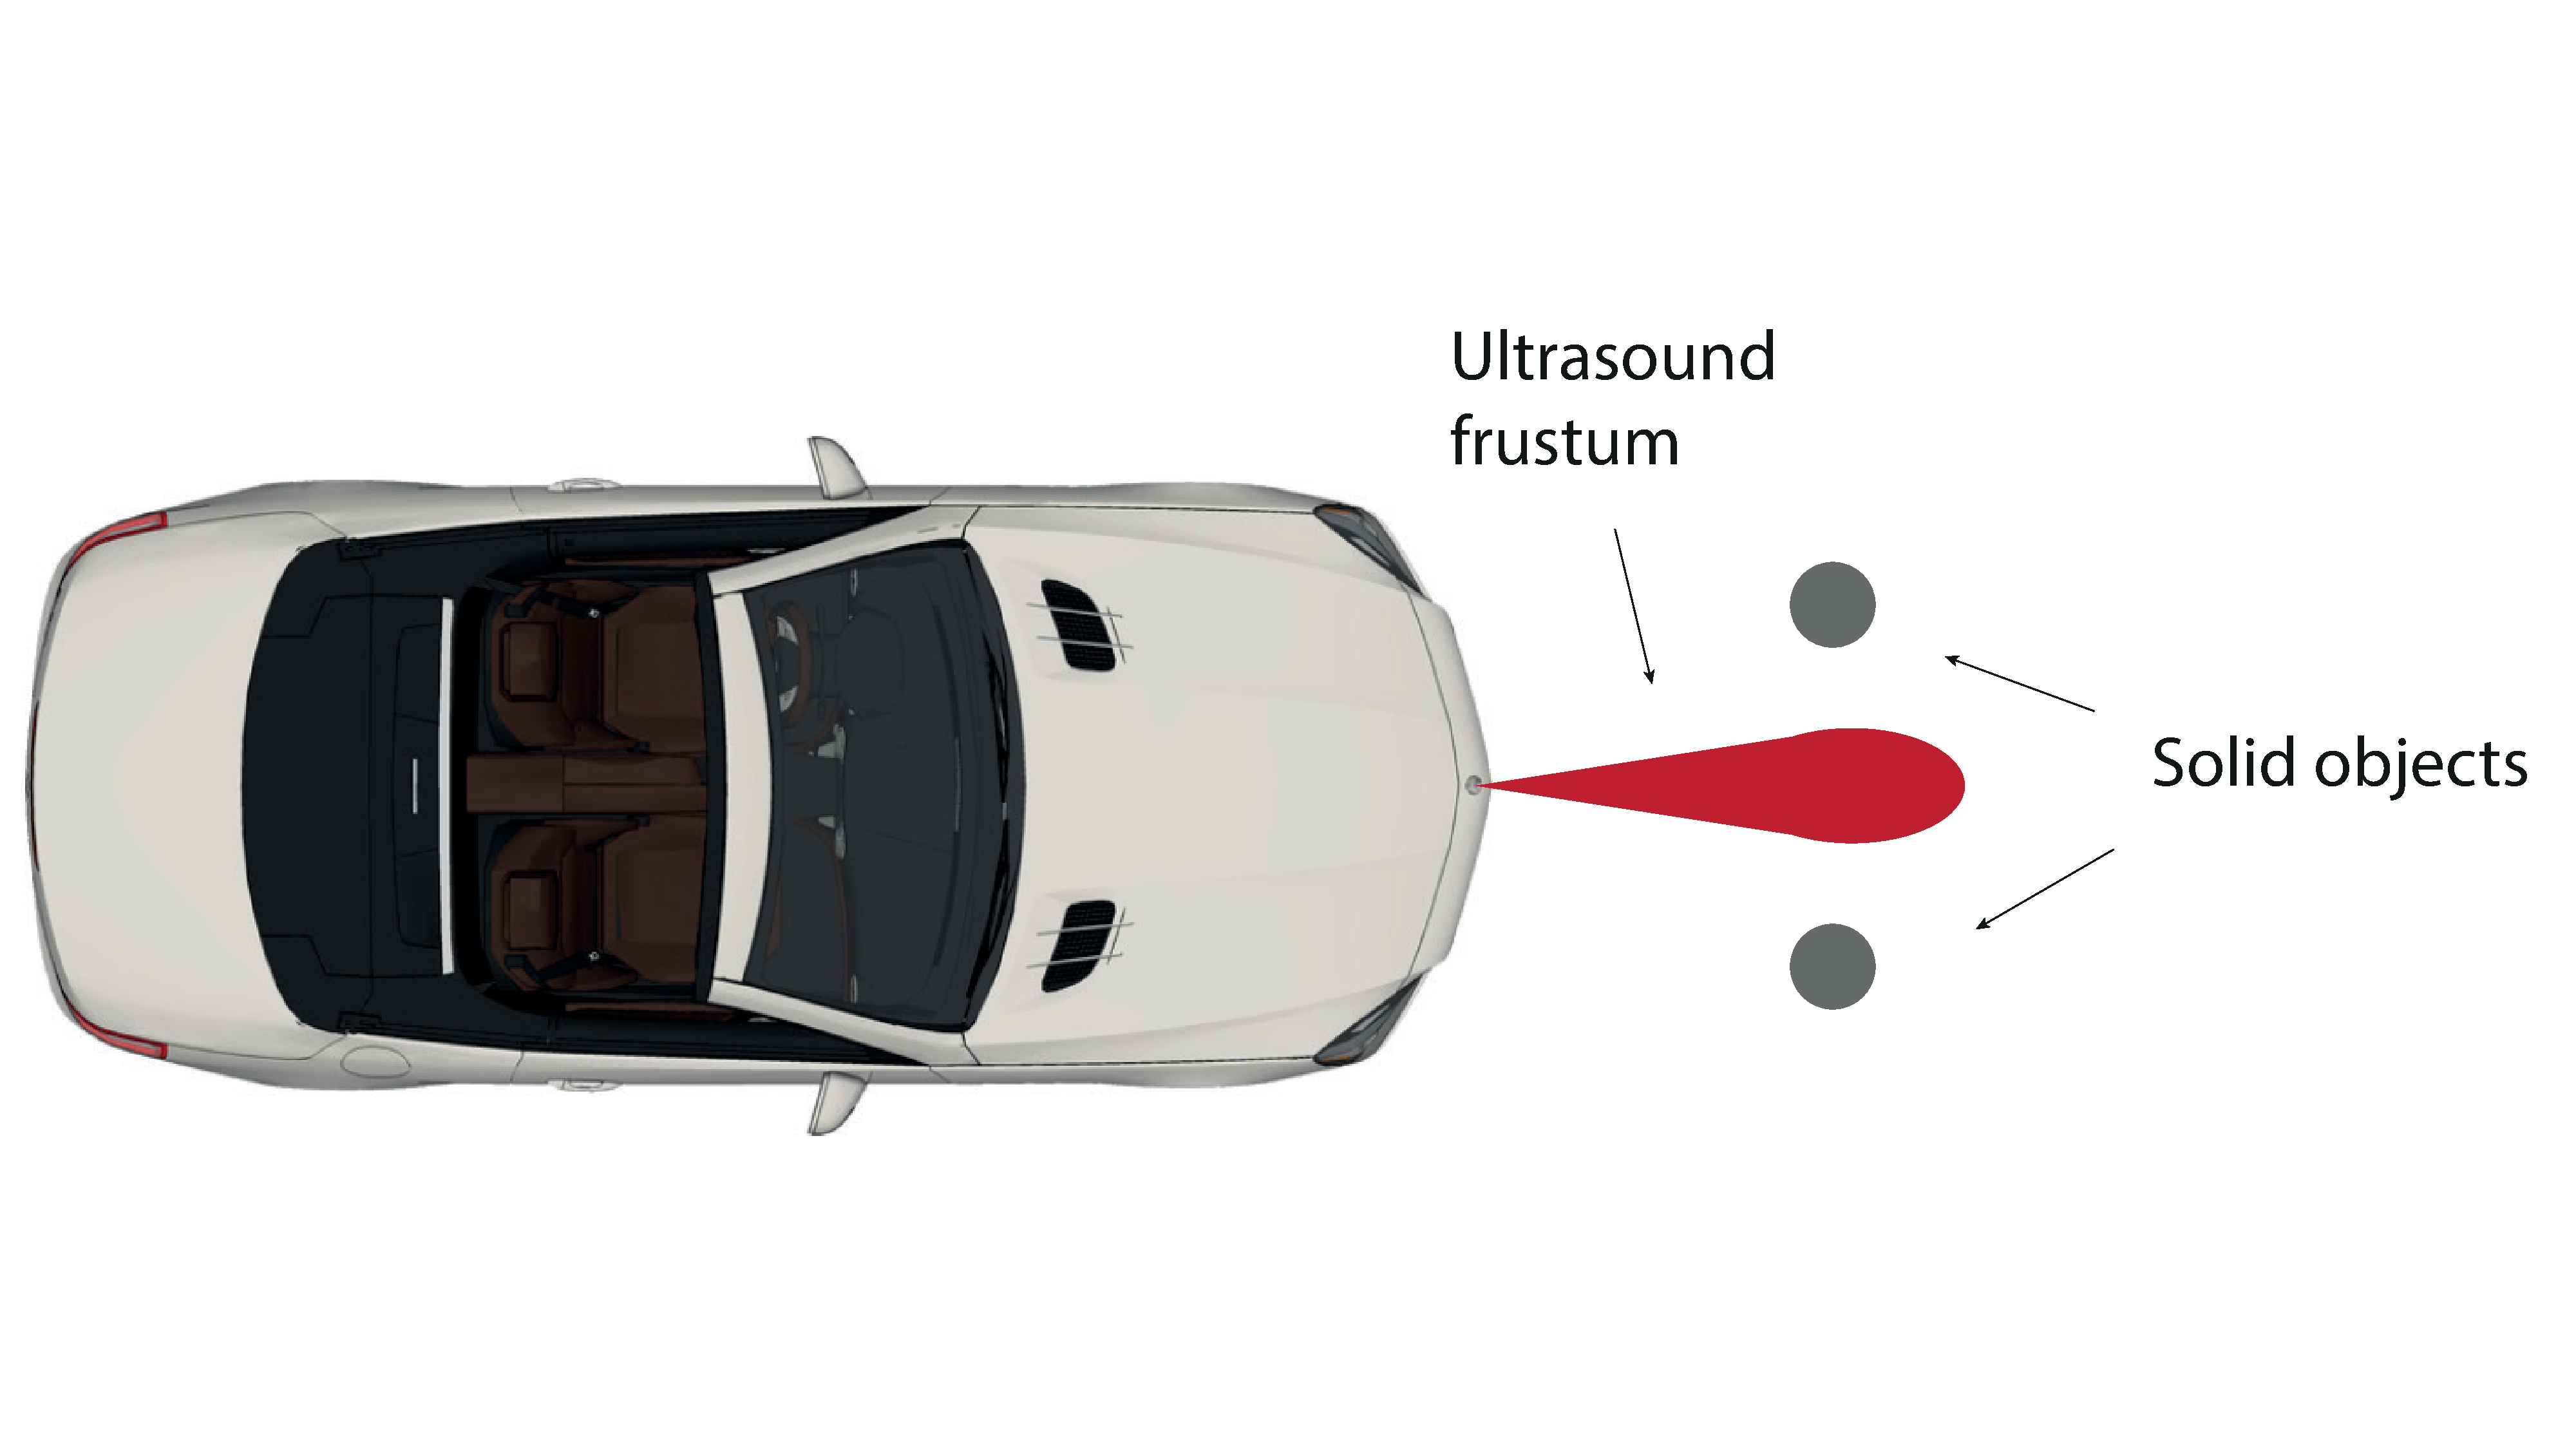
\includegraphics[width=.7\textwidth]{images/us_drawing.pdf}
\caption{Ultrasonic sensor limits}
\label{fig:D13_USLimitAbove}
\end{figure}
With one ultrasonic sensor, also blind spots over and under an ultrasonic sensor can occur.
Figure \ref{fig:D13_USLimitSide} demonstrates that.
Depending on the used sensor, the sensor frustum might vary, but the concept remains the same.
If there is an object above the sensor frustum (for example a gate) it might not be detected by the ultrasonic sensor.
Then the driver would have to intervene, because he would probably see the object.
But then the driver would be responsible for safe parking, not the ParkAssist.


\begin{figure}[H]
\centering
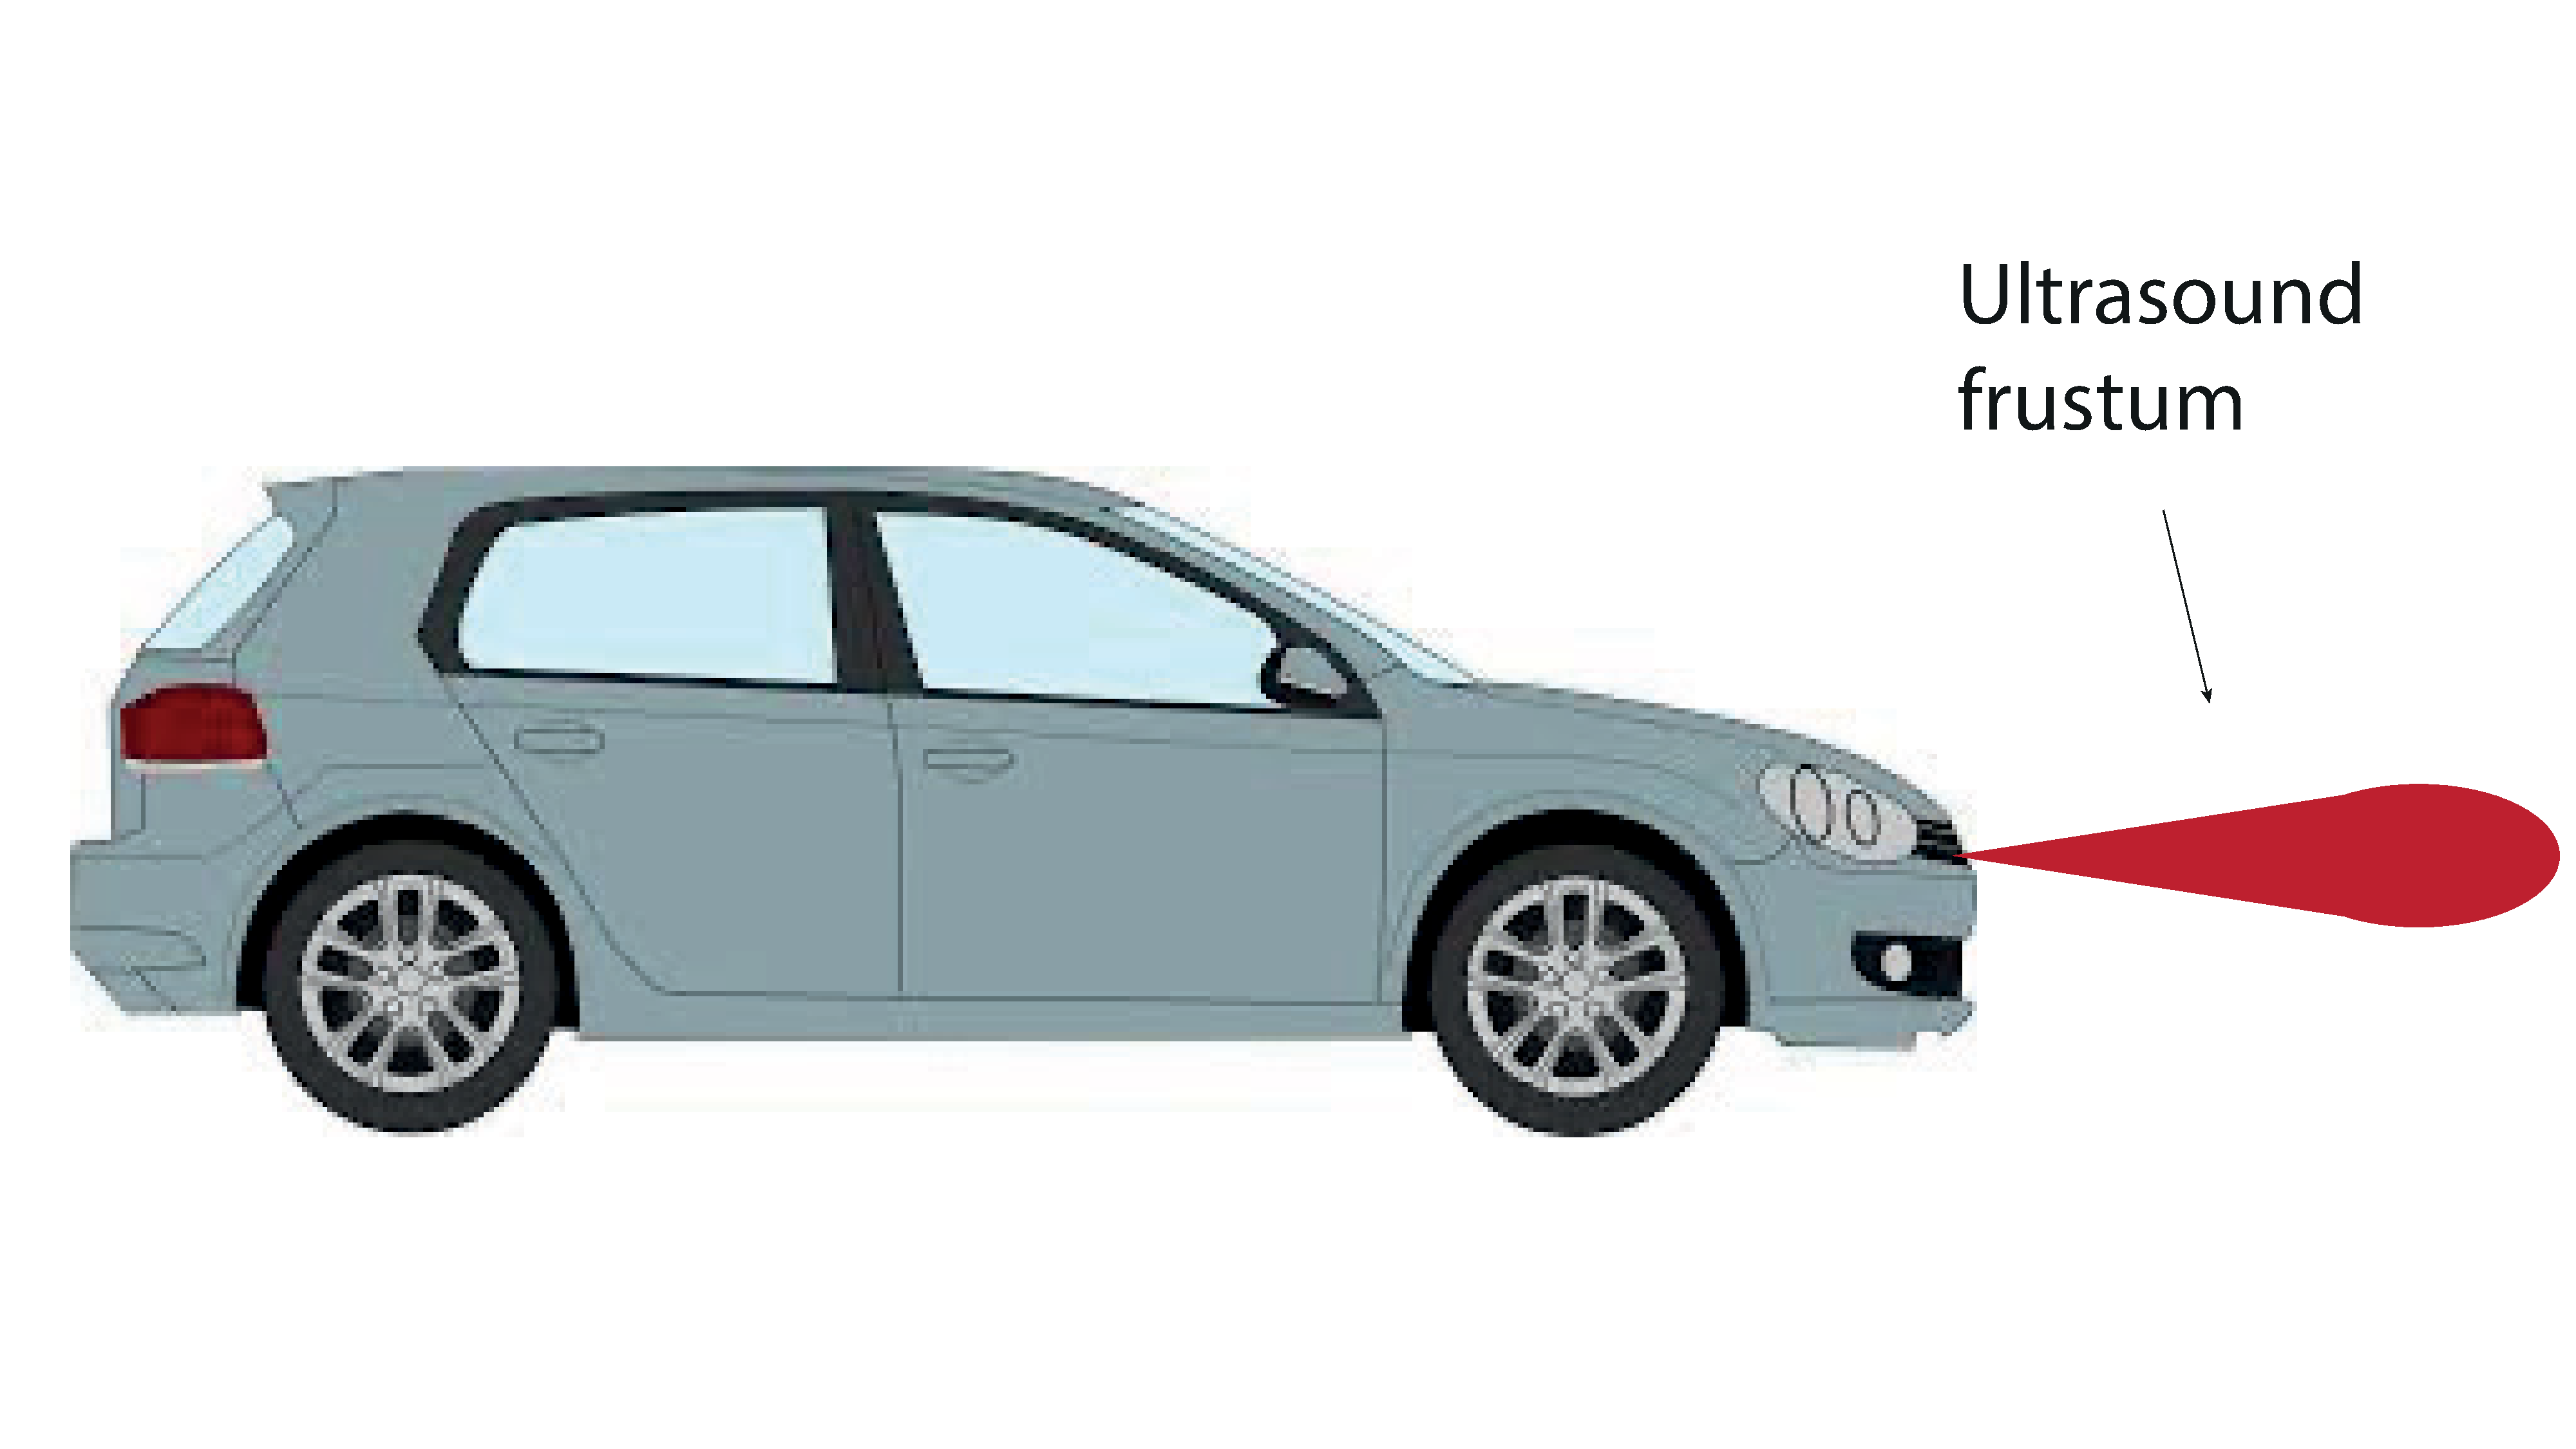
\includegraphics[width=.7\textwidth]{images/us_drawing2.pdf}
\caption{Ultrasonic sensor limits}
\label{fig:D13_USLimitSide}
\end{figure}

The inaccuracy of the ultrasonic sensor of +/- 2 cm does not have an influence on the current p(t).
But if a feedback controller would be used, that relies on the distance information to brake, the inaccuracy would have an influence on the braking procedure.
The inaccuracy would have to be considered. Using multiple sensors might be a way to reduce the inaccuracy. Also using a safety margin when parking is reasonable.


zeit inaccuracies
\section{Velocity measurement sensor}
-see chapter \ref{cha:D5}

\chapter{D14*: Reflection}\label{cha:D14}
-only 2 meter stop considered
-ultrasonic reichweite
-no feedback

-no air friction, but relatively low at low speed
-1.5 friction
-sensor inaccuracies normally follow a statistic distribution and do not have discrete borders

-parkassist limits

\section{Model inaccuracies}
-model not realistic
\section{Computation inaccuracies}
-rundungsfehler